\documentclass[a4paper,11pt]{report}
%\documentclass[a4paper,12pt]{article}
\usepackage[backend=biber,sorting=ydnt,maxnames=18,giveninits=true,labelnumber=true,defernumbers=true]{biblatex}
%\usepackage[backend=biber,sorting=ydnt,maxnames=18,giveninits=true,labelnumber=true,defernumbers=true]{biblatex}
%\usepackage[backend=biber,sorting=ydnt,maxnames=18,giveninits=true]{biblatex}
%\usepackage[bibstyle=publist]{biblatex}
\usepackage{xstring}
\usepackage{url}
\usepackage{booktabs}
\usepackage{hyperref}
\usepackage{color}

%\usepackage[tocflat]{tocstyle}
\usepackage[tocgraduated]{tocstyle}
%\usetocstyle{standard}
%\usetocstyle{KOMAlike}
\usetocstyle{classic}
%\usetocstyle{allwithdot}

\renewcommand*\contentsname{Table of Contents}

\usepackage{enumitem}
\newlist{yearlist}{description}{10}
\setlist[yearlist]{itemindent=0pt,labelwidth=2cm,leftmargin=2cm,listparindent=0pt,labelsep=0pt,font=\normalfont}%,itemsep=3pt}

%\newlist{commentlist}{itemize}{10}
%\setlist[commentlist]{itemindent=0pt,labelwidth=0.5cm,leftmargin=0.5cm,listparindent=0pt,labelsep=0pt,font=\normalfont}
%\setlist[commentlist]{itemindent=0pt,labelwidth=2cm,leftmargin=2cm,listparindent=0pt,labelsep=0pt,font=\normalfont}

\usepackage{titlesec}
\definecolor{gray75}{gray}{0.75}
\newcommand{\hsp}{\hspace{20pt}}
\titleformat{\chapter}[hang]{\huge\bfseries}{\thechapter\hsp\textcolor{gray75}{|}\hsp}{0pt}{\huge\bfseries}
\titlespacing*{\section}{0pt}{6pt plus 1pt minus 0.5pt}{3pt plus 0.5pt}
\titlespacing*{\chapter}{0pt}{12pt plus 1pt minus 0.5pt}{6pt plus 0.5pt}
\titlespacing*{\subsection}{0pt}{6pt plus 1pt minus 0.5pt}{3pt plus 0.5pt}
%\titlespacing*{\subsection}{0pt}{5.5ex plus 1ex minus .2ex}{4.3ex plus .2ex}

\titlespacing*{\paragraph}
{0pt}{3pt plus 1pt minus 0.5pt}{3pt plus 2pt minus 0.5pt}

\usepackage{enumitem}
\setlist{nosep}

\usepackage{tcolorbox}

\usepackage{fontspec}
\setmainfont{Cambria}
\setsansfont{Calibri}

%\setlength{\itemsep}{0pt plus 1pt}
%\setlength{\itemsep}{0pt}
%\setlength{\topsep}{0pt}
\setlength{\parskip}{3pt plus 0.5pt minus 0.5pt}
%\setlength{\beforeskip}{3pt}


\usepackage[scale=0.85]{geometry}

\geometry{
 a4paper,
 total={170mm,257mm},
 left=20mm,
 top=20mm,
 }

%\assignrefcontextkeyws[labelprefix=C]{C}
%\assignrefcontextkeyws[labelprefix=J]{J}

\addbibresource{bib/varrodan.bib}
\addbibresource{bib/external.bib}
%\addbibresource{bib/pcmember.bib}
%\addglobalbib{bib/external.bib}

%\assignrefcontextkeyws[labelprefix=C]{C}
%\assignrefcontextkeyws[labelprefix=J]{J}

\defbibheading{subbibliography}[\refname]{\subsection{#1}}
\defbibheading{subbibintoc}[\refname]{\subsection{#1}}
%\defbibheading{subbibliography}[\refname]{\subsection*{#1}}
%\defbibheading{subbibintoc}[\refname]{\subsection*{#1}}

\renewcommand*{\mkbibnamegiven}[1]{%
%\ifpartannotation{family}{self}{\textbf{#1}}{#1}}
\ifpartannotation{family}{self}{\ifcategory{mcgill}{\mkbibbold{\underline{#1}}}{\textbf{#1}}}{#1}}

\renewcommand*{\mkbibnamefamily}[1]{%
\ifpartannotation{family}{student}{#1\textsuperscript{*}}{%
%\ifpartannotation{family}{self}{\textbf{#1}}{#1}}}
\ifpartannotation{family}{self}{\ifcategory{mcgill}{\mkbibbold{\underline{#1}}}{\textbf{#1}}}{#1}}}

\renewcommand*{\bibfont}{\small}

\usepackage{fancyhdr}
\pagestyle{fancy}\lhead{Dossier in Support of Application for Tenure} \rhead{August 2019}
\rhead{Dániel Varró} \lfoot{} \rfoot{\bf \thepage} \cfoot{}

%\title{Teaching Portfolio}
%\author{D\'aniel Varr\'o}
%\date{August 2019}

\DeclareRefcontext{bref}{labelprefix=B}
\DeclareRefcontext{jref}{labelprefix=J}
\DeclareRefcontext{cref}{labelprefix=C}
\DeclareRefcontext{wref}{labelprefix=W}
\DeclareRefcontext{oref}{labelprefix=O}
\DeclareRefcontext{eref}{labelprefix=E}
\DeclareRefcontext{iref}{labelprefix=I}
\DeclareRefcontext{pcref}{labelprefix=PC}
\DeclareRefcontext{chref}{labelprefix=CH}
\DeclareRefcontext{scref}{labelprefix=SC}
\DeclareRefcontext{loref}{labelprefix=LO}
\DeclareRefcontext{dsref}{labelprefix=DS}
\DeclareRefcontext{jrref}{labelprefix=JR}
\DeclareRefcontext{ijref}{labelprefix=IJ}
%\DeclareRefcontext{extref}{labelprefix=X,sorting=none}
\DeclareRefcontext{extref}{sorting=none}
\DeclareBibliographyCategory{own}
\DeclareBibliographyCategory{mcgill}

\begin{document}

\begin{titlepage}
\thispagestyle{empty}
\newcommand{\HRule}{\rule{\linewidth}{0.5mm}} % Defines a new command for the horizontal lines, change thickness here

\center % Center everything on the page
 
%----------------------------------------------------------------------------------------
%	HEADING SECTIONS
%----------------------------------------------------------------------------------------

\includegraphics[width=.5\textwidth]{figures/McGill-logo.png}\\[0.5cm] 

\textsc{\LARGE Department of Electrical and Computer Engineering}\\[3cm] 
%\textsc{\Large Major Heading}\\[0.5cm] % Major heading such as course name
%\textsc{\large Minor Heading}\\[0.5cm] % Minor heading such as course title

\HRule \\[0.4cm]
{ \huge \bfseries Dossier in Support of Application for Tenure}\\[0.4cm] % Title of your document
\HRule \\[4cm]

%\large \emph{by}\\
{\bfseries\LARGE Dániel \textsc{Varró}}\\[8cm] % Your name

%\flushleft
%\large
%Department of Electrical and Computer Engineering \\
%3480 Rue University, Montréal, Québec, \\ 
%H3A 0E9, Canada 
%\center 

{\Large September 2019}\\[2cm] 

\vfill % Fill the rest of the page with whitespace
\end{titlepage}

\thispagestyle{empty}
~
\newpage

\setcounter{page}{1}
{%\footnotesize
\small
\tableofcontents
}

\chapter{Curriculum Vitae}
\label{sec:curriculum-vitae}
\lfoot{Curriculum Vitae} 
%\rfoot{Curriculum Vitae} 

\section{Personal Details}

\begin{tabular}{@{}lp{12cm}@{}}
\toprule
%\textbf{ECSE 429 Questions} & \textbf{F18} \\ 
%\toprule
%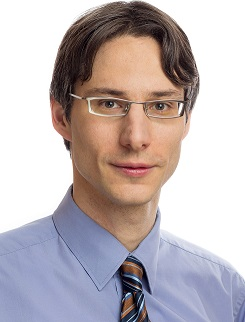
\includegraphics[width=.2\textwidth]{figures/VarroD-2015-small.jpg} &  \\ \midrule
Full name:  & Dániel Varró \\ %\midrule
Contact address: &  %McConnell Engineering Building \newline
Department of Electrical and Computer Engineering \newline
McGill University \newline
3480 Rue University, Montreal, QC, Canada, H3A 0E9\\ %\midrule
Phone: &  +1-514-3983681 \\ %\midrule
Email: &  \href{mailto:daniel.varro@mcgill.ca}{daniel.varro@mcgill.ca} \\ %\midrule
\bottomrule
\end{tabular}

\section{Education and Degrees}

\begin{yearlist}
\item[2013] Doctor of Science (DSc); Hungarian Academy of Sciences  
\item[2011] Habilitation; Budapest University of Technology and Economics (in short: BME) 
\item[2004] PhD in Software Engineering (official name: Technical Informatics); BME
\item[2000] MSc in Software Engineering (official name: Technical Informatics); BME 
\end{yearlist}

%\newline This degree is a formal prerequisite of full professorship in Hungary. \\


\section{Academic and Professional Experience}
\subsection{Academic positions}
\begin{yearlist}
\item[2016-] Professor, Electrical and Computer Engineering (ECE) Department, McGill University
\item[2015- 2020] Research Chair of MTA-BME Lendület Cyber-Physical Systems Research Group; \\ Hungarian Academy of Sciences 
\item[2014-] Professor, Dept. of Measurement and Inf. Systems, BME  (on unpaid leave since 08/2016)
\item[2014] Visiting Professor, Dept. of Computer Science, McGill University, Canada
\item[2014] Visiting Professor, D\'epartemente d'informatique et de recherche op\'ertionnelle (DIRO), Universit\'e de Montr\'eal, Canada
\item[2009-2014] Associate Professor (tenured), Dept. of Measurement and Inf. Systems, BME 	
\item[2005-2009] Assistant Professor, Dept. of Measurement and Information Systems, BME 
\item[2003-2005] Lecturer, Dept. of Measurement and Information Systems, BME
\end{yearlist}

\subsection{Research visits} 
\begin{yearlist}
\item[2014] Universit\'e de Montr\'eal (Prof. Houari Sahraoui) and McGill University (Prof. Hans Vangheluwe),  6 months
\item[2005] TU Berlin, Germany (1 month, with Prof. Hartmut Ehrig, SEGRAVIS Grant)
\item[2004] TU Berlin, Germany (1 month, with Prof. Hartmut Ehrig, SEGRAVIS Grant)
\item[2003] Univ. Paderborn, Germany (3 months, with Prof. Gregor Engels, SEGRAVIS) 
\item[2001] SRI International, US (4 months, with Dr. John Rushby) 
\end{yearlist}

\subsection{Industrial positions and entrepreneurship} 
\begin{yearlist}
\item[2013-] Co-founder of IncQuery Labs Ltd. (Co-founder and Strategic advisor) 
\item[2006-2014] Co-founder and Vice-President of Research and Development at OptXware Ltd. 
\end{yearlist}

\subsection{Membership in professional societies and committees}
\begin{yearlist}
\item[2018-] \textbf{Member}: The McGill Sustainability Systems Initiative (MSSI)
\item[2016-] \textbf{Member}: McGill Institute for Aerospace Engineering (MIAE)
\item[2011-] 3x \textbf{Elected member}: Informatics Committee of Hungarian Academy of Sciences (a total of 15 senior members are elected in the field of in computer science and software engineering)
\item[2009-2015] \textbf{Vice president}: John von Neumann Computer Society 
\item[2006-] \textbf{Member}: IEEE Computer Society 
\end{yearlist}


\section{Awards and Honors} 

Six major awards since affiliated to McGill University. 
\begin{yearlist}
\item[2018] \textbf{Distinguished Reviewer Award} (at ICSE 2018: 40th (IEEE/ACM) International Conference on Software Engineering: 11 out of 101 program committee members)
\item[2018] \textbf{Best Tool Paper Award} (at MODELS 2018: ACM/IEEE 21st Int. Conference on Model Driven Engineering Languages and Systems: 1 out of 10 tool papers)
\item[2018] \textbf{EASST Best Paper Award} (at ETAPS 2018: European Joint Conferences on Theory and Practice of Software: selected 1 out of over 140 papers)
\item[2017] \textbf{Csanád Imreh Award} (by OTDT Hungary): \newline I was the first ever awardee of the prize (awarded in the field of software engineering and computer science for Hungarian researchers below the age of 41) commemorating the Hungarian computer scientist who tragically died in 2017 at the age of 41.  
\item[2016] ACM \textbf{Distinguished Paper Award} (at MODELS 2016: 19th IEEE/ACM International Conference on Model Driven Engineering Languages and Systems) 
\item[2016] IEEE \textbf{10-Year Most Influential Paper Award} \newline (at VL/HCC 2016: IEEE Symposium on Visual Languages \& Human-Centric Computing for a paper presented at VL/HCC 2005 conference) 
\newline
\rule{\linewidth}{0.2mm}
%\hrule
\item[2014] Springer \textbf{10-Year Most Influential Paper Award} \newline (at MODELS 2014: 17th IEEE/ACM International Conference on Model Driven Engineering Languages and Systems for a paper presented at UML2004 conference) 
\item[2014] \textbf{Best Paper Award} (at IEEE CSMR-WCRE 2014 Software Evolution Week) 
\item[2014] \textbf{STEM Award} by Tempus Foundation for innovative education methods (introducing Apache VCL cloud-based labs)
\item[2013] Springer \textbf{Best Paper Award} (MODELS 2013: 16th IEEE/ACM International Conference on Model Driven Engineering Languages and Systems: 1 out of 47 accepted papers) 
\item[2011] ACM \textbf{Distinguished Paper Award} (ASE 2011: 26th IEEE/ACM International Conference on Automated Software Engineering) 
\item[2010-2013] \textbf{J\'anos Bolyai Scholarship} (Design and Analysis Techniques for the Certification of Model Transformations): A national award of the Hungarian Academy of Sciences for young scholars. It can be awarded
at most twice in lifetime.
\item[2009] \textbf{Distinguished Tutor}: Bi-annual award for the supervision of MSc students carrying out early research with 3 awardees in Computer Science biannually. It requires 10 years of successful tutoring (I became the youngest ever awardee). 
\item[2009] Springer \textbf{Best Paper Award} and ACM \textbf{Distinguished Paper Award} (MODELS
2009: The 12th IEEE/ACM International Conference on Model Driven Engineering Languages and Systems: 1 out of 58 papers) 
\item[2005-2008] \textbf{J\'anos Bolyai Scholarship} (Design and Analysis Techniques for Automated Model Transformations) 
\item[2003] \textbf{J\'anos Kem\'eny Prize } (An annual award in Hungary for young scholars below the age of 35 issued by the John von Neumann Computer Society)
\end{yearlist}

\section{Invited Talks}

A career total of 37 invited talks, 8 invited talks since joining McGill University. 

\begin{yearlist}
\item[2018] Design space exploration for graph model generation  (Search Based Model Engineering Workshop at King's College London) 
\item[2017] \textbf{Keynote talk}: Automated Graph Model Generation for Smart and Safe Cyber-Physical Systems (Consortium for Software Engineering Research CSER 2017)
\item[2017] Incremental Queries and Reactive Transformations (DSM-TP 2017 Int. Summer School)
\item[2017] Formal Verification and Validation in Domain-Specific Languages (DSM-TP 2017 Summer School)
\item[2016] Graph-based  Design and Analysis Tools for Smart and Safe Cyber-Physical Systems (NASA Jet Propulsion Lab) 
\item[2016] Model-based Tools for Engineering Cyber-Physical Systems (McGill University Professor Talks)
\item[2016] Scalable  Graph-based techniques for smart cyber-physical systems (Papyrus Industrial Consortium)
\item[2016] Incremental Model Queries and Transformations (DSM-TP 2016 International Summer School) 
\newline
\rule{\linewidth}{0.2mm}
\item[2016] Models and Queries for Smart and Safe Cyber-Physical Systems (CSCS 2016 Conference, Szeged)
\item[2016] Challenges for Smart and Trustworthy Cyber-Physical Systems (Ericsson University Day 2016 Budapest)
\item[2016] \textbf{Keynote talk}: Incremental Queries and Transformations: From Concepts to Industrial Applications  (SOFSEM 2016: 42nd Int. Conf. on Current Trends in Theory and Practice of Computer Science) 
\item[2015] EMF/Ecore-based DSL engineering (at Dagstuhl \#15062:  Domain-Specific Languages)
\item[2015] EMF-IncQuery: Incremental Evaluation of Model Queries (DSM-TP 2015 Int. Summer School)  
\item[2015] VIATRA: Advanced Tools by Reactive Transformations (DSM-TP 2015 Int. Summer School) 
\item[2014] \textbf{Plenary Talk}: Generic and Meta-Transformations (Most Influential Paper Presentation at @MODELS 2014, Valencia, Spain)
\item[2014] Incremental Model Queries over the Cloud (SERENE 2014 Int. Autumn School, Hungary)
\item[2014] EMF-IncQuery: Incremental Evaluation of Model Queries (DSM-TP 2014 Int. Summer School)
\item[2014] Incremental Model Queries for Model Driven Software Engineering (DSM-TP 2014 Int. Summer School)
\item[2014] Distributed Incremental Model Queries (at Ericsson Modeling Day, Sweden)
\item[2014] \textbf{Keynote talk}: Distributed Incremental  Model Queries over the Cloud: Engineering and Deployment Challenges (CloudMDE 2014 Workshop @MODELS 2014)
\item[2014] Distributed Incremental Model Queries (at ISIS, Vanderbilt University, US)
\item[2014] \textbf{Keynote talk}: Distributed Incremental Model Queries (GT-VMT 2014 Workshop @ETAPS 2014) 
\item[2013] Validation of Complex Domain-Specific Modeling Languages (at Dagstuhl Seminar 13211 Automatic Reasoning on Conceptual Schemas)
\item[2013] \textbf{Keynote talk}: V\&V Challenges for Models, Queries and Transformations in Design Tools for Avionics (VOLT 2013 Workshop)
\item[2013] Model queries for secure collaborative modeling (EternalS 2013 Workshop) 
\item[2012] \textbf{Keynote talk} at 16th European Conference on Software Maintenance and Reengineering (CSMR 2012, Szeged, Hungary) 
\item[2012] Developing Design Tools for Critical Embedded Systems: A Model Transformation Playground
(at RISC, Hagenberg, Austria) 
\item[2010] Designing Domain-Specific Languages (at University of Szeged, Hungary)
\item[2009] Model driven development of configuration tables (at Rockwell Collins, US)
\item[2009] Model transformation development (at SENSUS International Summer School, Hungary)
\item[2009] Service deployment by model transformation (at SENSUS Summer School, Hungary)
\item[2008] Precise model transformations for tool integration (at TU Berlin, Germany)
\item[2007] Model transformation by example (at ISIS, Vanderbilt University, US)
\item[2007] Model-Driven Deployment of Services to Standards Compliant Reliable Middleware (at Dagstuhl Seminar 07061 Autonomous and Adaptive Web Services)
\item[2007] The VIATRA2 model transformation framework (at TU Darmstadt, Germany)
\item[2004] Towards Automated Formal Verification of Visual Modeling Languages
(at Dagstuhl Seminar 04101 Language Engineering for Model-Driven Software Development) 
\item[2003] Model checking visual modeling languages (at SRI International, US) 
\end{yearlist}

\newpage 

\section{Projects and Funding} 
%\lhead{Third party funding} 


\subsection{Canadian projects at McGill University (as PI or co-PI)}
\textbf{Total acquired own funding}: approx. 600,000 CAD 

\begin{yearlist}
\item[2019-2020] \textbf{NSERC-Engage}: SmartTarget: Automated identification of performance regressions in a multi-tier web applications; NSERC Engage project proposal (with Predikat Inc). Under review, PI, own funding: 25,000 CAD 
\item[2018-2023] \textbf{NSERC-CRD}: Digital Multidisciplinary Analysis and Design Optimization Platform for Aeroderivative Gas Turbines, NSERC Collaborative Research and Development Grant, PI: M. Kokkolaras (McGill), co-PIs: H. Moustapha (ETS), 
D. Varr\'o:  Total/own funding: 1,177,500 CAD / 294,375 CAD (25\%)
\item[2016-2021] \textbf{NSERC-DG}: Model-based Design and Validation Techniques for
Smart and Safe Cyber-Physical Systems (RGPIN-2016-04573), NSERC Discovery Grant, PI, own funding: 230,000 CAD 
\item[2017] \textbf{NSERC-SDG}: LiveIDE: Live Integrated Development Environment for Software-Intensive Communication Systems, PI: D. Varr\'o, co-PIs: G. Mussbacher, J. Kienzle (McGill), H. Sahraoui, E. Syriani (UdeM): Submitted as a Strategic Partnership Grant, recommended for funding by NSERC as a Collaborative Research and Development Grant with Ericsson. The CRD contract was not signed as the Ericsson project lead left the company: Total funding: 571,275 CAD
\item[2016-2019] \textbf{McGill Startup Fund}: Initial research support: 55,000 CAD 
\item[2016-2019] \textbf{McGill EUSF}: 4 teaching support funds by EUSF: total around 7,500 CAD 
\end{yearlist}


\subsection{Collaborative European projects (as site leader or research coordinator at BME)}

\begin{yearlist}
\item[2013-2016] \textbf{MONDO}: Scalable Modelling and Model Management on the Cloud (EU-FP7-ICT-STREP, own funding: 420,000 EUR) 
\item[2010-2013] \textbf{E-Freight}: European e-Freight Capabilities for Co-modal Transport (EU-FP7-SST-IP, own funding: 260,000 EUR) 
\item[2009-2012] \textbf{SecureChange}: Security Engineering for Lifelong Evolvable Systems (EU-FP7-FET-IP, 231101-2009, own funding: 250,000 EUR) 
\item[2006-2010] \textbf{DIANA}: Distributed, equipment Independent environment for Advanced avioNic Applications (EU-STREP, FP6-2005-Aero-1, own funding: 410,000 EUR) 
\item[2005-2010] \textbf{SENSORIA}: Software Engineering for Service Oriented
Overlay Computers (FP6 European IP, IST-016004, own funding: 300,000 EUR)  
\end{yearlist}


\subsection{Hungarian national projects (as PI)}

\begin{yearlist}
\item[2015-2020] \textbf{MTA-BME Lend\"ulet} Cyber-Physical Systems Research Group, 520 000 EUR
\item[2010-2014] \textbf{CERTIMOT}: Design and Analysis Techniques for Certifiable Model Transformations (ERC-HU-09: Starting Grant, 370 000 EUR: My ERC Starting Grant proposal went to the final round at EC with a score of 7/8;
%and it was recommended for funding but became out of budget, 
finally it was partially funded by the Hungarian Research Agency.
\end{yearlist}



\subsection{Industrial research grants and projects at BME} 

\begin{yearlist}
\item[2012-2014] Collaborative project with \textbf{Embraer} on model-driven avionic design tools (Acronym: TRANS-IMA, funding: 200 000 EUR) 
\item[2013-14] Collaborative project with \textbf{Ericsson} on modeling and verification of statecharts (funding: 20 000 USD)
\item[2006-2010] Two collaborative projects with \textbf{Nokia Research Center}
on high-availability service platforms, and on model-driven development techniques (funding: 40 000 EUR)
\item[2007] \textbf{IBM Faculty Award}: A framework for the model-driven design and analysis of standards-compliant IT infrastructure management (by IBM TJ Watson Research Center, funding: 20,000 USD)  
\item[2006] \textbf{IBM Faculty Award}: Model based deployment of services to standards-compliant reliable IBM middleware (by IBM TJ Watson, funding: 10,000 USD) 
\item[2005] \textbf{IBM Faculty Award}: Model Transformation Engineering as a complement to IBM Process Modeling Technologies (by IBM TJ Watson, funding: 6,000 USD)  
\end{yearlist}



%\textbf{Total own funding}: approx. 2.2 million EUR \\
\textbf{Total acquired own funding} (before joining McGill): approx. 2.5 million EUR. 
%\textbf{Total acquired own funding}: approx. 4.65 million CAD\\
(This excludes funding I secured as a co-founder of IncQuery Labs Ltd, which also exceeds 800K EUR, but not reported in the current CV.)
%(This excludes funding I secured as a co-founder of IncQuery Labs Ltd, which exceeds 1.2 million CAD, but not report due to non-disclosure agreements.)

%\subsection{Further Project Participation} 


\subsection{Participation in collaborative research and innovation Projects (as Contributor)}
\begin{yearlist}
\item[2009-2011] \textbf{INDEXYS}: INDustrial EXploitation of the genesYS cross-domain architecture (ARTEMIS-2008-1-100021) 
\item[2006-2008] \textbf{RESIST}: Resilience for Survivability in IST (EU-FP6 Network of Excellence)  
\item[2005-2007] An MDA based product family for service dependability and optimization (GVOP-2005-3.3.1)  
\item[2005-2006] EC-Conforming Certification of Safety Equipment for Hungarian Railways (GVOP-2004-3.1.1) 
\item[2004-2007] \textbf{DECOS}: Dependable Embedded Components and Systems (FP6 European IP) 
\item[2002-2006] \textbf{SEGRAVIS}: Syntactic and Semantic Integration of
Visual Modelling Techniques (EU Research Training Network) 
%\end{yearlist}
%\textbf{NECSIS}: \years{2014} (An Automotive Partnership Canada project)  \\
%\subsection{Participation in National Research and Innovation Projects (as  Contributor)}
%\begin{yearlist}
\item[2001-2003] Operation Research Methods for the Analysis and Verification of IT Systems (OTKA T038027) 
\item[2000-2002] Framework for the Development and Testing of Dependable, Safety-Critical Systems (IKTA-00065/2000) 
\item[2000-2001] Formal Methods in Informatics (MEH 96/2000) 
\item[1999-2001] Automated Verification and Validation of UML Models for IT Systems (OTKA T030804) 
\end{yearlist}

%\cvsubsection{National Projects on innovative exploitation of academic results (as Major Contributor)}


\subsection{Major open source software projects}
Two of the following projects were founded after joining McGill University.

\begin{yearlist}
\item[2016-] \emph{VIATRA Generator} (\textbf{Co-founder}): Automated generation of graph models \newline \url{https://github.com/viatra/VIATRA-Generator} 

\item[2004-] \emph{VIATRA}: A Model Transformation Framework (\textbf{Founder}): Official open source project hosted by the Eclipse Foundation \newline \url{http://www.eclipse.org/viatra} 

\item[2010-2016] \emph{EMF-IncQuery}: Incremental queries over EMF models (\textbf{Co-founder}) 
%\url{http://www.eclipse.org/incquery/} \\

\item[2014-] \emph{MASSIF}: Matlab Simulink Integration Framework for Eclipse (\textbf{Co-founder}) \newline 
\url{https://github.com/viatra/massif} 

\item[2017-] \emph{Gamma Statechart Composition Framework} (\textbf{Contributor}): An open source project with a high-level composition language with precise semantics and model checking backends. \newline \url{http://gamma.inf.mit.bme.hu/} 

\end{yearlist}

%\newpage 

\section{Significant University Duties}
%\lhead{Teaching and University Duties} 

\subsection{Departmental committees (at McGill)}

\begin{yearlist}
\item[2018-] \textbf{Program director}, Software engineering co-op program 
\item[2018-2019] \textbf{Member}, Undergraduate Advising Committee
\item[2018-2019] \textbf{Member}, Curriculum Committee 
\item[2018] \textbf{Member of Qualifying Exam Committee}: M\'arton B\'ur
\item[2017-2019] \textbf{Member}, Departmental Search Curriculum 
\item[2017-2018] \textbf{Member}, Promotions and Reappointment Committee 
\item[2017] \textbf{Member of Qualifying Exam Committee}: Anastasios Alexandridis
\item[2016-2018] \textbf{Member}, Chairman's Advisory Commitee 
\item[2016-2018] \textbf{Member}, Departmental Tenure Commitee 
\item[2016-2017] \textbf{Member}, Graduate Student Financing Committee
\end{yearlist}

\subsection{Faculty-level and University-level committees (at McGill)}
\begin{yearlist}
\item[2017-2020] \textbf{Representative of Engineering Faculty}, Council of Graduate and Postdoctoral Studies (CGPS) 
\item[2018-] \textbf{Member}, Committee on Student Exchange and Study Abroad 
\item[2018] \textbf{Pro-Dean}, Art History \& Communication Studies, McGill University 
\item[2017-] \textbf{Member}, GitHub Enterprise evaluation committee 
\end{yearlist}

\subsection{Major academic duties in Hungary}

\begin{yearlist}
\item[2014-] \textbf{Core member}: Informatics Doctoral School, BME   
\item[2014-2016] \textbf{External member}: Informatics Doctoral School, University of Szeged  
\item[2014-2016] \textbf{Specialization coordinator}:  Systems Engineering Specialization (undergrad), BME   
\item[2012-2016] \textbf{Operative lead}: Fault Tolerant Systems Research Group, BME   
\item[2012-2016] \textbf{Member}: Operative Committee, Dept. of Measurement and Inf. Systems, BME  
\end{yearlist}

\section{Teaching Courses on Undergraduate and Graduate Levels}

\paragraph{Highlights of teaching activities (entire career):} see \autoref{tab:courses-taught} and \autoref{tab:other-teaching} for details
\begin{itemize}[leftmargin=0.5cm]
\item  
I serve as the program director for the Software Engineering Co-op program at McGill University (expected to start in Fall 2020). To help preparation, I was exempted from teaching my graduate course in Winter 2019.  
\item I have taught 8 different courses at McGill University and BME on all levels. 
\item I (co-)developed 6 courses from scratch, and significantly enhanced and extended all courses I have taught. 
%\item I was involved in the development of an undergraduate and a master's level specialization offered at BME 
\item I served as the coordinator (head) of the undergraduate specialization on Systems Engineering at BME
\end{itemize}

\begin{table}[htb]
\footnotesize
\begin{tabular}{@{}p{8cm}lllp{4cm}@{}}
\toprule
\textbf{Number: Course name} & \textbf{Inst.} & \textbf{Term} & \textbf{Level} & \textbf{Enrollment} \\ \midrule
ECSE321: Introduction to Software Engineering & McGill & W19& UG & 95 students \\
 &  & W18 & UG & 73 students \\
 &  & W17 & UG & 74 students \\ \midrule
ECSE429: Software Validation & McGill & F18& UG & 122 students \\ \midrule
ECSE681: Colloquium in Elect. Eng. / Critical Systems & McGill & W18& G & 18 students \\ \midrule
Model-driven Systems Development  & BME & 2010-2016 & MSc & 15-25 students \\
UML-based modeling and analysis  & BME & 2003-2008 & MSc & 70-80 students \\
Open development frameworks & BME & 2005-2008 & MSc & 10-20 students \\
Foundations of model-driven engineering & BME & 2005-2014 & PhD & 5-10 students \\
Formal methods & BME & 2001-2006 & MSc & 300-450 students \newline (guest lecturer) \\
Systems engineering & BME & 2016- & UG & Co-developed course\\
System integration & BME & 2010-2014 & MSc & Co-developed course\\
\bottomrule
\end{tabular}
\caption{Courses and curricula developed and/or taught}
\label{tab:courses-taught}
\end{table}

\begin{table}[htb]
\footnotesize
\begin{tabular}{@{}p{6cm}lllp{6cm}@{}}
\toprule
\textbf{Task} & \textbf{Inst.} & \textbf{Term} & \textbf{Level} & \textbf{Role} \\ \midrule
Software Engineering Co-op & McGill & F19 / F20 & UG & Program Director\\ 
Critical systems (specialization) & BME & 2012-2016 & MSc & Head and co-developer of specialization \\
Systems engineering (specialization) & BME & 2012-2016 & BSc & Co-developer \\
Fault Tolerant Systems Research Group & BME & 2012-2016 & N/A & Operative lead \\
\bottomrule
\end{tabular}
\caption{Other teaching roles / duties}
\label{tab:other-teaching}
\end{table}

%\newpage 
\section{Graduate Supervision and Tutoring}
%\cvsubsection{PhD students (main supervisor)}

\subsection{Summary of supervision record}

%An overview of my record as a supervisor of graduate and (McGill) undergraduate students is provided in \autoref{tab:graduate-supervisor-overview}.

\begin{table}[htb]
\footnotesize
\begin{tabular}{@{}p{3.5cm}lp{2.5cm}p{2.7cm}p{3.5cm}@{}}
\toprule
\textbf{Student category} & \textbf{Supervision} & \textbf{Total supervised (defended)} & \textbf{supervised \@McGill (defended)} & \textbf{Details} \\
\midrule
PhD & main & 11 (7) & 6 (3) & see \autoref{tab:phd-supervised}  \\
PhD & co- & 8 (4) & 4 (0) & see \autoref{tab:phd-cosupervised} \\
MEng/MSc thesis & main/co & 28 (23) & 5 (0) & see \autoref{tab:msc-supervised} \\
Undergrad (DP) & main & -- & 29 & 9 projects, see \autoref{tab:ug-supervised} \\ %(ECSE 456/457)
%\footnote{Summer Undergraduate Research in Engineering}
Undergrad (SURE)  & main & -- & 9 & 6 projects, see \autoref{tab:ug-supervised} \\
\bottomrule
\end{tabular}
\caption{Overview of graduate supervision data}
\label{tab:graduate-supervisor-overview}
\end{table}

{\footnotesize
\noindent
\textbf{Comments:} A boldface single year denotes the year of completed PhD defense, a period denotes years of supervision. GRT stands for McGill Graduate Research Trainee, who has a formal affiliation to McGill (as a visitor), but he/she is not attending the regular PhD program at McGill. 
}

%\textbf{PhD students (main supervisor)}: 11 supervised (7 defended), see \autoref{tab:phd-supervised} \\
%\textbf{PhD students (co-supervisor)}: 8 students (4 defended), see \autoref{tab:phd-cosupervised} \\
%\textbf{MEng/MSc thesis students}: 28 (co-)supervised (23 defended), see \autoref{tab:msc-supervised} \\
%\textbf{Undergraduate students (at McGill)}: 35 students, 9 Design projects (ECSE 456/457), 6 SURE (Summer Undergraduate Research in Engineering) projects, see \autoref{tab:ug-supervised} \\

\subsection{International awards won by PhD students}

11 major international prizes (5 since joining McGill) 
\begin{yearlist}
\item[2018] \emph{G. Sz\'arnyas}: ACM Student Research Competition (SRC): 2nd place at SIGMOD 2018 (main scientific forum in database research),
\item[2018] \emph{C. Debreceni} (co-author): Best Tool Paper Award (at MODELS 2018: ACM/IEEE 21st Int. Conference on Model Driven Engineering Languages and Systems
\item[2018] \emph{M. B\'ur} (first author): EASST Best Paper Award (at ETAPS 2018: European Joint Conferences on Theory and Practice of Software (1 out of over 140 papers)
\item[2017] \emph{C. Debreceni}: ACM SRC: 1st Prize at IEEE/ACM MODELS 2017 conference %(main scientific forum of my research area)
\item[2016] \emph{C. Debreceni} (co-author): ACM Distinguished Paper Award (at MODELS 2016 conference) 
\newline
\rule{\linewidth}{0.2mm}
\item[2016] \emph{G. Sz\'arnyas}: ACM SRC: 1st Prize at MODELS 2016; 
\item[2014] \emph{G. Sz\'arnyas}: Best Presentation Award at STAF 2014 Doctoral Symposium
\item[2014] \emph{Z. Ujhelyi} (first author): Best Paper Award (at IEEE CSMR-WCRE 2014 Software Evolution Week) 
\item[2013] \emph{O. Semer\'ath} (first author): Springer Best Paper Award (at MODELS 2013: 16th IEEE/ACM Int. Conf. on Model Driven Engineering Languages and Systems: 1 out of 47 accepted papers) 
\item[2011] \emph{\'A. Heged\"us, \'A. Horv\'ath} (first author, and co-author): ACM Distinguished Paper Award (at ASE 2011: 26th IEEE/ACM Int. Conf. on Automated Software Engineering) 
\item[2009] \emph{I. R\'ath} (first author): Springer Best Paper Award and ACM Distinguished Paper Award (at MODELS 2009: 12th IEEE/ACM Int. Conf. on Model Driven Engineering Languages and Systems: 1 out of 58 papers) 

\end{yearlist}






% Please add the following required packages to your document preamble:
% \usepackage{booktabs}
\begin{table}[htbp]
\footnotesize
\begin{tabular}{@{}lcclp{7cm}p{4.5cm}@{}}
\toprule
\textbf{Name} & \textbf{McGill} & \textbf{HUN} & \textbf{Year} & \textbf{Research Topic} & \textbf{Current job} \\ \midrule
M\'arton B\'ur   & PhD & -- & 2016-   & Distributed Graph Queries for Runtime Monitoring of Cyber-Physical Systems & PhD student \\
Csaba Debreceni & GRT & BME & 2014-19 &  Advanced Techniques and Tools
for Secure Collaborative Modeling & PhD candidate \newline (defense in Fall 2019)\\
Oszk\'ar Semer\'ath & GRT & BME  & \textbf{2019} &  Formal Validation and Model Generation
for Domain-Specific Languages & Research associate \newline (Hungarian Academy of Sciences) \\
G\'abor Sz\'arnyas & GRT & BME &  \textbf{2019} &  Query, Analysis, and Benchmarking Techniques
for Evolving Property Graphs of Software Systems & Research associate \newline (Hungarian Academy of Sciences)\\
Zolt\'an Ujhelyi & -- & BME  & \textbf{2017} &  Program Analysis Techniques for Model Queries and Transformations & Senior MDE Expert \newline at IncQuery Labs\\
Andr\'as Sz. Nagy & -- &  BME  & 2015-17 & Design Space Exploration & Associate at MSCI Inc.\\ \midrule
Benedek Izs\'o & -- & BME  & 2012-14 &  Benchmarking of Graph Queries & Developer at IP Systems\\
\'Akos Heged\"us & -- & BME  & \textbf{2014} &  Back-annotation of Execution Sequences by Advanced Search and Traceability Techniques & CTO at IncQuery Labs\\
G\'abor Bergmann & -- & BME  & \textbf{2013}   &  Incremental Model Queries
in Model-Driven Design & Assistant professor (BME) \\%, J. Bolyai Scholar \\
\'Akos Horv\'ath & -- & BME  & \textbf{2013} &  Model-Driven Development Techniques for
Integrated Modular Avionics Systems & CEO at IncQuery Labs \newline Assistant professor (BME) \\
Istv\'an R\'ath   & -- & BME  &  \textbf{2011} & Event-driven Model Transformations in
Domain-specific Modeling Languages & CEO at IncQuery Labs \newline Assistant professor (BME) \\ \bottomrule
\end{tabular}
\caption{PhD students (as main supervisor)}
\label{tab:phd-supervised}
\end{table}


\begin{table}[htb]
\footnotesize
\begin{tabular}{@{}llllp{8cm}@{}}
\toprule
\textbf{Name} & \textbf{Inst.} & \textbf{Year} & \textbf{Main supervisor} & \textbf{Current job} \\ \midrule
Krist\'of Marussy & BME & 2018-  & Istv\'an Majzik & PhD student (BME), GRT at McGill \\
Th\'eo Le Calvar & ESEO & 2018  & Fr\'ed\'eric Jouault & PhD student (ESEO Angers), GRT at McGill \\
\'Akos Hajdu & BME & 2017-  & Zolt\'an Micskei & PhD student (BME), Graduate research trainee at McGill \\
Vince Moln\'ar & BME & 2016-  & Istv\'an Majzik & PhD student (BME), Graduate research trainee at McGill \\ \midrule
L\'aszl\'o G\"onczy & BME & \textbf{2019}  & Tam\'as Bartha & lecturer at BME, CEO of Quanopt Ltd.\\
G\'abor Guta & JKU Linz & \textbf{2012}  & Wolfgang Schreiner & Head of R\&D at Axonmatics \\
%Modeling for the Dependability of Complex Services 
Andr\'as Balogh & BME & \textbf{2010}  & Andr\'as Pataricza & CTO at ThyssenKrupp Presta Hungary \\
%Model Transformation-based Design of Dependable Systems 
Gergely Varr\'o & BME & \textbf{2008}  & Katalin Friedl & Manager of Java Development at Software AG, Germany \\ \bottomrule
\end{tabular}
\caption{PhD students (as co-supervisor)}
\label{tab:phd-cosupervised}
\end{table}

\subsection{Further recognition of excellence in mentoring}

\begin{itemize}[leftmargin=0.5cm]
\item \textbf{Selected workplaces of past graduate students}: Google (3 students), Morgan Stanley, Ericsson, ThyssenKruppPresta, PwC, Nokia-Siemens Networks, 
%European Chemical Agency, Trendency, 
IncQuery Labs, Lufthansa Systems, Siemens, National Instruments 

\item
\textbf{Tutoring MSc students on a national-level scientific competition (in Hungary)}: 
23 scientific reports; 3x 1st prize and 3x 3rd prize (on national
level), 12x 1st prize (on faculty level), %8x second prize (on faculty level)) 
\textbf{Distinguished Tutor}  (youngest awardee)
%; requires 10 years of successful tutoring) 
%Distinguished Tutor (2009) (youngest ever awardee; requires 10 years of highly successful tutoring) \\
\end{itemize}

%\vspace{-2cm}

\begin{table}[h!]
\footnotesize
\begin{tabular}{@{}lllp{11cm}@{}}
\toprule
\textbf{Name} & \textbf{Inst.} & \textbf{Year} & \textbf{Research Topic} \\ \midrule
Aren Babikian & McGill & 2019-   & Consistent and Scalable Graph Generation \\
Sebastian Pilarski & McGill & 2019- & Machine learning in Systems Engineering \\
Faizan Khan & McGill & 2018-   & Program Analysis for Smart Contracts in IoT Blockchains \\
Jasvir K. Dhaliwal & McGill & 2018-   & Graphical Editor for Tool Integration Workflows \\
Maruthi Rangappa & McGill  & 2018-   & Server-side Tool Integration Workflows \\ \midrule
Oszk\'ar Semer\'ath & BME & \textbf{2014} & Formal Verification of Model Transformation\\ 
Attila B\'alint & BME & \textbf{2010} & Model Transformation Rule Synthesis by Example\\ 
\'Abel Heged\"us & BME & \textbf{2009} & Framework for Dependability Analysis of UML Models\\ 
G\'abor Bergmann & BME  & \textbf{2008} & Incremental Graph Pattern Matching and its Applications\\ 
Zolt\'an Balogh & BME & \textbf{2008} & Model Transformation by Example\\ 
B\'ela Sz\'antai & BME & \textbf{2007} & EMF-based Code Generator for the VIATRA2 Model Transformation Language \\ 
Andrea Darabos & BME & \textbf{2007} & Testing the Implementation of Model Transformations\\ 
D\'avid V\'ag\'o & BME & \textbf{2006} & Simulation and Transformation of Domain-Specific Modeling Languages\\ 
Andr\'as Schmidt & BME & \textbf{2006} & Model Transformation Interpreter \& Debugger in the VIATRA2 Framework\\ 
Istv\'an R\'ath & BME & \textbf{2006} & Declarative Specification of Domain-Specific Visual Languages\\ 
\'Akos Horv\'ath & BME & \textbf{2006} & Automated Generation of Platform-Specific Transformations\\ 
Gergely Nyilas & BME & \textbf{2006} & Text Editor for the VIATRA2 Framework \\ 
Andr\'as K\"ovi & BME  & \textbf{2006} & Modeling and Analysis of High-Availability Services \\ 
\'Ad\'am Balogh & BME & \textbf{2006} & Declarative Model Transformation Specifications in VIATRA2\\ 
G\'abor Riba & BME & \textbf{2005} & Eclipse-Based Dataflow Model Editor \\ 
P\'eter Mayer & BME  & \textbf{2005} & Automated Synthesis of Communication Schemes for Web Services \\ 
Bal\'azs Jusztin & BME & \textbf{2004} & Requirements Analysis for Railway Interlocking Systems\\ 
Andr\'as T\'oth & BME & \textbf{2004} & Automated Test Case Generation for UML Statecharts\\ 
Gergely Kiss & BME & \textbf{2004} & Integration of UML Models to Eclipse IDE\\ 
\'Akos Schmidt & BME & \textbf{2004} & Model Checking of Visual Modeling Languages\\ 
P\'eter Domokos & BME & \textbf{2003} & An Open Visualization Framework for Metamodel-Based Modeling Languages\\ 
Zsolt Ter\'ek & BME & \textbf{2003} & An Advanced Model Transformation System: Desing and Application\\ 
G\'abor Salamon & BME & \textbf{2002} & Formal Verification of Model Transformation Systems\\ 
\bottomrule
\end{tabular}
\caption{MEng / MSc students: Supervised or co-supervised (all thesis)}
\label{tab:msc-supervised}
\end{table}

%\vspace{-4cm}

%\begin{table}[htbp]
%\footnotesize
%\begin{tabular}{@{}lp{6.5cm}lp{6.5cm}@{}}
%\toprule
%\textbf{Term} & \textbf{Students} & \textbf{Type} & \textbf{Project Title} \\ \midrule
%S19 & Percy Chen, Lily Li & SURE& Automated generation of consistent and realistic domain-specific graph models\\
%S18 & Aren Babikian, Michael Ding & SURE & Generating fair maps for autonomous vehicle testing\\
%S18 & Sebastian Pilarski, Anqi Li& SURE & Generation of consistent graph models by using automated theorem provers\\
%S17 & Aren Babikian, Vivek Gidla & SURE & Generation of consistent graph models by using automated theorem provers\\
%S17 & Amro Al Baali & SURE & Integration of rule-based design space exploration and multidisciplinary design optimization\\
%S17 & Chloe Grosdidier & SURE & Design space exploration for variable calibration\\ \midrule
%W19-F19 & Anqi Li, Kaiyue Pan & DP  & Automated model generation for testing data-intensive software technologies \\
%F18-W19 & Omar Yamak, François-Eliott Rousseau, Adam Gobran, Mohamed Reda El Khili & DP  & Turbodega I: Digitalization for the small stores\\
%F18-W19 & Yahia Azami, Aliah M. Nazarudin, Nabil E. N. Eddie Putera, Thusha Sivapatharajah & DP  & Turbodega II: Digitalization for the small stores\\
%F18-W19 & Filip Bernevec, Tristan Saumure Toupin, Abbas Yadollahi, He Qian Wang & DP  & Bank on Voice \\
%F18-W19 & Rawad Karam, Fiona Hang, Mustafa Khawaja& DP  & Graph generation as a service\\
%F17-W18 & Aren Babikian, Mario Mach & DP  & Automated generation of graph models\\
%F17-W18 & Justin Bell, Ryan Chalmers, Abdel Koumare, Kartik Karkala & DP & G2torial\\
%W17-F18 & F\'elix Poulin-B\'elanger, Stefan Tihanyi & DP  & Ad Astra\\
%F16-W17 & Cime Ajouz, Ralph Bou Samra, Stephan Greto-Mcgrath, Xu Ji & DP  & Safe Drone Flight and Routing\\
%\midrule
%\bottomrule
%\end{tabular}
%\caption{Undergraduate students at McGill: SURE Projects and Design Projects (as supervisor)}
%\label{tab:ug-supervised}
%\end{table}

\begin{table}[b!]
\footnotesize
\begin{tabular}{@{}lp{7.5cm}lp{8.8cm}@{}}
\toprule
\textbf{Term} & \textbf{Students} & \textbf{Type} & \textbf{Project Title} \\ \midrule
S19 & Percy Chen, Lily Li & SURE& Automated generation of consistent and realistic graph models\\
S18 & Aren Babikian, Michael Ding & SURE & Generating fair maps for autonomous vehicle testing\\
S18 & Sebastian Pilarski, Anqi Li& SURE & Generation of consistent graph models by using theorem provers\\
S17 & Aren Babikian, Vivek Gidla & SURE & Generation of consistent graph models by using theorem provers\\
S17 & Amro Al Baali & SURE & Integration of rule-based design space exploration\\ %and multidisciplinary design optimization\\
S17 & Chloe Grosdidier & SURE & Design space exploration for variable calibration\\ \midrule
W19-F19 & A. Li, K Pan & DP  & Automated model generation for testing data-intensive software \\ %technologies \\
F18-W19 & O. Yamak, FE Rousseau, A. Gobran, M. Reda El Khili & DP  & Turbodega I: Digitalization for the small stores\\
F18-W19 & Y. Azami, A. M. Nazarudin, N. E. Putera, T. Sivapatharajah & DP  & Turbodega II: Digitalization for the small stores\\
F18-W19 & F. Bernevec, T.S. Toupin, A. Yadollahi, HQ Wang & DP  & Bank on Voice \\
F18-W19 & R. Karam, F. Hang, M. Khawaja& DP  & Graph generation as a service\\
F17-W18 & A. Babikian, M. Mach & DP  & Automated generation of graph models\\
F17-W18 & J. Bell, R. Chalmers, A. Koumare, K. Karkala & DP & G2torial\\
W17-F18 & F. Poulin-B\'elanger, S. Tihanyi & DP  & Ad Astra\\
F16-W17 & C. Ajouz, R. Bou Samra, S. Greto-Mcgrath, X. Ji & DP  & Safe Drone Flight and Routing\\ %\midrule
\bottomrule
\end{tabular}
\caption{Undergraduate students at McGill: SURE Projects and Design Projects (as supervisor)}
\label{tab:ug-supervised}
\end{table}

\clearpage


%\begin{table}[htb]
%\centering
%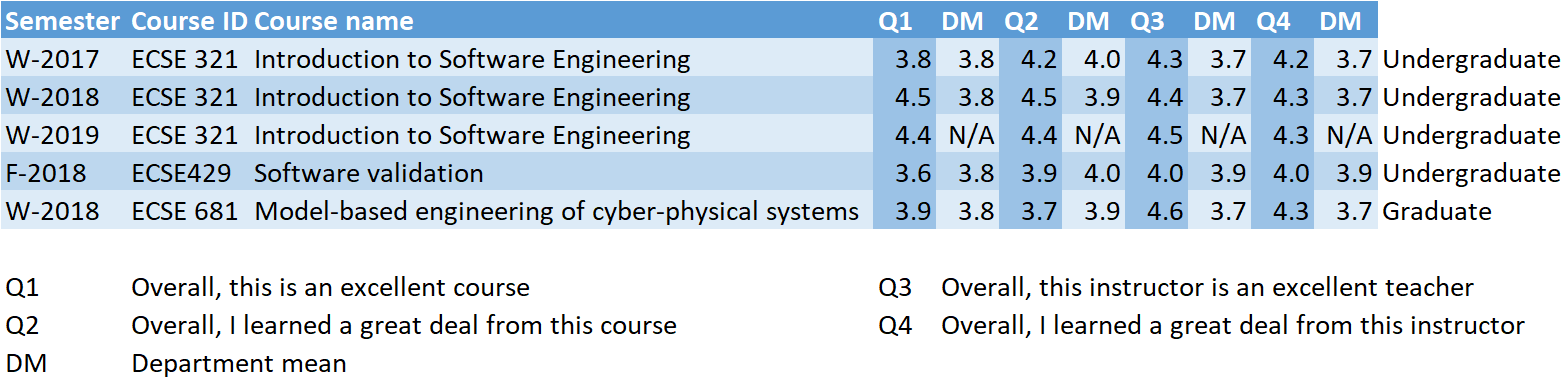
\includegraphics[width=\textwidth]{figures/TeachingEval}
%\caption{Results of course evaluations at McGill University}
%\label{fig:course-eval}
%\end{table}

\section{Services to Scientific Community}
%\lhead{Services to the Scientific Community} 
%\cvsubsection{Program Co-Chair}

%\subsection{Organizational roles in conferences}

\begin{refsection}[bib/pcmember.bib]
\newrefcontext{chref}
%\newrefcontext[labelprefix=CH]
\nocite{mise2019-chair,sle2016-chair,icmt2014-chair,fase2013-chair,amt2012-chair,grabats2010-chair,gtvmt2006-chair,grabats2006-chair}
\printbibliography[title=Program co-chair,heading=subbibliography]
\end{refsection}

\begin{refsection}[bib/pcmember.bib]
\newrefcontext{scref}
%\newrefcontext[labelprefix=SC]
\nocite{etaps2008-sc,etaps2013-sc,icmt2014-sc}
\printbibliography[title=Steering committee member,heading=subbibliography]
\end{refsection}

\begin{refsection}[bib/pcmember.bib]
\newrefcontext{loref}
%\newrefcontext[labelprefix=LO]
\nocite{icse2019post-chair,staf16ws-chair,staf2015ds-chair,staf2013-chair,models2012-chair,agtive2011-chair,sensus2009-lo,etaps2008-lo,models2007-chair,edcc2005-lo}
\printbibliography[title=Chair of organizing committees,heading=subbibliography]
\end{refsection}


%\subsection{Program Committee Membership}

\begin{refsection}[bib/pcmember.bib]
\newrefcontext{pcref}
%\newrefcontext[labelprefix=PC]
  \nocite{models2019-pc,ecmfa2019-pc,icse2019-pc,sefm2019-pc,mdeintel2019-pc,mpm4cps2019-pc,%
icse2018-pc,fase2018-pc,icmt2018-pc,ecmfa2018-pc,models2018-pc,securemde2018-pc,facs2018-pc,%
models2017-pc,fase2017-pc,icmt2017-pc,ase2017tools-pc,mise2017-pc,%
ase2016-pc,models2016-pc,ecmfa2016-pc,models2016ds-pc,icmt2016-pc,fmmdd2016-pc,%
ase2015-pc,models2015-pc,sle2015-pc,fase2015-pc,gam2015-pc,%
ase2014-pc,models2014-pc,fase2014-pc,vlhcc2014-pc,icgt2014-pc,%
  models2013-pc,ecmfa2013-pc,vlhcc2013-pc,%
  models2012-pc,ase2012-pc,ase2012tools-pc,icse2012tools-pc,vlhcc2012-pc,gtvmt2012-pc,%
  fase2012-pc,csmr2012-pc,ecmfa2012-pc,icmt2012-pc,icgt2012-pc,icgt2012ds-pc,%
  ase2011-pc,ase2011tools-pc,vlhcc2011-pc,gtvmt2011-pc,%
  models2011-pc,fase2011-pc,icmt2011-pc,ecmfa2011-pc,sofsem2011-pc,%
  mbsdi2011-pc,melo2011-pc,ictac2011-pc,ewdc2011-pc,%
  icgt2010-pc,ictac2010-pc,models2010-pc,fase2010-pc,icmt2010-pc,ase2010-pc,models2010edu-pc,gtvmt2010-pc,%
  models2009-pc,fase2009-pc,icmt2009-pc,ase2009-pc,gtvmt2009-pc,fm2009-pc,dsn2009-pc,%
  models2008-pc,icmt2008-pc,aramis2008-pc,gtvmt2008-pc,grabats2008-pc,icgt2008-pc,pngt2008-pc,%
  wapl2007-pc,models2007edu-pc,modeva2007-pc,atem2007-pc,sac2007-pc,gtvmt2007-pc,agtive2007-pc,%
  models2007edu-pc,%
  sac2006-pc,iwmec2006-pc,modeva2006-pc,atem2006-pc,gramot2006-pc,cmt2006-pc,gamma2006-pc,%
  fujaba2006-pc,icgt2006-pc,gtvc2006-pc,edcc2006-pc,icdcs2006-pc,%
  gtvc2005-pc,fujaba2005-pc,mtip2005-pc,gramot2005-pc,%
  grabats2004-pc%
  }
\printbibliography[title=Program committee membership,heading=subbibliography]
\end{refsection}


%\begin{refsection}
%\newrefcontext[labelprefix=SE]
%  \nocite{models2019-pc,ecmfa-2019-pc,icse2019-pc,%
%icse2018-pc,fase2018-pc,icmt2018-pc,ecmfa2018-pc,models2018-pc,securemde2018-pc,%
%models2017-pc,fase2017-pc,icmt2017-pc,ase2017tools-pc,mise2017-pc,%
%ase2016-pc,models2016-pc,ecmfa2016-pc,models2016ds-pc,icmt2016-pc,%
%ase2015-pc,models2015-pc,sle2015-pc,fase2015-pc,%
%ase2014-pc,models2014-pc,fase2014-pc,%
%  models2013-pc,ecmfa2013-pc,%
%  models2012-pc,ase2012-pc,ase2012tools-pc,icse2012tools-pc,%
%  fase2012-pc,csmr2012-pc,ecmfa2012-pc,icmt2012-pc,%
%  ase2011-pc,ase2011tools-pc%
%  models2011-pc,fase2011-pc,icmt2011-pc,ecmfa2011-pc,sofsem2011-pc,%
%  mbsdi2011-pc,melo2011-pc,%
%  models2010-pc,fase2010-pc,icmt2010-pc,ase2010-pc,modelsedu2010-pc,%
%  models2009-pc,fase2009-pc,icmt2009-pc,ase2009-pc,%
%  models2008-pc,icmt2008-pc,aramis2008-pc,%
%  wapl2007-pc,modelsedu2007-pc,modeva2007-pc,atem2007-pc,sac2007-pc,%
%  sac2006-pc,iwmec2006-pc,modeva2006-pc,atem2006-pc,gramot2006-pc,cmt2006-pc,gamma2006-pc,%
%  mtip2005-pc,gramot2005-pc%
%  }
%\printbibliography[title=Software Engineering]
%\end{refsection}

%\begin{refsection}
%\newrefcontext[labelprefix=VT]
%  \nocite{gam2015-pc,vlhcc2014-pc,vlhcc2013-pc,vlhcc2012-pc,gtvmt2012-pc,%
%  vlhcc2011-pc,gtvmt2011-pc,%
%  gtvmt2010-pc,%
%  gtvmt2009-pc,%
%  gtvmt2008-pc,grabats2008-pc,%
%  gtvmt2007-pc,agtive2007-pc,%
%  fujaba2006-pc,fujaba2005-pc,grabats2004-pc%
%  }
%\printbibliography[title=Visual Modeling Techniques and Tools]
%\end{refsection}

%\begin{refsection}
%\newrefcontext[labelprefix=FM]
%  \nocite{sefm2019-pc,facs2018-pc,fmmdd2016-pc,icgt2014,icgt2012-pc,icgt2012ds-pc,%
%  ictac2011-pc,icgt2010-pc,ictac2010-pc,%
%  fm2009-pc,%
%  icgt2008-pc,pngt2008-pc,%
%  icgt2006-pc,gtvc2006-pc,gtvc2005-pc}
%\printbibliography[title=Formal Methods]
%\end{refsection}


%\begin{refsection}
%\newrefcontext[labelprefix=DC]
%  \nocite{ewdc2011-pc,dsn2009-pc,edcc2006-pc,icdcs2006-pc}
%\printbibliography[title=Dependable Computing]
%\end{refsection}

%\begin{refsection}
%\newrefcontext[labelprefix=ED]
%\nocite{models2010edu-pc,models2007edu-pc}
%\printbibliography[title=Education]
%\end{refsection}


%\subsection{Other reviewing activities}

\begin{refsection}[bib/pcmember.bib]
\newrefcontext{dsref}
%\newrefcontext[labelprefix=DS]
\nocite{VargaJanos,Haussler,Oakes,AlBayati,Beyhl,GasconSamson,MarosiAttila,DeCarlos,Hegyhati,Vajk,Ciccozzi,Kalauz,Hildebrandt,Zombori,Guta,Siikarla,Lundkvist,Meszaros,Gergely,Vidacs,Hettel,Sipos,Lukacsy,Hajdara}
\printbibliography[title=Participation in PhD defense committees,heading=subbibliography]
\end{refsection}

\begin{refsection}[bib/pcmember.bib]
\newrefcontext{jrref}
%\newrefcontext[labelprefix=JR]
\nocite{sosym,jot,scp,ieee-tse,jss,ieee-sw,acm-tosem,sttt,ause}
\printbibliography[title=Journal reviews,heading=subbibintoc]
\end{refsection}

\begin{refsection}[bib/pcmember.bib]
\newrefcontext{ijref}
%\newrefcontext[labelprefix=IJ]
\nocite{cost,nwo,nserc,fct,fwf,mta,simi,york,stellenbosch,udem}
\printbibliography[title=International juries and academic evaluations,heading=subbibliography]
\end{refsection}

\newrefsection
\section{List of Publications}
\label{sec:publication-list}

%================================================
%\lhead{List of publications} 

\subsection{Summary of publication record}

\begin{table}[htb]
\begin{tabular}{@{}lllll@{}}
\toprule
\textbf{Publications} & \textbf{Lifetime} (20y) & \textbf{McGill} (3y) & \textbf{Student co-author} \\ \midrule
Journals & 47+1 & 9+1 & 30+1 \\ %\midrule
Book chapters & 9 & 1 & 6  \\ %\midrule
Conferences & 73 & 20 & 57  \\ %\midrule
Workshops & 33 & 3 & 20  \\ %\midrule
Other & 3 & 0 & 2  \\ %\midrule
Invited & 7 & 0 & N/A   \\ %\midrule
Edited & 11 & 2 & N/A \\ \midrule
Total & 182 & 35 & 115 \\ %\midrule
%PhD theses &  9 & 1 & All \\ \midrule
\bottomrule
\end{tabular}
\caption{Publication overview (Lifetime: 20 years, McGill: 3 years)}
\label{tab:publication-overview}
\end{table}


Number of citations: 6713 (as of August 14th, 2019 by Google Scholar) \\
%Number of citations: 3613 (as of November 30th, 2014 by CIDS 3.0) \\
%(of which in Scopus: 839, in MTMT: 1501) \\ 
%h-index (by CIDS): 31, g-index (by CIDS): 56, h-index (in MTMT): 26,\\
h-index (by Google Scholar): 43 \\
Source: \url{http://scholar.google.pt/citations?user=4Ya6dVoAAAAJ}  \\
DBLP: \url{https://dblp.uni-trier.de/pers/hd/v/Varr=oacute=:D=aacute=niel}  \\
%110 of my papers had a student co-author I supervised or co-supervised. \\
All papers which received a distinguished paper award had a student co-author \\
I had joint paper with 144 co-authors (DBLP data). \\


\paragraph{Choice of scientific venues.} 
When submitting a paper, I carefully select the target venue with the following considerations: 
\begin{itemize}[leftmargin=0.5cm]
\item My direct research area is model-based software and systems engineering where the top venues of the area are the \emph{IEEE/ACM MODELS conference} (Int. Conf. on Model Driven Engineering, Languages and Systems, previously known as the UML conference) and the \emph{Software and Systems Modeling} (Springer) journal. As such, many of my results have been published at these two venues. 
\item When a research result may be interesting for a broader software engineering audience, I may target major general-purpose software engineering conferences like \emph{ICSE} (ACM/IEEE Int. Conf. on Software Engineering), \emph{ESEC/FSE} (Foundations of Software Engineering),  \emph{ASE} (IEEE Automated Software Engineering Conf.) or \emph{FASE} (Fundamental Approaches to Software Engineering) and journals like \emph{IEEE Software}, \emph{Science of Computer Programming} (Elsevier), \emph{Software Tools on Technology Transfer} (Springer), \emph{IEEE Transactions on Software Engineering}, \emph{Automated Software Engineering} (Springer), \emph{Information \& Software Technology}, etc. I do not primarily check the impact factor (or other numerical classification) of such journals, but I rather verify if highly respected researchers regularly publish their.
\item I regularly publish results at smaller thematic conferences where I can get feedback from the top experts of a particular area, such as \emph{ICMT} (Int. Conf. on Model Transformations), \emph{ECMFA} (European Conf. on Modeling Foundations and Applications), \emph{VL/HCC} (IEEE Int. Symposium on Visual Languages and Human-Centric Computing), \emph{ICST} (IEEE Int. Conf on Software Testing, Verification and Validation), etc. 
\item When the formal foundations of our graph-based research needs to be presented, I regularly published at \emph{ICGT} (Int. Conf. on Graph Transformation).
\item Finally, we also published certain results at international workshops or electronic journals which provides an initial practice for my graduate students in scientific writing as well as an early feedback from senior experts of the field. 
\end{itemize}

\paragraph{Comments to publication list:} 
Names of students who worked under my supervision (or co-supervision) at the time of publication are marked with \textsuperscript{*}. The first author of a paper is frequently a graduate student who made the most direct contribution to the research. The last author is typically the supervisor who signs the research program. However, other policies of authorship are also common in case of cross-institutional collaborations (e.g. alphabetical order, mixed alphabetical, etc.). My own name is printed in \textbf{bold}, while my name is also \textbf{\underline{underlined}} for \emph{publications related to the research program I initiated when signing up for McGill University} (i.e. Stage 2 as explained in \autoref{sec:research-portfolio}). %As a consequence, I may exclude some papers when I already had a McGill affiliation or include a few papers without a McGill affiliation, but the the categorization of a few papers may not be unambiguous, but it still better reflects the role of the research program.

%Total number of papers: 166 \\
%Books and book chapters: 9 \\
%Peer reviewed (regular and electronic) journal papers: 45 \\
%Peer reviewed journal papers (incl. peer reviewed electronic journals): 35  (46) \\
%(incl. 10 in Software and Systems Modeling, Springer) \\
%Peer reviewed conference (+ workshop) papers: 69 (+33)  \\
%Refereed workshop papers: 31: \\
%Number of citations: 6572 (as of May 25th, 2019 by Google Scholar) \\
%Number of citations: 3613 (as of November 30th, 2014 by CIDS 3.0) \\
%(of which in Scopus: 839, in MTMT: 1501) \\ 
%h-index (by CIDS): 31, g-index (by CIDS): 56, h-index (in MTMT): 26,\\
%h-index (by Google Scholar): 41 \\
%Source: \url{http://scholar.google.pt/citations?user=4Ya6dVoAAAAJ}  \\
%DBLP: \url{https://dblp.uni-trier.de/pers/hd/v/Varr=oacute=:D=aacute=niel}  \\
%\url{http://cids.fc.ul.pt/cids_3_0/results.php?acc=3741130101140333046} \\
%\url{https://vm.mtmt.hu/www/index.php?AuthorID=10001355}
%ResearchNet: \url{https://www.researchgate.net/profile/Daniel_Varro/publications}
%\url{http://cids.di.fc.ul.pt/cids_3_0/results.php?acc=19271126111105329059}

\newpage

%============= Books and Book chapters ================
\nocite{fmi2004,nagl65-2010,bpel2sal-sensoria-book,sensoria-uml,SENSORIABook:AdvancesInGT,%
mdegt2005-ggzvvv,caise2011-revised,fmic2005-pv,fmhe2018}

\addtocategory{own}{fmi2004,nagl65-2010,bpel2sal-sensoria-book,sensoria-uml,SENSORIABook:AdvancesInGT,%
mdegt2005-ggzvvv,caise2011-revised,fmic2005-pv,fmhe2018}

\addtocategory{mcgill}{fmhe2018}


%============= Journal papers ================
\nocite{SCP2002,GRABATS2002j,GTVMT2003j,sosym2003-vpm,pp2003-as,FundInf2003-ghv,%
sosym2004-mc,gtvmt2004-gsv-j,gtvmt2004-vv-j,grabats2004-vfv-j,%
sosym2005-db,gramot2005-j,gramot2005-tax-j,%
sosym2005-bhtv,pngt2006-vv,gramot2006-j,hiradas2006-hvv,%
scp-2007,GT-VMT2007-hvv,gtvc2006-gkv,gtvmt2006-dpv-j,%
ijcsse08-kgv,Gonczy-safecert08,sosym2008-mtbe,%
Rath-sosym09,Bergmann-gtvmt09,%
Bergmann-sttt10,Gilmore-sosym10,eceasst2010-guided,eceasst2011-type,%
sosym2012-tools,sosym2011-cdt,sosym2011-csp,%
scp2015,ause2015,ist2015,sosym2016-trace,sosym2017-dsl,%
sosym2018-cep,sosym2016-viatra-invited,sosym2017-mondo,sosym2017-tb,act2017,%
sosym2019-mt,ieeesw2018,%
sttt-2019-cps,sttt-2019-div,sosym-2019-gamma} 

\addtocategory{own}{SCP2002,GRABATS2002j,GTVMT2003j,sosym2003-vpm,pp2003-as,FundInf2003-ghv,%
sosym2004-mc,gtvmt2004-gsv-j,gtvmt2004-vv-j,grabats2004-vfv-j,%
sosym2005-db,gramot2005-j,gramot2005-tax-j,%
sosym2005-bhtv,pngt2006-vv,gramot2006-j,hiradas2006-hvv,%
scp-2007,GT-VMT2007-hvv,gtvc2006-gkv,gtvmt2006-dpv-j,%
ijcsse08-kgv,Gonczy-safecert08,sosym2008-mtbe,%
Rath-sosym09,Bergmann-gtvmt09,%
Bergmann-sttt10,Gilmore-sosym10,eceasst2010-guided,eceasst2011-type,%
sosym2012-tools,sosym2011-cdt,sosym2011-csp,%
scp2015,ause2015,ist2015,sosym2016-trace,sosym2017-dsl,%
sosym2018-cep,sosym2016-viatra-invited,sosym2017-mondo,sosym2017-tb,act2017,sosym2019-mt,ieeesw2018,%
sttt-2019-cps,sttt-2019-div,sosym-2019-gamma} 

\addtocategory{mcgill}{sosym2017-dsl,sosym2018-cep,sosym2017-mondo,sosym2017-tb,act2017,sosym2019-mt,ieeesw2018,sttt-2019-cps,sttt-2019-div,sosym-2019-gamma} 


%============= Conference papers ================

\nocite{UML2002,ASE2002,ICGT2002-GHV02,ICGT2002-SC,%
esec03-bhtv,uml2003-tool,%
wicse2004-bhtv,GI2004,icgt2004-rsv,uml2004-meta,%
isas05-bvp,fase2005-eeltvv,vlhcc05-vsv,%
sac06-vtcl,sac06-plugin,isas2006-kvn,models2006-varro,icgt2006,%
agtive07-vhv,isas-2007-kv,sac2007-vb,%
icgt08-bhrv,Gonczy-mdwe08,icmt08-rbov08,Rath-vlhcc08,%
Bergmann-icmt09,Horvath-models09,Rath-models09,%
SEFM10-back-ann,models-2010-incquery,%
ase2011-dse,ase2011-mtslice,ase2011-tool,vlhcc2011,ecmfa2011,icmt2011,ServiceWave2011,%
models2012,ecmfa2012,icgt2012-ts,icst2012,tools2012,models2013,%
ase2014,models2014-iqd,models2014-stream,sle2014,csmr2014,%
icmt2015,icgt2015,%
fase2016-solver,fase2016-merge,icgt2016,MODELS2016-access,MODELS2016-bx,MODELS2016-metrics,%
esec-fse2017,models2017,adbis2017,icmt2017,%
icse2018-solver,icse2018-gamma,fase2018-diverse,fase2018-cps,models2018,vlhcc2018,nfm2018,models2018-tool,%
icse2019-tool,wf-iot-2019,models2019-wcet,models2019-systest} 

\addtocategory{own}{UML2002,ASE2002,ICGT2002-GHV02,ICGT2002-SC,%
esec03-bhtv,uml2003-tool,%
wicse2004-bhtv,GI2004,icgt2004-rsv,uml2004-meta,%
isas05-bvp,fase2005-eeltvv,vlhcc05-vsv,%
sac06-vtcl,sac06-plugin,isas2006-kvn,models2006-varro,icgt2006,%
agtive07-vhv,isas-2007-kv,sac2007-vb,%
icgt08-bhrv,Gonczy-mdwe08,icmt08-rbov08,Rath-vlhcc08,%
Bergmann-icmt09,Horvath-models09,Rath-models09,%
SEFM10-back-ann,models-2010-incquery,%
ase2011-dse,ase2011-mtslice,ase2011-tool,vlhcc2011,ecmfa2011,icmt2011,ServiceWave2011,%
models2012,ecmfa2012,icgt2012-ts,icst2012,tools2012,models2013,%
ase2014,models2014-iqd,models2014-stream,sle2014,csmr2014,%
icmt2015,icgt2015,%
fase2016-solver,fase2016-merge,icgt2016,MODELS2016-access,MODELS2016-bx,MODELS2016-metrics,%
esec-fse2017,models2017,adbis2017,icmt2017,%
icse2018-solver,icse2018-gamma,fase2018-diverse,fase2018-cps,models2018,vlhcc2018,nfm2018,models2018-tool,%
icse2019-tool,wf-iot-2019,models2019-wcet,models2019-systest}

\addtocategory{mcgill}{MODELS2016-access,MODELS2016-bx,MODELS2016-metrics,%
esec-fse2017,models2017,adbis2017,icmt2017,%
icse2018-solver,icse2018-gamma,fase2018-diverse,fase2018-cps,models2018,vlhcc2018,nfm2018,models2018-tool,%
icse2019-tool,wf-iot-2019,models2019-wcet,models2019-systest}

\nocite{dasc2010-hvs,Daboczi-AWSN2013,dasc2014}
\addtocategory{own}{dasc2010-hvs,Daboczi-AWSN2013,dasc2014}

%============= Workshop papers ================

\nocite{GRATRA2000,DDECS2000,WTUML01,%
edcc2002-svp,FMOODS2002,AGT2002,%GRABATS2002,GTVMT2002,
cbse03-bhtv,DDECS2003-tvp,csduml2003,%%grabats2004-vfv,gtvmt04-vv,gtvmt04-gsv,
mtip2005,%gramot2005-tax,gramot2005-adapt,gramot2006-vvs,
cmt2006,wsmate2006,dspd2006-rv,models2006-edu,%pngt2006-vv,gtvc2006-gkv,gtvmt06-dpv,
efts-2007-kgv,%GT-VMT2007-hvv,
gramot08-borvv,%Gonczy-safecert08,%Bergmann-gtvmt09,
SEFM10ToolDemo-back-ann,%eceasst2010-guided,
ocl2012,amt2012-query,
Kolovos-bigmde2013,Izso-bigmde2013,%
bigmde2014,cmseba2014,mpm2014,oss4mde2014,vao2014,%
staf2015-project,ttc2015,gemoc2015,%
BX2016,STAF-proj-2016,commitmde2016,%
commitmde2017,mdeintelligence2019}

\addtocategory{own}{GRATRA2000,DDECS2000,WTUML01,%
edcc2002-svp,FMOODS2002,AGT2002,%GRABATS2002,GTVMT2002,
cbse03-bhtv,DDECS2003-tvp,csduml2003,%%grabats2004-vfv,gtvmt04-vv,gtvmt04-gsv,
mtip2005,%gramot2005-tax,gramot2005-adapt,gramot2006-vvs,
cmt2006,wsmate2006,dspd2006-rv,models2006-edu,%pngt2006-vv,gtvc2006-gkv,gtvmt06-dpv,
efts-2007-kgv,%GT-VMT2007-hvv,
gramot08-borvv,%Gonczy-safecert08,%Bergmann-gtvmt09,
SEFM10ToolDemo-back-ann,%eceasst2010-guided,
ocl2012,amt2012-query,
Kolovos-bigmde2013,Izso-bigmde2013,%
bigmde2014,cmseba2014,mpm2014,oss4mde2014,vao2014,%
staf2015-project,ttc2015,gemoc2015,%
BX2016,STAF-proj-2016,commitmde2016,%
commitmde2017,mdeintelligence2019}

\addtocategory{mcgill}{commitmde2016,commitmde2017,mdeintelligence2019}

%============= Invited papers ================

\nocite{easst2006-etv,Wirsing-isola08,agtive07-toolcontest,models09-edu,csmr2012-invited,sofsem2016-invited,pame2015}
\addtocategory{own}{easst2006-etv,Wirsing-isola08,agtive07-toolcontest,models09-edu,csmr2012-invited,sofsem2016-invited,pame2015}

%============= Edited proceedings ================

\nocite{gtvmt2006,icgt2006-grabats,grabats2010,agtive2011,amt2012,fase2013,icmt2014,staf2015-ds,sle2016,staf2016-ws,mise2019}
\addtocategory{own}{gtvmt2006,icgt2006-grabats,grabats2010,agtive2011,amt2012,fase2013,icmt2014,staf2015-ds,sle2016,staf2016-ws,mise2019}

%============= End of own papers ================

\defbibfilter{books}{type=book or type=incollection or type=inbook}

%\defbibfilter{conf}{type=inproceedings and notkeyword={invited}}

\newrefcontext{bref}
\printbibliography[heading=subbibliography,filter=books,category=own,title=Books and Book Chapter]

\newrefcontext{jref}
\printbibliography[heading=subbibliography,category=own,type=article,notkeyword={workshop},notkeyword={invited},title=Refereed Journals incl. Electronic Journals]

\newrefcontext{cref}
\printbibliography[heading=subbibliography,category=own,notkeyword={invited},notkeyword={other},notkeyword={workshop},type=inproceedings,title=Peer Reviewed Conference Papers]

\newrefcontext{oref}
\printbibliography[heading=subbibliography,category=own,keyword={other},type=inproceedings,title=Other Conference Papers]

\newrefcontext{wref}
\printbibliography[heading=subbibliography,category=own,keyword={workshop},type=inproceedings,title=Refereed Workshop Papers]

\newrefcontext{iref}
\printbibliography[heading=subbibliography,category=own,keyword={invited},title=Invited Papers]

\newrefcontext{eref}
\printbibliography[heading=subbibliography,category=own,type=proceedings,title=Edited Volumes]

\chapter{Personal Statement}

After a successful academic career pursued in Hungary at the Budapest University of Technology and Economics where I got tenure in 2009 and promoted to a full professor in 2014, I joined the Department of Electrical and Computer Engineering at McGill University as a full professor in August 2016. Since 2015, I have held a research chair position in Hungary leaing a research program on cyber-physical systems as part of the prestigious and highly selective MTA Lendület program. 
This is an annually awarded in Hungary with only 12-15 researchers across all disciplines, and with only three past awardees in computer science since the foundation of the program in 2009. 

While this dossier dominantly presents details of my achievements after joining McGill University, I also provide a brief summaries about the pre-McGill period of my career. Furthermore, as a unique aspect of my research portfolio, I initiated and led an international research program involving more than 10 PhD students and several master's students both from Canada and Hungary.

\paragraph{Research.}
My main research area is \emph{model-based software and systems engineering} aiming for the design, analysis, optimization or deployment of traditional safety-critical systems as well as smart cyber-physical systems (CPS). My research contributed precise and scalable graph-based software techniques as foundations of design-time and run-time tools used in domains like avionics, automotive and various Internet-of-Things (IoT) systems. Since joining McGill University, we managed to substantially advance the state-of-the-art by (1) introducing distributed graph queries for runtime monitoring, (2) developing a novel family of automated model generator for domain-specific graph models, and (3) proposing various techniques secure collaborative modeling. Major ongoing multidisciplinary research carried out at McGill University aims to support the digital multidisciplinary analysis and design optimization platform.

I have been continuously aiming to publish my research results at top scientific conferences and journals of model-driven engineering (my direct research area) or alternatively, at general software engineering venues. In my career, I have published 171 papers (34 since joining McGill) including 47 papers in peer-reviewed journals (10 at McGill), and 73 peer-reviewed conference papers (20 at McGill). I have published several papers at a large variety of major scientific venues of my research area including IEEE/ACM sponsored conferences of software systems such as e.g. MODELS, ICSE, ASE, ESEC/FSE and top journals (e.g. Software and Systems Modeling, IEEE Software, Software Tools on Technology Transfer, Science of Computer Programming, Information and Software Technology). My papers received over 6710 citations (according to \href{https://scholar.google.ca/citations?user=4Ya6dVoAAAAJ&hl=en}{GoogleScholar}) with a Hirsch-index of 43. As of today, I am the most cited software engineering researcher at McGill University.  

As a recognization of our research, \emph{seven papers} co-authored by my graduate students and myself received \emph{Best / Distinguished Paper Awards} at leading conferences (4x at MODELS, 1x at ASE 2011, 1x at CSMR-WCRE 2014 and 1x ETAPS 2018). Three of these papers were published after joining McGill University. Furthermore, \emph{two 10-year Most Influential Paper Awards} for our pioneering work on generic and meta-transformations (awarded at IEEE/ACM MODELS 2014) and benchmarking graph transformation tools (recognized at IEEE VL/HCC 2016).

I gave a total of 35 invited talks (10 talks since joining McGill) at international graduate schools, research seminars, at various companies (e.g. Ericsson, Embraer, Rockwell Collins) and research institutes (e.g NASA Jet Propulsion Lab, SRI International) - 10 of these talks were delivered after joining McGill. I was invited to give a keynote talk at leading software engineering conferences (CSMR 2012 and SOFSEM 2016), and a plenary talk at MODELS 2014 upon receiving the Most Influential Paper award. Moreover, I gave keynote talks at national conferences (CSER 2017 in Canada and CSCS 2016 in Hungary) and at numerous workshops. I gave a total of 9 talks and 4 tutorials at international summer schools.% (DSM-TP, SERENE, SENSUS). 

I was successful in securing competitive research funding on a Canadian, European and Hungarian level by acquiring an equivalent of over 4.5 million CAD for my own research. This includes competitive funding over 600,000 CAD in Canada (after joining McGill) along projects in the NSERC Discovery Grant program and the Collaborative Research and Development program with Siemens. Prior to succeeding as a Lendület research chair at the Hungarian Academy of Sciences, my ERC Starting Grant project CERTIMOT (in 2009) went through to the final round, and it was recommended for funding, but become out of budget, but it still received partial national funding later. I acted as the site leader (or research director at BME) of five collaborative European projects.% in the FP6 and FP7 framework in the field of service-oriented computing (SENSORIA), avionics (DIANA), evolving secure systems (SecureChange), transport (E-Freight) and scalable model-driven engineering (MONDO). 
I was the PI of industrial projects with Embraer, Ericsson and Nokia. I am a three-time recipient of the IBM Faculty Award.

\paragraph{Student supervision.}
I have been the main supervisor of 11 PhD students and a co-supervisor for 6 PhD students with 11 successful defenses up to now. Seven of those PhD students had a McGill affiliation (as a PhD student or as a graduate research trainee at McGill). I have also supervised 5 MEng students and 38 undergraduate students and at McGill University (with career total of 28 MSc/MEng students). 115 of my research papers have at least one student co-author I supervised or co-supervised (with 32 out of 34 papers after joining McGill). My graduate students successfully competed in various doctoral research competitions organized at top international conferences achieving twice a 1st prize and once a 3rd prize after I joined McGill. 
%Previously, I was selected as (the youngest ever) Distinguished Tutor, a bi-annual national prize requiring 10 years of successful tutoring. 
In 2017, I was the first ever recipient of the Csanád Imreh Award where a single award is given bi-annually to scientists in the field of computer science below the age of 41. 

\paragraph{Service.}
Since joining McGill University, I was invited to serve in various senior organizational roles at major international conferences, such as the program co-chair (SLE 2016, MiSE 2019), posters co-chair (ICSE 2019), program board member (MODELS 2016 and 2017), steering committee member (ICMT) or editorial board member (SoSyM, JOT). I served on the program committee of major international conferences of my field (including e.g. ICSE, MODELS, ICMT, ECMFA). At ICSE 2018, I received an \emph{ACM Distinguished Reviewer} award for my thorough reviews. I served as an external reviewer for various international projects and grants in 4 countries. Previously, I served as the program co-chair of FASE 2013, ICMT 2014, general chair of AGTIVE 2011 and STAF 2013, and the local organizing chair of ETAPS 2008 and EDCC-5, and served on the program committee of over 100 conferences and workshops.

At McGill University, I have served on 8 different committees for the ECE Department and 2 faculty-level working groups. For example, as a member of the Search Committee of the ECE Department in 2018 and 2019, I evaluated application packages of hundreds of applicants. Since 2018, I have been an elected representative of the Faculty of Engineering for the Council of Graduate and Postgraduate Studies (CGPS). In addition, I have been serving as an internal or external examiner for 5 PhD theses after joining McGill (with a career total of 24 PhD thesis reviews) in four different countries.


\paragraph{Teaching.}
Within the five courses I taught at McGill University, my most significant achievements were in the ECSE 321 Introduction to Software Engineering course where I successfully modernized the software technologies, brought in real customers for the complex software engineering project, redeveloped tutorials, and initiated the development of an autograder software for objectively evaluating technology assignments of students. Students are very supportive of my teaching style as 90\% of my instructor-specific course evaluation scores are over 4.0 (out of 5.0). Finally, I also gave 3 invited lectures and 2 tutorials at the international DSM-TP summer school. I also serve as the program director of the upcoming software engineering co-op program (expected to start in 2020) where undergraduate students will need to spend four compulsory internship terms at companies. In that role, I have been working on the key policies, guidelines, student and employer evaluation forms related to the co-op terms since Fall 2018.

%Teaching experience and course development. Since 2003, I have been involved in the development of 10 university courses on different levels (for BSc, MSc and PhD students) first at BME and then at McGill University. I was in charge of developing an undergraduate specialization on Systems engineering now an accredited curriculum at BME. I have been lecturing regularly for 70-120 on different levels (and occasionally for 200+ undergraduates). At McGill, I am the program director for the upcoming software engineering co-op program where undergraduates spend compulsory internships at companies as part of their curriculum. I am a co-author of a (Hungarian) textbook and I was an invited panelist at MODELS 2009 Educators’ Symposium. 

\paragraph{Experience in software industry.}
In 2013, I co-founded IncQuery Labs, an innovative Hungarian company, together with the first generation of my former PhD students (who are current executives of the company). I played a major role in acquiring the first large-scale projects e.g. with Ericsson and TeqBall and participating in its first European project OpenCPS. In 2016, the company received a 3rd place on the Deloitte Rising Star list as the fastest growing Hungarian company in Central Europe. In 2018, I was representing the company as part of the SysML 2.0 standardization in the Object Management Group. 

As further industrial experience, I was the founder and (until 2016) the main strategist of the open source VIATRA model query and transformation framework (used at Thales, Ericsson, NASA JPL, Airbus ThyssenKrupp Presta, several automotive tool vendors and in open tools like Capella, Artop or Papyrus) and a co-founder of MASSIF, a Matlab Simulink Integration Framework for Eclipse (used e.g. at INTECS, CEA, MapleSoft MBSE).  These projects started as research prototypes funded by research projects, and they gradually evolved to an industrial tool now maintained by IncQuery Labs Ltd.

%Previously, I was Vice President of Research at OptXware Ltd, a Hungarian spin-off company. I participated in a national project supporting the development of product family of service dependability and optimization.  After developing an Eclipse based toolkit for AUTOSAR, the company was partially acquired by a large international automotive company. I was one of the company representatives during the acquisition talks.

\documentclass[a4paper,11pt]{report}
%\documentclass[a4paper,12pt]{article}
%\usepackage[backend=biber,sorting=ydnt,maxnames=18,giveninits=true,labelnumber=true,defernumbers=true]{biblatex}
%\usepackage[backend=biber,sorting=ydnt,maxnames=18,giveninits=true]{biblatex}
%\usepackage[bibstyle=publist]{biblatex}
\usepackage{xstring}
\usepackage{url}
\usepackage{booktabs}
\usepackage{hyperref}

\usepackage{titlesec}
\titlespacing*{\section}{0pt}{12pt plus 1pt minus 0.5pt}{6pt plus 0.5pt}
%\titlespacing*{\subsection}{0pt}{5.5ex plus 1ex minus .2ex}{4.3ex plus .2ex}

\titlespacing*{\paragraph}
{0pt}{3pt plus 1pt minus 0.5pt}{3pt plus 2pt minus 0.5pt}

\usepackage{enumitem}
\setlist{nosep}

\usepackage{tcolorbox}

\usepackage{fontspec}
\setmainfont{Cambria}
\setsansfont{Calibri}

%\setlength{\itemsep}{0pt plus 1pt}
%\setlength{\itemsep}{0pt}
%\setlength{\topsep}{0pt}
\setlength{\parskip}{3pt plus 0.5pt minus 0.5pt}
%\setlength{\beforeskip}{3pt}


%\usepackage[scale=0.85]{geometry}
\usepackage[scale=0.85]{geometry}

\geometry{
 a4paper,
 total={170mm,257mm},
 left=20mm,
 top=20mm,
 }

%\assignrefcontextkeyws[labelprefix=C]{C}
%\assignrefcontextkeyws[labelprefix=J]{J}

\usepackage{fancyhdr}
\pagestyle{fancy}\lhead{Teaching Statement} \rhead{May 2019}
\chead{{\bf Dániel Varró}} \lfoot{} \rfoot{\bf \thepage} \cfoot{}

%\title{Teaching Portfolio}
%\author{D\'aniel Varr\'o}
%\date{August 2019}

\begin{document}
%\maketitle
\setcounter{page}{17}

\vspace{12pt}

\chapter{Teaching Statement}

\begin{tcolorbox}[title=Executive Summary of Teaching Activities]
As a \emph{course instructor}, a main philosophy of mine is that a software engineering related course should \emph{simultaneously teach conceptual foundations and cutting edge software technology}. Without the former, a course becomes empty - without the latter, a course becomes irrelevant. I am dedicated to bring \emph{realistic engineering challenges} frequently with real customers to a course that \emph{facilitate collaboration} within and between student teams while they acquire the new concepts and technologies. I regularly use various  means of \emph{active learning} to make my lectures lively. Furthermore, I always wish to maintain an \emph{inclusive atmosphere} even for a \emph{diverse and international audience}. 
\vspace{3pt}

As a \emph{supervisor} who actively collaborates with his graduate students with in-depth discussions, my goal is to continuously \emph{strive for excellence} both in engineering tasks as well as in publications while my graduate students are gradually becoming more and more \emph{independent researchers with critical thinking}.  My students typically undertake deep research tasks which go well beyond the state-of-the-art. As a further characteristic, many of our past \emph{results are simultaneously precise and scalable}, and it has been actively \emph{used in an industrial setting}. Active investment in research prototype tools help my students become \emph{excellent software engineers and architects}.
\end{tcolorbox}


\section{Statement on Teaching and Supervision Philosophy}

\subsection{My philosophy as a course instructor}

My passion for teaching dates back to my first experience as a teaching assistant in 1999 at BME. Since then, it has been 
extremely energizing for me to guide talented and hard-working students on their path towards excellence to succeed as 
software engineering professionals. For me, teaching is more about sharing my experience and expertise rather than the 
actual act of lecturing. For this this purpose, I typically combine lectures with games, interactive sessions, individual 
assessment and group work. 

\paragraph{From software engineering students to professional software engineers}
As a course instructor, my main objective is to guide students to become professional software engineers. This is very 
challenging, since by the time a graduated student becomes a software engineering professional, he or she needs to solve 
vaguely defined problems independently, work effectively in teams, in a rapidly changing technical and socio-economical 
context - in addition to the deep knowledge of software engineering concepts and technologies. I find it very important that 
students face these challenges already in some of their university courses (instead of dealing only with well-defined 
problems and idealized solutions). In a software engineering course, I frequently position myself as a mentor or a product 
manager: I am ready to help students find solutions to their problems, but they should make serious attempts to find 
solutions first on their own by learning how to use the vast amount of information available on the Internet (e.g. tutorials, 
technical forums, mailing lists). 

\paragraph{Learning by example}
There are typically multiple solutions to any given software engineering problem, and students need to be able to evaluate 
the advantages and disadvantages of a particular solution. For that purpose, they need to be exposed to many examples 
ranging from toy examples demonstrating one aspect of the problem to complex case studies where many problems need to 
be tackled at the same time. Students are exposed to different kinds of hands-on activities such as tutorials, tools, 
assignments, projects, etc. to ensure a balanced development of their software engineering skills. Also in my lectures, I 
postpone abstract definitions during my lectures to the point when the main concepts are sufficiently demonstrated by small 
examples first.

\paragraph{Interactive classroom for active learning}
%Maintaining the attention of students during lectures can be a challenging task.  %Moreover, 
I regularly intertwine lecturing with different sort of activities to make the classroom more interactive. I frequently use 
various \emph{best practices of active learning} during my lectures (e.g. bug hunts on ill-formed software, various games 
and quizzes, small challenges discussed in small groups). I often \emph{demonstrate the practical relevance of concepts 
using real-world examples} and industrial case studies sometimes presented by industrial collaborators within invited 
lectures. 

\paragraph{An all-inclusive classroom}
I am dedicated to make my courses inclusive to students of any diversity group, social or technical background. Even in case of a lively discussion, nobody should ever be humiliated or personally attacked. I actively push students to interact with fellow students with a very different background. I also regularly give advice to problematic teams to carry out groupwork more effectively. In order to reduce stress caused by high course workload, I do not impose penalties on late submission for the first time, and I may adjust the requirements of deliverables when needed. 


\paragraph{Use of modern software technologies}
I strongly believe in \emph{teaching software engineering concepts in the context of modern software technologies} and 
project management frameworks. Although software technologies are evolving rapidly, job advertisements dominantly seek 
for students based on their technological background. When a modern software engineering course needs to use software 
technologies widely used in the industry, motivating students becomes much easier - as they know that what they learn can 
directly appear in their CV. Most of \emph{my courses are complemented with tutorials} on key technologies (e.g. on multi-
tier web applications or software quality assurance techniques) actively co-developed by my graduate students which also 
provides a first teaching experience for them. Online tutorials frequently serve as a reference document for students while 
tackling their complex group projects.

\paragraph{Project-based courses}
Most of my courses are project-based. Students need to invest significant amount of work in completing a \emph{team 
project} in groups of 3-5 persons. I assign a \emph{complex software/systems engineering challenge ideally proposed by a 
real customer}. As a result, students have to apply the concepts and technologies taught in the course in a realistic setting, 
which results in a much deeper learning experience. Furthermore, students can use their projects as reference work after 
the completion of the course in job interviews. 


\subsection{My philosophy as graduate supervisor}

As a supervisor of graduate students, I feel an increased level of responsibility as by the end of several years with collaborative research, I have established very strong technical and personal ties with my graduate students. When I take somebody as a PhD student, I normally clarify his or her planned career path after the completion of the PhD (e.g. taking an academic or an industrial path) to ensure a personalized treatment. 

I am very proud to be the main supervisor of 7 successful PhD defenses and the co-supervisor of 4 successful PhD defenses. Three of my former students have (part-time) academic positions at BME while four of them has been co-founders of the successful Hungarian start-up company, IncQuery Labs. Ltd. Others are in leading technological positions in large industrial companies (e.g. ThyssenKruppPresta).

\paragraph{Selection of students}
I normally prefer guiding graduate students from the beginning of their Master's studies to their end of their PhD. I regard their Master's thesis as a probation period (1) to judge if the student is capable of doing research work independently, and (2) to ensure that there is no personal misfit between the graduate student and myself, and (3) to confirm that they are strong team players to collaborate with others. Having strong mathematical and abstraction background and strong software engineering skills is also required prior to starting PhD studies. Having strong writing skills is a plus, but I am quite effective in helping students improve their scientific writing skills. 

\paragraph{Solve challenging problems vs. publications}
I regard publications as bi-products of outstanding research carried out to solve a complex, and highly uncharted software engineering problem. My graduate students do not only publish papers for the sake of their CV, but they use publications as a means to report about their deep scientific results in software engineering. For me, publishing one paper that reports how a problem is actually solved is more valuable than writing three papers which gradually progress towards a solution. I feel strong at motivating students to start exploring highly uncharted research areas, and the lack of significant previous work in a certain area frequently boosts the motivation of talented students. 
When publishing results, I help identify typical errors made by students due to their lack of expertise in scientific writing which helps them achieve early successes. Then I gradually let them act more and more on their own to gradually gain independence in writing by the time they defend their PhD. 

\paragraph{Industrial relevance}
Normally, I prefer that my graduate students find research problems that either directly address industrial needs, or at least, in case of highly uncharted areas, there would be a strong industrial need for the missing solution. Typically, I help them select their first 1-2 challenges, and after that, they can start exploring new research lines on their own. 
My students have regularly participated in long-term industrial collaborations in research intensive tasks. 

\paragraph{Open source projects}
Several PhD projects have been grouped around complex open source projects and demonstrators which have been successfully maintained and continued well beyond the lifetime of a single PhD project. I strongly believe that such open source projects facilitate team work between students and provide a greater visibility of their research for the general public. In fact, our open source projects have been repeatedly used by several research groups as a baseline for comparing their results. 

\paragraph{Public benchmarks for open science}
Since 2005, we have been developing several public benchmarks to allow an in-depth comparison of different software algorithms and tools to a given research challenge. This helps graduate students learn what others did in a particular field by trying out and experimenting with their tools. Moreover, it also helps them find gaps in the state of the art, and thus they have more confidence in the novelty of their own algorithms. Finally, it also promotes the open science initiative to ensure that research results can be reproduced outside their original context.

%guiding 




%\section{Teaching Responsibilities}
%Starting as a teaching assistant in 1999, I have been involved in teaching at various levels as a full-time staff member at the Budapest University of Technology and Economics (BME, lecturing dominantly in Hungarian) between 2003 and 2016 and since then at McGill University (Canada, lecturing in English). The list of all courses I taught are listed in my CV (page \ref{xxx}).

\section{Executive summary of past teaching activities at BME}

Before joining McGill University in 2016, I already had a long track record of teaching and course development since my early PhD studies. Altogether, I developed or co-developed 7 courses (3 undergraduate, 3 MSc-level, 1 PhD-level) and taught  over over 25 editions of those courses. Below, I provide a brief executive summary only about my most significant activities at BME. 

\paragraph{Undergraduate-level teaching}
I contributed to the development of a course on \emph{Formal methods} (with 300+ students each year) since the beginning of the course in 2001 and giving several guest lectures between 2004 and 2006. I also contributed three chapters in the new textbook of the course (in Hungarian).  Moreover, I was a key contributor and strategic founder of an \emph{undergraduate curriculum on Systems Engineering}.  I was major promoter and initiator of the development of an \emph{autograding software tool} (implemented by my graduate students) and subsequently used in the \emph{Systems Modeling} undergraduate course for over 5 years by now with 600+ students where each student could receive an individual technical assignment. 

In a project manager role, I participated in introducing virtual labs over educational cloud (using Apache VCL) at our faculty for the first time in Hungary which received a \href{https://inf.mit.bme.hu/en/news/2014/02/tempus-stem-call-apache-vcl-based-labs-won-prize}{TEMPUS STEM Award} in 2014. 

\paragraph{Graduate-level teaching}
At BME, I developed a course on \emph{UML-based modeling and analysis} which ran between 2003 and 2009 for 70-80 graduate (MSc) students. \emph{Several teaching assistants of the course were former students} of the course who \emph{voluntarily came back from industry to help the course}, which was a highly unusual way of teaching in Hungary. Between 2009-2016, I ran a course on “Model-driven software/systems development” (twice in English) with 15-20 students each year. I also actively contributed to start the first ever Hungarian university course on \emph{Eclipse based technologies} in 2005. I was also involved in several industrial trainings on these topics. I have been running a PhD seminar on the \emph{Foundations of Model-Driven Engineering} between 2004 and 2014 (with 5-8 students each year). In 2009, I was \emph{invited as a panelist at the Educators' Symposium} of the MoDELS conference, the main scientific venue of my field. 


\section{Courses Taught at McGill}
Since 2016, I taught five editions of three different courses at McGill University: ECSE 321: Introduction to Software Engineering (taught 3x), ECSE 429: Software Validation (1x), ECSE xxx: Critical Systems (1x, under temporary course code: 681) . Below, I provide an overview of the most significant course development activities are carried out in the respective courses. 
Since I only offered the ECSE 321 course more than once at McGill prior to submitting my tenure dossier, my primary focus will be on that course where the impact of my course development activities have been most apparent - and where I had chances to reflect to students' feedback I received in course evaluations.  

As the important success story for the undergraduate courses I taught (ECSE 321 and ECSE 429), I successfully integrated various cutting-edge software technologies to those courses and involved real customers/software in team projects. As a result, \emph{several students succeeded in getting summer industrial software engineering internships based solely on course material}. The graduate course, which teaches concepts and standards of model-based systems engineering, has a similar success story. Furthermore, I successfully led the development of an auto-grader software framework which can help automatically evaluate software-related assignments of students by using test cases and exploiting modern cloud-based software technologies.

\subsection{ECSE 321: Introduction to Software Engineering (Undergraduate)}
I took over this undergraduate course from Prof. Mussbacher and offered it in alternation with Prof. McIntosh who modernized many concepts taught in the course. The course covers the entire lifecycle of a modern software project including requirements engineering, domain modeling, test-driven development, continuous integration and software configuration management in the context of a group project and individual assignments. The 75-100 students of the course must have taken 1-2 previous programming courses prior to enrolling to this course. Below I highlight major developments of the course where my own initiative was predominant to improve the industrial relevance of the course, which received very positive feedback from McGill undergraduates. 
% and (2) to limit grading efforts with increasing enrollment. 

\paragraph{Modernization of software technologies and team project}
It was apparent from student feedback I received in the Winter 2017 edition of the course that the software technologies are outdated, and the students do not feel they learn modern material despite the modern concepts. Moreover, students had to develop a smaller system to three different platforms, thus they were not imposed to face integration problems which are characteristic to most modern software.

Therefore, since Winter 2018, I took the initiative and modernized the entire underlying software stack used within the course including the following specific major improvements:
\begin{enumerate}
\item The team project should \emph{develop an integrated multi-layer web application} with separate backend (i.e. services and database) and different graphical user interface frontends (mobile, web). 
\item I changed the Java-dominated technological stack to include \emph{heterogeneous technologies} including a modern web technologies (like HTML5, JavaScript or Vue.js), a modern backend technology (JavaSpring, RESTful API), and Gradle for build automation. I also included respective programming concepts such as asynchronous method calls or promises. 
\item I introduced a proper underlying relational database technology on top of an object persistence layer using the standard Java Persistence API. I developed respective lecture material to cover the basic concepts of relational databases (as students take the Database course later) and the standard \emph{object-relational mapping}.  
\item While Montreal is a major aerospace hub, the existing courses of the software engineering curriculum failed to offer specific insights in engineering critical systems. Therefore, I developed lectures on \emph{platform-based design in systems architecture} as well as the \emph{foundations of fault-tolerant systems}.
\end{enumerate}

Since the theme of the software engineering team project was different in every year, students could decide if they wish to open their GitHub repositories that stored the source code of their projects after the completion of the course. Many teams opted for an open repository and \emph{students started to use their ECSE 321 project as a reference work during interviews of summer internship}. This is clear indication of the industrial usefulness and practical effectiveness of the course as a result of the changes above. 

\paragraph{Involving real customers in team projects}

To better motivate students, I put extra emphasis on providing real challenges for the complex software engineering project carried out by teams. Therefore, I selected project themes where McGill employees could serve as real customers. Those customers participated in requirements engineering sessions where students could ask questions to clarify the scope of the project. Moreover, these customers also attended (and graded) the final student presentations and the final software artifact.
\begin{itemize}
\item In Winter 2018, student teams had to develop a software application to manage and supervise the trees in Montreal and calculate various forecasts for evaluating sustainability attributes. Many details of the project were proposed by Prof. Andrew Gonzalez, Prof. Kevin Manaugh and Prof. David Wachsmuth who offered their continuous involvement.
\item In Winter 2019, student teams had to develop an application to help manage co-op programs (i.e. curricula with compulsory industrial internship) at McGill University. In this case, Ms. Lorraine Donald (Industrial Liason Associate and future administrative coordinator of the upcoming software engineering co-op program) offered continuous help during the project. Moreover, final presentations of student teams were also attended by various employees at the Faculty of Engineering.
\end{itemize}


\paragraph{Redevelopment of tutorials: contents and technology}
As a consequence of the above initiative, the \emph{sample project as well as the technical contents of the tutorials of the course had to be redeveloped from scratch} which I carried out together with Márton Búr, my PhD student (with further initial help from my graduate students at BME, Gábor Szárnyas and Oszkár Semeráth). This was a major investment since the total length of the PDF version of the material was 75-100 pages. 

To improve the maintainability of tutorial materials, I promoted to host those tutorial materials on GitHub and continuously compile changes into a new version of the document available both in HTML and PDF formats (see e.g. 
\href{https://mcgill-ecse321-winter2019.github.io/EventRegistration-Tutorials/}{ECSE321-W2019}, 
\href{https://mcgill-ecse321-winter2018.github.io/EventRegistration-Tutorials/}{ECSE321-W2018}, 
\href{https://ecse321-winter2017-mcgill.github.io/EventRegistration-Tutorials/}{ECSE321-W2017}). As such, even the tutorials of the course actually used the same software technologies (Gradle, Github, TravisCI) taught by the course. 



\paragraph{Auto-grader for individual software technology assignment}
To assure that all students taking the course successfully learned not only the core concepts but also the key software technologies, a programming assignment has already been an integral part of the course where students had to develop a small-scale web application using the same technologies as in the large-scale group project. This assignment had to be carried out by the students either in pairs (in 2017 and 2018) or individually (in 2019). 

However, the evaluation of these individual assignments has been very laborious and somewhat subjective and error-prone. Therefore, I took the initiative to develop an auto-grader framework that could automatically evaluate student submissions by running predefined test cases. The key concepts of the auto-grader framework are the following:

\begin{itemize}
\item Each student needs to develop a unique combination of software features by extending a baseline web application made available to them as a starting point. All development needs to be done in an individual (private) GitHub repository of the student (identified by their McGill IDs). The individual specification of the assignment is also generated automatically for each student. 
\item The auto-grader evaluates student submission by running a dedicated test suite. The Instructors need to develop the superset of all test cases from which the auto-grader selects the ones required for the features addressed by the specific student. 
\item The 80\% of the test cases are made publicly available to students so that they can use them as a reference while developing their solution. The remaining 20\% of the test cases were only included in the official grading process. 
\item The actual grading is carried out as part of a continuous integration process, which automatically builds the student project, then executes the relevant set of test cases, and finally reports the evaluation in a separate GitHub branch.
\end{itemize}

The auto-grader has been successfully used in Winter 2019, but several colleagues at my department has expressed there interest in potetially adapting the framework to their course. 

\paragraph{Undergraduate students as project mentors}
With the help of the Tomlinson Engagement Award for Mentoring (TEAM), I systematically involved excellent undergraduate students in the next edition of the ECSE 321 course. A total of six TEAM mentors (in 2018 and 2019) successfully helped team projects to overcome the difficulties of integrating various software technologies. Moreover, they also helped develop the auto-grader framework. While the TEAM award is on a nomination basis, several undergraduates have indicated to volunteer for the next year, which clearly demonstrates the positive impact of this change.


\subsection{ECSE 429: Software Validation (Undergraduate)}

I gave this undergraduate course in Fall 2018 for over 120 students - most of who were taking this course just before their graduation. The course covers various techniques of software quality assurance including testing, static analysis and formal verification. The students of the course need to complete a complex software testing project (in teams) as well as individual testing assignments and three quizzes.

Since the lecture material of the course has been recently redeveloped (by Prof. Mussbacher), I built upon and reused significant amount of existing course material. Since the software technologies used within the course were outdated, my primary goal was to increase the practical and industrial impact of the course by the following initiatives:

\begin{enumerate}
\item The \emph{tutorials of the course have been redesigned almost from scratch} (with contributions from the two teaching assistants, Márton Búr and Mathieu Boucher). New material included the introduction of code reviews, continuous integration, modern static analysis tools (SonarQube, Infer), automated test case generators (EvoSuite), various frameworks for integration testing as well as end-to-end testing Android applications, model-based testing tools. I adapted the use of GitHub for hosting the \href{https://mcgill-ecse429-fall2018.github.io/Tutorial-Lecture-Notes/}{material of the tutorials}, which allows that corrections can be immediately published to the live material (without extra manual document upload). 

\item As being of utmost importance in modern software quality assurance, I \emph{developed course material related to code reviews and and static analysis techniques} as part of the lectures and introduced an extra deliverable for the team project. To further increase practical relevance, the introductory materials of software quality assurance and testing has been aligned with contents and recommendations of the International Software Testing Qualifications Board (ISTQB) for foundation level certification.

\item Within the complex team project of the course, \emph{student teams had to test a real open source Android application} (Blokish game). Although the suitability of this very project was criticized by students, they were simultaneously enforced to understand and handle the imperfections of real software projects, which is frequently the case in real software projects. 

\item To avoid the laborious work of grading the three individual quizzes with an increased number of enrolled students, I \emph{changed the former closed-book in-class quizzes into an open-book, online quizzes} evaluated semi-automatically using existing support in MyCourses. Students had to complete each quiz in 75 minutes within a 6-hour time-frame, which gave them extra flexibility to avoid clashes of midterm exams with other courses, and in general, it reduced the perceived stress level. 
\end{enumerate}

\subsection{ECSE xxx/681: Critical Systems (Graduate)}

I proposed and \emph{developed a new graduate course on Critical Systems} to provide an overview of main challenges and activities in the design and assurance of critical software-intensive cyber-physical systems (CPSs). The first part of the course is dedicated to the core concepts, languages and techniques of model-based systems engineering used for designing such systems while covering key concepts like safety cases, traceability, viewpoints of system architecture, design space exploration, etc. In this first part, students carry out a complex design project using standard modeling languages (like SysML, Capella) and simulation tools in the context of a cyber-physical system or Internet-of-Things application. This first part is complemented with in-class tutorials and modeling workshops to help students effectively use complex industrial systems engineering tools.

The second part of the course is dedicated to assurance critical CPSs to guarantee the safe behavior of such systems by discussing a wide range of design-time and run-time assurance techniques. In the second part, students familiarize themselves with research results used for the assurance of such systems including various approaches of verification and validation (V\&V). The end of the course is dedicated to recent research challenges for the safety assurance of autonomous systems driven by machine learning and other AI techniques. These research-related contents are close to my own research area, thus student presentations of various research topics normally involve lively and deep discussions. 

I offered the first edition of the course (under a temporary course code) in Winter 2018 for 18 graduate students. As an extra research component for this first edition, students had to assemble a survey presentation of a research topic by categorizing over 15 papers. The official approval of the course is ongoing, and it is expected to be completed in Fall 2019. 


%\paragraph{Undergraduate-level courses.}

%At \emph{McGill University}, I was the instructor of a course on \emph{Introduction to Software Engineering} for three times with 75-95 students in 2017-2019 and for a very diverse and international audience. In all three editions, I received an average score between 4.2-4.5 (out of 5.0) for all course evaluation questions related to me as instructor, which was significantly over the department average (by an average of 0.6). In 2018, I significantly modernized the technological background of the course – which now teaches modern software engineering principles and architectures in the context of modern software technologies. Despite the heavy workload, the vast majority of students loved the course and gave very positive feedback, such as “\emph{It has been the most interesting and educational course I have taken. So much effort is put in this course from the detailed \href{https://mcgill-ecse321-winter2019.github.io/EventRegistration-Tutorials/}{Hands-On tutorial} document, to the project requirements supported by ‘real’ clients, and finally, the \href{https://flipquiz.com/flashcards/82085/}{interesting games}!}”, “\emph{Professor Varro is by far one of the most helpful, dedicated professors at McGill}”. At McGill, I voluntarily took several trainings offered by Teaching and Learning Services at McGill on how to increase student participation by \emph{active learning} (e.g. frequent online polls during lectures). In Fall 2018, I also taught a course on \emph{Software validation} for over 120 students, but future editions of this course will need significant further modernization.

%\paragraph{Graduate-level courses.}
%At McGill University, I offer a graduate course on 
%\emph{model-based engineering for cyber-physical systems} 
%\emph{critical systems} ()
%which teaches SysML and related standards in the context of Internet-of-Things and safety-critical CPS.

\section{Evidence of Teaching Effectiveness at McGill}

\subsection{Course Evaluation Results}

\autoref{tab:course-eval} shows the course evaluation results for all the 14 regular questions for the five course offerings I have taught at McGill since Fall 2016. The four main questions (Q1 to Q4) are highlighted in bold, whereas additional instructor-specific questions (Q3-Q8) are printed in italics. The department means (DM) are shown in parentheses in the table to enable certain comparison. 

\begin{table}[htb]
\footnotesize
\begin{tabular}{@{}p{9cm}p{1.1cm}p{1.1cm}p{1.1cm}p{1.1cm}p{1.1cm}@{}}
\toprule
\textbf{Question} & \textbf{ECSE321} \newline \textbf{W17} \newline \textbf{(DM)} & 
\textbf{ECSE321} \newline \textbf{W18} \newline \textbf{(DM)} & 
\textbf{ECSE321} \newline \textbf{W19} \newline \textbf{(DM)} & 
\textbf{ECSE429} \newline \textbf{F18} \newline \textbf{(DM)} & 
\textbf{ECSE681} \newline \textbf{W18} \newline \textbf{(DM)} \\ \toprule
Response rate (\%) & 44 & 47 & 44 & 34 & 67 \\ \midrule
\textbf{Q1: Overall, this is an excellent course.} & \textbf{3.8} \newline (3.8) & \textbf{4.5} \newline (3.8) & \textbf{4.4} \newline (3.8) & \textbf{3.6} \newline (3.8) & \textbf{3.9} \newline (3.8)  \\ \midrule

\textbf{Q2: Overall, I learned a great deal from this course.} & \textbf{4.2} \newline (4.0) & \textbf{4.5} \newline (3.9) & \textbf{4.4} \newline (4.0) & \textbf{3.9} \newline (4.0) & \textbf{3.7} \newline (3.9)  \\ \midrule

\textbf{Q3: Overall, this instructor is an excellent teacher.} & \textbf{4.3} \newline (3.7) & \textbf{4.4} \newline (3.7)  & 
\textbf{4.5} \newline (3.8)  & \textbf{4.0} \newline (3.9) & \textbf{4.6} \newline (3.7)  \\ \midrule

\textbf{Q4: Overall, I learned a great deal from this instructor.} & \textbf{4.2} \newline (3.7) & \textbf{4.3} \newline (3.7)  & 
\textbf{4.3} \newline (3.8) & \textbf{4.0} \newline (3.9) & \textbf{4.3} \newline (3.7) \\ \midrule

\emph{Q5. The instructor was well organised in class and presented the material clearly.} & 4.1 \newline (3.7)  & 4.2 \newline (3.7)  & 4.4 \newline (3.9)  & 4.0 \newline (4.0) & 3.5 \newline (3.7) \\ \midrule

\emph{Q6. The instructor used effective teaching methods.} & 4.2 \newline (3.6)  & 4.2 \newline (3.7) & 
4.2 \newline (3.7)  & 3.7 \newline (3.7)  & 3.8 \newline (3.6) \\ \midrule

\emph{Q7. The instructor was responsive to students’ questions and concerns, given the class size.} & 4.5 \newline (4.2)  & 4.7 \newline (4.1) & 4.5 \newline (4.2)  & 4.3 \newline (4.2) & 4.9 \newline (4.1)  \\ \midrule

\emph{Q8. The instructor fostered an environment of mutual respect and engagement in learning.} & 4.7 \newline (4.2)  & 4.8 \newline (4.1) & 4.7 \newline (4.1)  & 4.3 \newline (4.2) & 5.0 \newline (4.1)  \\ \midrule

Q9. The course materials contributed to learning the subject matter. & 4.2 \newline (4.0)  & 4.5 \newline (4.0) & 
4.2 \newline (4.0)   & 4.0 \newline (4.1) & 3.3 \newline (4.0)  \\ \midrule

Q10. The course activities (inside and outside the classroom) engaged me actively in my learning process. & 4.4 \newline (3.8)  & 4.6 \newline (3.8) & 4.3 \newline (3.8)  & 3.8 \newline (3.9) & 4.2 \newline (3.8)  \\ \midrule

Q11. The evaluation methods used in this course were fair and appropriate. & 4.2 \newline (3.7)  & 4.3 \newline (3.8) & 
4.2 \newline (3.8)  & 3.8 \newline (3.8)  & 4.2 \newline (3.8) \\ \midrule

Q12. I was provided with useful feedback on my progress in the course. & 3.8 \newline (3.7)  & 4.4 \newline (3.6)  & 
4.4 \newline (3.8)  & 3.5 \newline (3.7)  & 4.1 \newline (3.6) \\ \midrule

Q13. The course workload was appropriate, given the credit weight and the scheduled activity hours. & 3.5 \newline (3.7)  & 3.5 \newline (3.8)  & 3.5 \newline (3.8)  & 3.3 \newline (3.7)  & 4.2 \newline (3.7) \\ \midrule

Q14. As a result of this course, I have a greater appreciation for the relevance of this topic to my chosen profession. & 4.3 \newline (3.9)  & 4.4 \newline (3.8)  & 4.4 \newline (3.8)  & 3.6 \newline (3.9)  & 3.9 \newline (3.9)  \\ \midrule

\bottomrule
\end{tabular}
\caption{Course evaluations}
\label{tab:course-eval}
\end{table}

\paragraph{General feedback}
The course evaluations of all courses I taught at McGill are consistently very high. Over 82\% of the results (58 out of 70 cases) exceed the department mean (DM), while in 44\% of the cases (31 out of 70 cases), the results are significantly higher than the DM (by at least 0.5 points). 

The results for the four core questions (Q1-Q4) are over 4.0 in 75\% of the cases (15 out of 20). Morever, all of the results 
were over 4.3 for repeated editions of the same course (ECSE 321), which shows that I succeeded in making necessary 
adaptations to subsequent editions of the course once I grasp the general background knowledge of students after teaching 
the course for the first time. 

My instructor-specific evaluations (Q3-Q8) are excellent: almost all cases (93.3\%, 28 out of 30) exceed the DM; while, 
63.3\% (19 out of 30 cases) exceeds the DM by a large margin (over 0.5 points).  In general, students seem to be very 
supportive of my teaching style as shown by the fact that 90\% (27 out of 30) of my instructor scores are over 4.0.


There are only two cases where I received a score below 3.5, which I investigate in more depth below. 
\begin{itemize}
\item Students have repeatedly noted (in Q13) that the workload in my courses is high. 
%There is a single question (Q13) about the appropriateness of the course workload where my scores are repeatedly below the DM. 
This is dominantly attributed to the fact that all of my courses are project-based, which contributes a lot to the professional development of students, but it  also requires more work from students.  Moreover, certain efforts invested by students in those courses are actually voluntary work (i.e. students aimed for bonuses). Altogether, students normally work a lot in my courses, but they also learn a lot from them (see also \autoref{sec:tech-self-eval}). 

\emph{Action plan:} In case of ECSE 429, I plan to reduce workload by turning three assignments to bonus exercises. Thus those exercises will still be available for students when preparing for the final exam, but the amount of compulsory work is reduced. In case of ECSE 321, no further actions need to be taken as the students love the course despite the high workload.

\item Students of the ECSE 6xx graduate course noted (in Q9) that the course material was not very helpful when preparing for the quizzes. This feedback is mostly dedicated to a mismatch between students' expectations and my expectations for a graduate-level class, especially, for methods of assessment. Students had to write two open book quizzes where I normally ask questions where students need to relate different parts of the material, but they cannot directly find answers in the slides. 

\emph{Action plan:} The slides of some lectures need further improvement, and I also plan to include tutorials of the modeling tools used. Furthermore, I plan to make the quizzes closed-book and thus, the questions can be directly related to the material covered in the slides of the course.  

%\item Q13 in ECSE429: The students noted that the workload was very high (which The very high workload was dominantly caused by (1) selecting a real open source Android project as the subject of the team software quality project, which turned out to be too real as students complained about the low quality of the source code. Moreover, (2) students had to complete three assignments and three on-line quizzes during the semester. Since a real quality assurance project is very important part of the course in my view, in the future, I plan to turn the three extra assignments to be bonus exercises. As such, the exercises are still there for preparing of the final exam, but the amount of compulsory work is reduced. 
\end{itemize}

\paragraph{Course-specific feedback: ECSE 321}
Based on the textual feedback I received in Winter 2017, I decided to modernize the underlying software technologies used in the complex team project. As result, all scores for all questions in the Winter 2018 and Winter 2019 editions of the course reached at least 4.2 - and improved with respect to the Winter 2017 edition in all but one cases. 

A complete set of textual comments received from students of the ECSE 321 course (in Winter 2018 after the modernization) is reproduced in Appendix~\ref{xxx}. A few representative excerpts are given below:
\begin{itemize}
\item Q1: \emph{ Love the changes to this course, you actually learn about technologies that are being used in the industry currently which makes this course so valuable }
\item Q2: \emph{The most I've ever learned from a single course! }
\item Q3: \emph{The professors seems to be very passionate about the material which makes his classes very engaging. He encourages asking questions and makes sure we absorbed all the challenging material. He puts a lot of effort ensuring that we got all the help we needed for the project and the assignment. }
\item Q6: \emph{He encouraged participation during the class, which made us understand and absorb the material better. He used revision games to make the material entertaining. He offered bonus marks for outstanding performance, which was very motivational! }
\item Q7: \emph{The professor is very supportive and answers all our questions. He stays answering the students after each lecture, during the office hours, through emails and on myCourses discussion board where there's more than 200 posts. Most of the students are form other majors (taking a minor in Software), and they took at most 2 programming courses. So, they asked a lot of questions and required a lot of help. The professor and the TAs were always there for us. And the result: by the end of the year, all groups have created a complicated well designed web page and Android app!! }
\item Q8: \emph{Use of clickers helps keep students engaged, even if they don't know the answers. }
\item Q9: \emph{The first tutorial (Hands-On tutorial) was the most sufficient resource that we used throughout the final project. It was very detailed with screenshots and steps, as well as sources of error. It was very easy to follow especially with the buttons of the sections on the right. }
\item Q10: \emph{ I am really happy that Varro updated the project of this course to reflect newer frameworks and marketable skills. It gives us, the students, a taste of many of the qualifications asked for in internship applications, such as popular frameworks, testing, automation, and development techniques. }
\end{itemize}

Altogether, I was a key initiator to evolve a very good course into an excellent one, which is frequently regarded by undergraduate students as the flagship course of the software engineering curriculum which helps student find internships at high-tech software companies. After introducing new software technologies, modernizing the tutorials and bringing real customers of the team project, the complex team software projects serve as a first reference work for many students. 

\paragraph{Course-specific feedback: ECSE 429}
The course evaluations of ECSE 429 are lower than that of ECSE 321, but the results are generally close to the department 
mean, so they are fine when teaching a course for the first time.  A specific challenge of the the ECSE 429 course is that 
many students take the 429 course during their final semester at McGill, and as such, frequently after an industrial 
internship/work experience. Therefore, they might already be familiar with a significant part of the course content. 
Unfortunately, it is impossible to force these students to take this course earlier due to scheduling constraints. Nevertheless, 
the course was very effective in teaching modern software technologies related to quality assurance (see \autoref{tab:tech-eval-ecse429}).

%There are three negative outliers, namely, Q12, Q13 and Q14 which need further action in the future. 

%\begin{itemize}
%\item Q13: The very high workload was dominantly caused by (1) selecting a real open source Android project as the subject of the team software quality project, which turned out to be too real as students complained about the low quality of the source code. Moreover, (2) students had to complete three assignments and three on-line quizzes during the semester. Since a real quality assurance project is very important part of the course in my view, in the future, I plan to turn the three extra assignments to be bonus exercises. As such, the exercises are still there for preparing of the final exam, but the amount of compulsory work is reduced. 
%
%\item Q12: The lack of timely feedback was caused by the increased workload of graders. By removing the three compulsory assignments, the workload of the graders will also be reduced. 
%
%\item Q14: Many students take the ECSE 429 course during their final semester at McGill, and as such, frequently after an industrial internship/work experience. Therefore, they might already be familiar with a significant part of the course content. Unfortunately, it is impossible to force these students to take this course earlier due to scheduling constraints. 
%
%\end{itemize}


\paragraph{Course-specific feedback: ECSE 6xx: Critical systems}
While I have over 15 years of experience in teaching various masters-level graduate courses in Hungary, I had some very 
unexpected experience during the first edition of the ECSE 6xx course on Critical Systems I gave at McGill University as a 
result of a mutual mismatch of expectations. My expectation even for a freshman graduate student is to be able to self-
explore software technologies and tools and to be open to independent problem solving even when facing vaguely defined 
challenges. Unfortunately, the majority of graduate students who took my course required were not such independent 
thinkers and they required much more hand-holding than I ever gave during a graduate course. While I used some of the 
teaching material in the past for industrial trainings on the standard SysML modeling language, the lower score on 
course material is somewhat surprising.

Based on my experience and students' feedback, there are two ways to proceed: either (1) the course should be more research-intensive (when the course enrollment may be significantly lower), or (2) it should be turned into a lower-level course with both graduate and (higher-year) undergraduate students (with higher enrollment, but less research content). 

%When teaching the course for the first time in Fall 2018, I decided to significantly upgrade and modernize the underlying software quality assurance technologies and tutorials used in the course, and changed the scope of the complex team project to test Android applications, while I reused significant amount of existing course material, thus interpreting the results needs some extra caution. 



\subsection{Technological self-evaluation of students}
\label{sec:tech-self-eval}
In addition to Mercury course evaluations, since Winter 2018, I have voluntarily collected self-evaluations of students in the form of online polls. The same questionnaire was voluntarily filled by students twice: once during the first lecture and once during the final lecture. My goal is two-fold (1) to assess the entry level of students related to key technologies covered in a course and (2) to obtain a technical feedback about the technological progress of students during the course. 

The measurement of technological progress of students in software engineering courses is of utmost importance from a practice-oriented perspective: the vast majority of technical descriptions in software engineering jobs refer to technologies rather than concepts. As such, students must simultaneously acquire concepts and technologies as part of their undergraduate training in a rapidly changing technological environment. 

The results of the technological self-evaluation of students for the two undergraduate courses are presented in \autoref{tab:tech-eval-ecse321} and \autoref{tab:tech-eval-ecse429}.



\begin{table}[htb]
\footnotesize
\begin{tabular}{@{}p{8cm}p{1cm}p{1cm}p{1cm}p{1cm}p{1cm}p{1cm}@{}}
\toprule
\textbf{ECSE 321 Questions} & 
\textbf{W18} \newline \textbf{Begin} & 
\textbf{W18} \newline \textbf{End} & 
\textbf{W18} \newline \textbf{Incr} & 
\textbf{W19} \newline \textbf{Begin} & 
\textbf{W19} \newline \textbf{End} &
\textbf{W19} \newline \textbf{Incr} \\ \toprule
Participants (\#) & 64 & 43 &  & 80 & 32 &  \\ \midrule
I am familiar with Java as a programming language. & 1.54 & 1.36 & \textbf{0.18} & 1.45 & 1.24 & \textbf{0.21} \\ \midrule

I am familiar with JavaScript as a programming language. & 3.75 & 2.66 & \textbf{1.09} & 3.90 & 2.61 & \textbf{1.29} \\ \midrule

I am familiar with Java Spring or RESTful services. & 4.60 & 2.05 & \textbf{2.55} & 4.68 & 1.83 & \textbf{2.85}  \\ \midrule

I am familiar with Android applications. & 4.39 & 2.54 & \textbf{1.85} & 4.52 & 4.19 & \textbf{0.33}   \\ \midrule

I am familiar with a modern web frontend technology (e.g. Vue.js, React, Angular or similar). & 4.61 & 2.92 & \textbf{1.69} & 4.36 & 2.23 & \textbf{2.13}  \\ \midrule

I am familiar with database technologies (e.g. Hibernate, MySQL or similar). & N/A & N/A & & 
4.18 & 2.41 & \textbf{1.77}  \\ \midrule

I am familiar with UML (the standard modeling language). & 3.80 & 1.75 & \textbf{2.05} & 
2.90 & 1.76 & \textbf{1.14}  \\ \midrule

I am familiar with coding conventions (or other techniques for developing clean source code). & 2.32 & 1.71 & \textbf{0.61} & 2.35 & 1.93 & \textbf{0.42}   \\ \midrule

I am familiar with testing principles or technologies.
& 3.53 & 1.78 & \textbf{1.75} & 3.89 & 2.03 & \textbf{1.86}  \\ \midrule

I am familiar with Git as a version control system.
& 2.51 & 1.29 & \textbf{1.22} & 2.23 & 1.20 & \textbf{2.13}  \\ \midrule

I am familiar with modern automated build or continuous integration technologies (e.g. Gradle, Maven, Travis, Jenkins).
& 4.48 & 2.61 & \textbf{1.87} & 4.29 & 2.13 & \textbf{2.16}  \\ \midrule

\bottomrule
\end{tabular}
\caption{Averages of students' technological self-evaluation in ECSE 321 course at the beginning and at the end of course on a Likert scale (1: strongly agree, 2: somewhat agree, 3: neutral, 4: somewhat disagree, 5: strongly disagree ) }
\label{tab:tech-eval-ecse321}
\end{table}

\begin{table}[htb]
\footnotesize
\begin{tabular}{@{}p{12cm}p{1cm}p{1cm}p{1cm}@{}}
\toprule
\textbf{ECSE 429 Questions} & 
\textbf{F18} \newline \textbf{Begin} & 
\textbf{F18} \newline \textbf{End} & 
\textbf{F18} \newline \textbf{Incr} \\ \toprule
Participants (\#) & 85 & 39  \\ \midrule
How familiar are you with JUnit (or other unit testing technology)? & 1.97 & 1.86 & \textbf{0.11} \\ \midrule

How familiar are you with mocking technologies like Mockito (or similar)? & 3.46 & 2.06 & \textbf{1.40} \\ \midrule

How familiar are you with advanced static analysis tools like SonarQube or Infer? & 3.68 & 2.14 & \textbf{1.54} \\ \midrule

How familiar are you with advanced code review tools like Gerrit or ReviewBoard? & 2.76 & 2.22 & \textbf{0.54} \\ \midrule

How familiar are you end-to-end brower testing technologies? & 3.28 & 2.97 & \textbf{0.31}  \\ \midrule

How familiar are you with story testing or behavior driven development technologies like Cucumber? &
3.53 & 2.64 & \textbf{0.89}  \\ \midrule

%How familiar are you with model-based testing technologies like GraphWalker? & 3.92 & 3.46 & \textbf{0.46} \\ \midrule

How familiar are you with code-based test generation technologies (like EvoSuite)?
& 3.92 & 2.28 & \textbf{1.64} \\ \midrule
\bottomrule
\end{tabular}

\caption{Averages of students' technological self-evaluation in ECSE 429 course at the beginning and at the end of course on a 1-to-4 Likert scale (1: I used it in industrial project during my work or an internship, 2: I used it in a software engineering project in one or more courses, 3: I learned about it in a tutorial, but have not used it on my own, 4:
I do not know about it)}
\label{tab:tech-eval-ecse429}
\end{table}

\paragraph{Evaluation of students' technological progress}

Altogether, the students have made a remarkable technological progress related to the majority of technologies in both 
courses, which is a substantial pedagogical achievement for all instructors and teaching assistants involved in the course. 
This success can be attributed to (1) the extensively redeveloped tutorials and (2) the fact that they had to apply 
technologies in a complex software engineering team project (which naturally caused an increased student workload).  As 
such, it truly reflects the effectiveness of my course development activities. 

\begin{itemize}
\item \textbf{ECSE 321:} In both editions, at the beginning of the semester, students were only familiar with Java and 
somwhat familiar with coding conventions and UML. By the end of the semester the technological level of students was 
lower than 3.0 for all technologies (except for Android in Winter 2019 which was turned into an optional project deliverable 
due to scheduling constraints) and below 2.0 for 5 out of 10 technologies (i.e. better than at least somewhat familiarity). 
Students had an improvement over 1.0 (out of a 5 point Likert scale) for 8 out of 10/11 technologies. It is very important to 
emphasize that students were totally unfamiliar with 5 out of 10 technologies in the beginning (with a score over 4.0), and 
they could simultaneously make technological progress in most of the technologies. 

\item \textbf{ECSE 429:} Again, major technological improvement has been made by students in most of the key 
technologies covered in the tutorials of the course, especially, in the case, when students had to use a given technology in 
the context of a complex software quality assurance project. Technological progress exceeded 0.5 (on a 1 to 4 scale) for 5 
out of 7 technologies, and students only had difficulties in acquiring end-to-end browser testing technologies.
\end{itemize}

\subsection{Further teaching practices for students' positive learning experience}

There are several techniques I repeatedly apply in my lectures to facilitate a positive learning experience for students and 
make the classroom more inclusive. I provide a brief summary of the key techniques that I successfully used in multiple 
courses. 

\paragraph{Questions by online polling}
In general, I limit the presentation slots of new material in my lectures to 15 minutes at most, which is followed by some 
other activities. As part of that, I regularly ask questions during my lectures to keep the students involved and make the 
lectures more interactive and lively. However, I also realized that this is not very effective with for students who have a 
rather shy or introverted personality. Therefore, I regularly ask questions in the form of online polls where all students with 
a laptop or a mobile phone can participate and share their views or test the correctness of their answers. 

\paragraph{Technological exercises}
While technologies are traditionally covered only at tutorials and lectures are primarily focusing on teaching novel concepts, concepts and technologies are not always separable in case of modern software. Therefore, I regularly include short 5-10 minute technological exercises during my lectures what needs to be completed by students on their own laptops. For example, teaching state-of-the-art version control systems (such as Git) or automated builds (like Gradle) is more effective that way in my view. 

\paragraph{Games as midterm/final exam review}
I find it very important to regularly review the material covered in the class even (if there are no related quizzes or midterm exams). To make such occasions more interactive, I regularly use games where teams can compete against each other or they need to collaboratively solve particular tasks. A sample screenshot from the Jeopardy game I repeatedly used in the ECSE 321 course is given in \autoref{fig:jeopardy-ecse321}. After the game, all questions are made available online for the students as additional review preparation material.

\begin{figure}[htb]
\centering
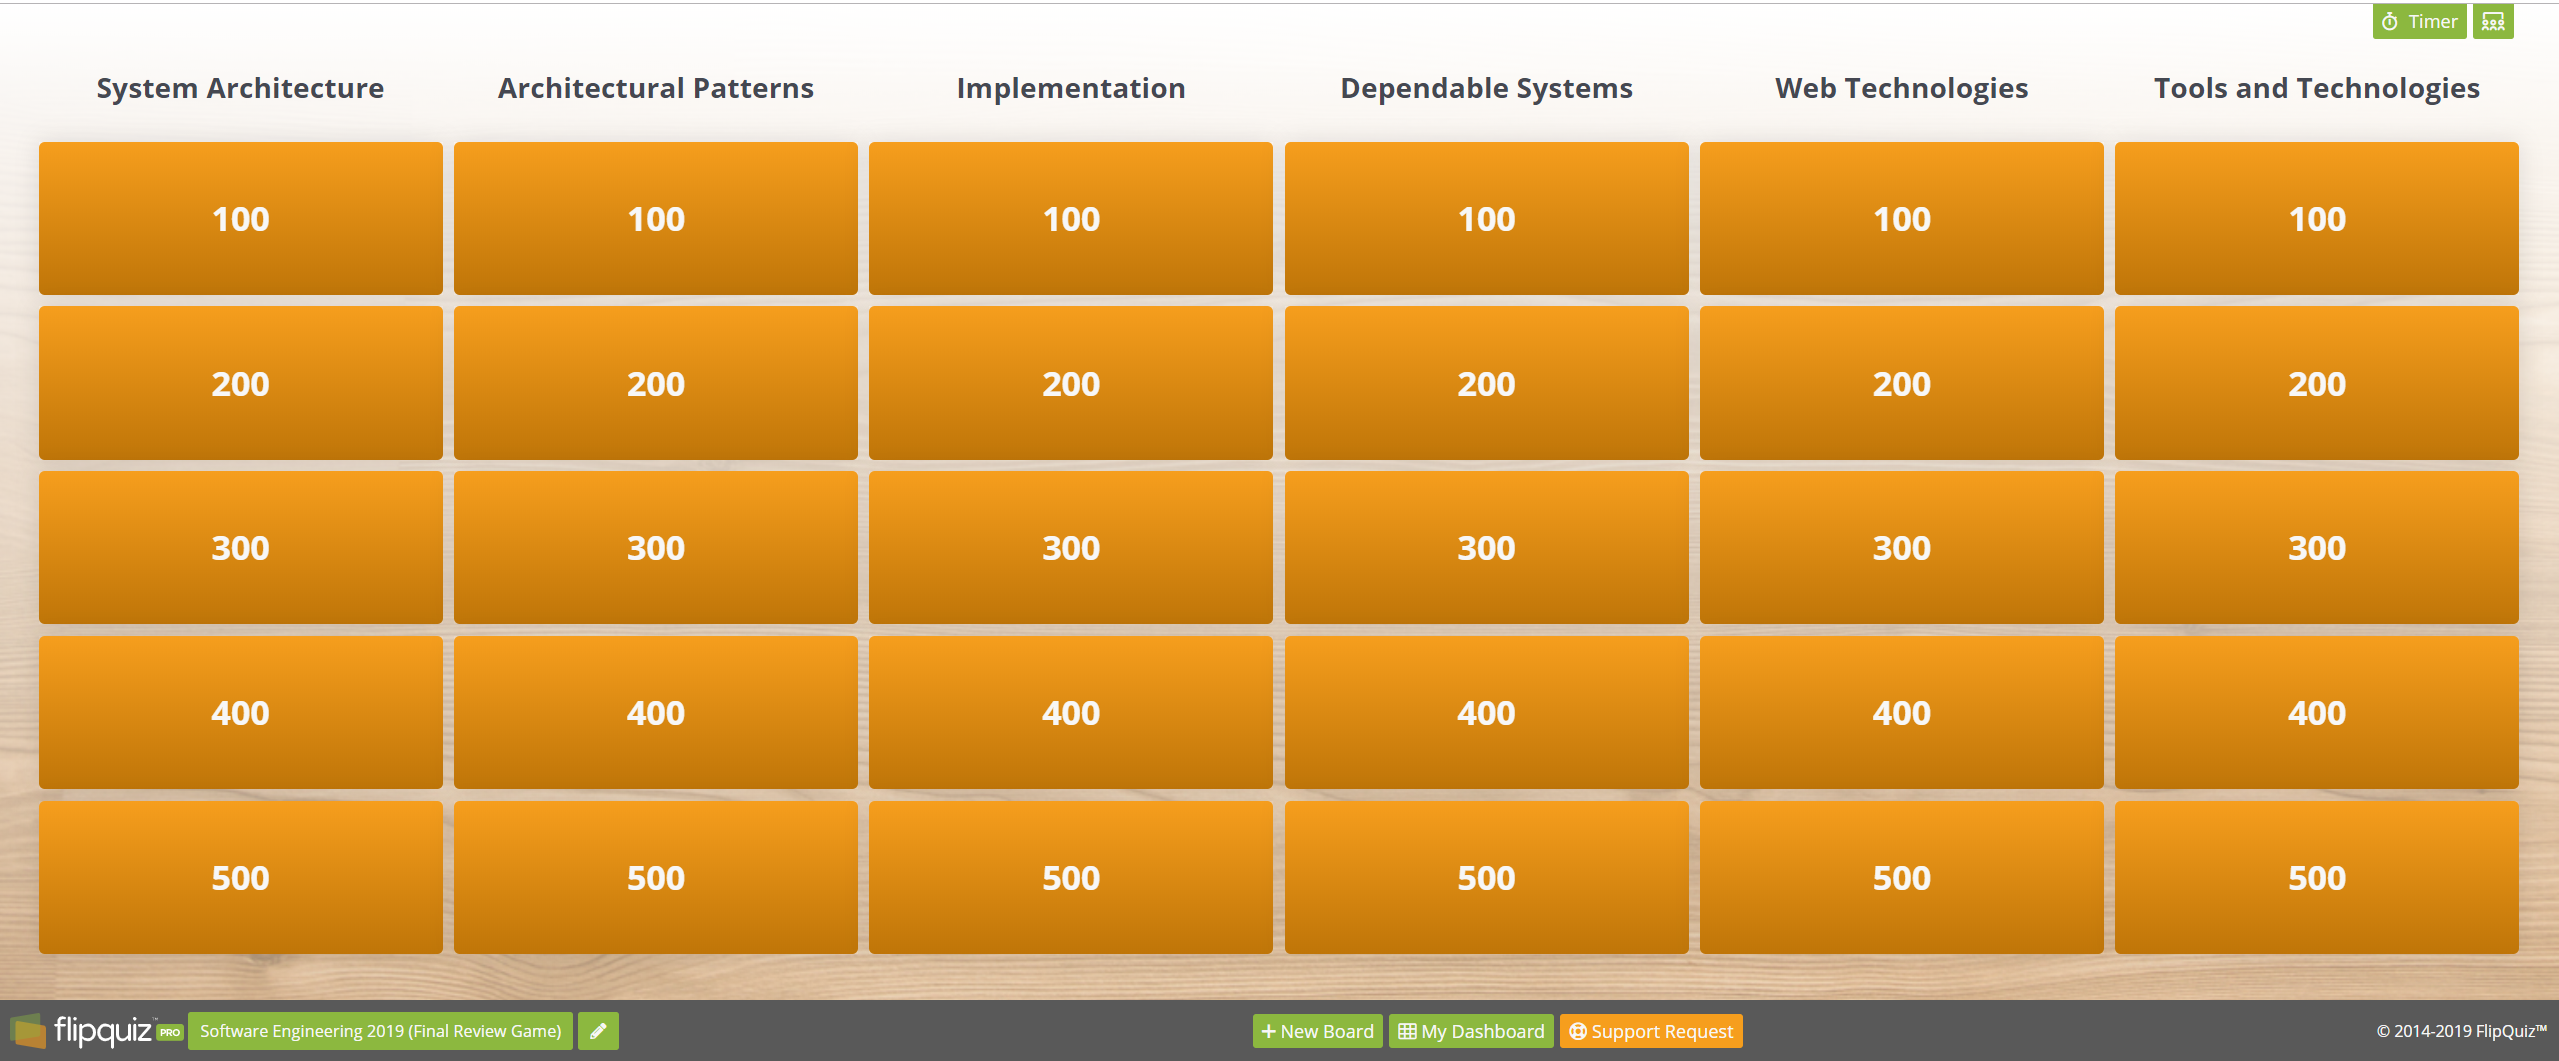
\includegraphics[width=.8\textwidth]{figures/FlipQuiz}
\caption{Jeopardy game in ECSE 321: Introduction to Software Engineering course}
\label{fig:jeopardy-ecse321}
\end{figure}

%\subsection{Student feedback}

%\subsection{Summary of teaching}




%\subsubsection{Final reflections}

%\paragraph{Course-specific reflections: ECSE 321}

%\paragraph{Course-specific reflections: ECSE 429}



\section{Talent Care and Student Supervision}

\subsection{Summary of past supervision activities before joining McGill University ( -2015)}


\paragraph{Supervising PhD and MSc theses.}
Starting from my early postdoctoral years, I have been very active in talent care by supervising MSc and PhD students. I have been the \emph{main scientific advisor of 4 PhD completed students} (István Ráth, Ákos Horváth, Gábor Bergmann and Ábel Ujhelyi) and co-supervised 3 more completed PhD students. I also supervised 20+ MSc theses since 2001. Four papers written with my PhD students as first authors received a best paper award at major international conferences of my field. Moreover, one PhD student was successfully competing at the STAF 2015 Doctoral Symposium winning the 1st prize. 


\paragraph{Supervising early research work.} 
23 scientific reports written by MSc students under my tutoring participated successfully in a national two-phase (faculty and national-level) \href{http://www.otdt.hu/hu/cms/otdk/orszagos-tudomanyos-diakkori-konferencia/}{Scientific Students’ Associations Conference} organized for students who carry out early research work in Hungary. Early research results achieved by MSc students provided a basis for over 25 scientific publications published at international conferences. In 2009, I was selected as a \href{http://www.otdt.hu/page/kituntetesek/mak2009.php}{Distinguished Tutor} by the National Scientific Students Council (OTDT), a national prize requiring 10 years of successful tutoring, awarded bi-annually to only 3 tutors in the field of computer science. This way, I started to focus on talent care very early, in fact, as a 1st year PhD student. I was the \emph{first ever recipient} of the \href{https://otdk2017.mik.uni-pannon.hu/index.php/eredmenyek}{Csanád Imreh Award}, commemorating the Hungarian researcher who died %tragically 
at a young age. 

\paragraph{Careers of former students.} Together with 4 of my former PhD students (István Ráth, Ákos Horváth, Gábor Bergmann and Ábel Hegedüs), we \emph{founded a start-up company, IncQuery Labs Ltd.} in 2013 to provide industrial exploitation of our research results and our expertise in model-driven engineering. András Balogh (whom I co-supervised) is now Chief Technology Officer at ThyssenKrupp Presta Hungary. Four of my former MSc students worked for Google, several of them went for \emph{large international companies} Nokia, Ericsson, Lufthansa Systems, National Instruments or small \emph{innovative startups}.


\subsection{Supervision activities (since 2016)}

\paragraph{Supervising PhD students}
In 2015, I simultaneously applied to the professor position at McGill University in Canada and to the prestigious 
\href{https://mta.hu/lendulet}{Lendület research chair position} funded by the Hungarian Academy of Sciences in Hungary. 
As I succeeded in both cases, I had the unique opportunity to lead a Trans-Atlantic research group and supervise 5 PhD 
students and co-supervise another 3 PhD students.  In addition, I also served as a scientific mentor of two young assistant 
professors at BME who were involved in the Lendület project.

Given that those PhD students were in different stages in their career and McGill's policy disallows a PhD student to start 
later, Márton Búr ended up restarting as a PhD student at McGill in Fall 2017. The other PhD students (namely, Gábor 
Szárnyas, Oszkár Semeráth, Csaba Debreceni, Ákos Hajdu, Vince Molnár, Kristóf Marussy) became graduate research 
trainees at McGill University for several months while continuing their PhD studies in Hungary (András Nagy gave up his PhD 
studies in Winter 2017 due to family reasons). All of these PhD students have been doing research along a research program 
related to model-based design and analysis of cyber-physical initiated by me (and co-funded both in Canada and Hungary). 

I have continuously been involved in the supervision of those students where I acted as the main supervisor (namely, 
Márton, Gábor, Oszkár and Csaba) on a weekly or sometimes on a daily basis when writing important publications. While 
Márton has been around me throughout the entire academic year when I had teaching duties, typically two PhD students 
visited me at a time (on a round-robin basis) as graduate research trainees between September and June. I supervised all the others who were not actually at McGill via 
teleconferencing. Those students I co-supervised (Ákos, Vince and Kristóf) visited me at McGill University as graduate 
research trainees once. During summer-time (July, August), I spent more time in Hungary where I could have in-person 
discussions with PhD students of the Lendület project (and did teleconferencing with Márton in the meanwhile). 

Detailed evidence of my successful supervision will be provided below, but most importantly, Oszkár and Gábor defended 
their PhD thesis in June 2019, Csaba's thesis is already under review and his public defense is expected in Fall 2019, while 
Ákos and Vince are PhD candidates (to defend within a year). Moreover, since Fall 2017, Márton Búr has been making 
substantial progress in his PhD studies at McGill University thus his research seminar is scheduled in September 2019.


\paragraph{Supervising MEng students}
Starting from Winter 2018 (and after severe delays caused by visa problems), I have been supervising MEng students at McGill University. By now, I have a very international and diverse group with of five MEng students, namely, Maruthi Rangappa (from India, started in W2018), Jasvir Kaur Dhaliwal (from India, started in W2018), Faizan Khan (from Pakistan, started in F2018), Aren Babikian (from Quebec, started in W2019), Sebastian Pilarski (from Canada, started in W2019). I collaborate them with weekly meetings and extra teleconferences when my students have some roadblocks. With Aren and Sebastian, I have started collaboration while they were still undergraduate students at McGill, and they have already committed to continue for the PhD studies.  

\paragraph{Supervising undergraduate students}
I have also been active in supervising undergraduate students at McGill University in two different ways.  Since 2017, I have been supervising a total of six projects as part of Summer Undergraduate Research in Engineering (SURE) program involving a total of 9 talented undergraduate students at McGill. One of those projects ended up with a joint publication where undergraduate students were co-authors. Furthermore, I have been supervising a total of 9 Design Projects involving a total of 29 undergraduate students. 

\subsection{Evidence of effective student supervision}

The effectiveness of my graduate supervision can be highlighted by numerous papers published at leading scientific 
conferences and journals of my field including international awards received by some of our papers or by my students 
themselves. 

\paragraph{Successful PhD defenses}
Since joining McGill University in 2016, three of my PhD students successfully completed their PhD defenses and a fourth student is a PhD candidate. 

\emph{Gábor Szárnyas} (my PhD student at BME, graduate research trainee at McGill) successfully defended his thesis on "Query, Analysis, and Benchmarking Techniques for Evolving Property Graphs of Software Systems" in June 2019. In the same month, \emph{Oszkár Semeráth} (my PhD student at BME, graduate research trainee at McGill) also defended successfully his PhD thesis on "Formal Validation and Model Generation for Domain-Specific Languages". Furthermore, \emph{Csaba Debreceni} has also submitted his PhD thesis on "Advanced Techniques and Tools for Secure Collaborative Modeling", which will be defended in Fall 2019. 
While Gábor, Oszkár and Csaba did not restart as McGill PhD students (as they were starting their 2nd/3rd year of PhD studies), but they regularly visited my as graduate research trainees. Since most of their supervision was carried out since I joined McGill University, I regard them as PhD students I graduated as a McGill professor. 

\emph{Zoltán Ujhelyi} (my PhD student at BME) also successfully defended his PhD thesis on "Program Analysis Techniques for Model Queries and Transformations" in 2017, but in his case, most of his scientific progress towards the PhD was made before I joined McGill University. Nevertheless, I still supervised him while writing his thesis as a McGill professor.  Finally, it is worth highlighting that \emph{Márton Búr} (my PhD student at McGill) will have his Research Seminar (ECSE703) in early September 2019, i.e. at the beginning of his 3rd year of PhD at McGill University, thus his progress towards his PhD is also very promising.

\paragraph{Papers co-authored with my graduate students}
Since joining McGill University in August 2016, I published four peer-reviewed journal papers (including 2 in Software and Systems Modeling and 1 in IEEE Software) co-authored with my PhD students,  and two more journal papers are accepted for publication. Five out of these six papers had my PhD students as first authors. 

In addition, we published 18 regular and tool demonstration papers and 2 more papers are accepted at leading scientific conferences of my research area (including 8 at MODELS, 2 at ICSE, 2 FASE, 1 at ESEC/FSE, 1 at ICMT) together with my graduate students. Out of these 20 papers,  14 papers had a student first author who I supervised or co-supervised. 
We also published 3 more peer-reviewed papers at co-located workshops of major conferences. 

\paragraph{Best/Distinguished paper awards}
Two papers having my PhD student as co-authors received prestigious paper awards at prestigious international conferences. 

The paper co-authored by Márton Búr (my PhD student at McGill), Gábor Szilágyi, András Vörös and myself on "Distributed Graph Queries for Runtime Monitoring of Cyber-Physical Systems" \cite{fase2018-cps} received the \emph{ETAPS EASST Best Paper Award} from the European Association of Software Science and Technology (\href{http://easst.aulp.co.uk/}{EASST}) at the 21st European Joint Conferences on Theory and Practice of Software (ETAPS), which is the primary European forum for academic and industrial researchers working on topics relating to Software Science. In this case, one paper was selected by the EASST committee out of more than 140 papers accepted at the six main conferences of ETAPS. As a follow-up of the award, we were invited to submit an extended version of our work to the Springer journal Software Tools on Technology Transfer which also paper \cite{sttt-2019} got accepted recently. 

The paper co-authored by Gábor Bergmann (formerly supervised at BME), Csaba Debreceni (my PhD student at BME, graduate research trainee at McGill), István Ráth and myself on "Query-based access control for secure collaborative modeling using bidirectional transformations" \cite{MODELS2016-access} received an \emph{ACM Distinguished Paper Award} at the IEEE / ACM 19th International Conference on Model Driven Engineering Languages and Systems (MODELS 2016). In this case, three papers were selected out of the total of 42 accepted regular papers. Again, we were invited to submit an extended version to a special issue in the Software and Systems Modeling journal (Springer), the top scientific journal of my direct research field, which was recently published \cite{sosym2017-mondo}.


\paragraph{International awards won by my graduate students}

My graduate students were also very successful at research contests organized for graduate students at major international conferences.  \emph{Gábor Szárnyas} (my PhD student at BME,  and graduate research trainee at McGill) won the 1st prize at the ACM Student Research Competition (SRC) at the MODELS 2016 conference, at the main forum of model-driven engineering. Furthermore, he also won 2nd prize at the ACM SRC contest organized at the SIGMOD 2018 (International Conference on Management of Data), which is a top conference in the field of databases. As a further success story, Gábor received an invitation to the program committee of the International Conference on Extending Database Technology (EDBT) right before his PhD defense, which shows the great level of research scientific independence he achieved (as databases are not my direct research area!). 

In addition, \emph{Csaba Debreceni} (my PhD student at BME,  and graduate research trainee at McGill) was also successful at the ACM Student Research Competition (SRC) at the MODELS 2017 conference winning the 1st prize. He also published follow-up papers in the IEEE Software and Software and Systems Modeling journals. 


\paragraph{Success in supervising of early research work}

I have successfully continued involving talented undergraduate students in research and persuading them to pursue 
graduate studies afterwards. Aren Babikian and Sebastian Pilarski, two of my current MEng students at McGill University 
started their research in the Summer Undergraduate Research in Engineering (SURE) program, and they became co-authors 
of a tool demonstration paper \cite{icse2019-tool} published at ICSE 2019 thanks to their contributions. 


%All of my \emph{seven best paper awards had one of my PhD students} as the first author. 

%prestigious international Student Research Contests and Doctoral Symposiums (2x 1st prize at MODELS, 1x 2nd prize at SIGMOD, 1x 1st prize at STAF conferences).

\section{Educational Leadership and Teaching Development}


\subsection{Educational leadership experience at BME}
%(on research group, department, faculty, national level) 
At BME, I was the \emph{operative leader} of the \href{http://inf.mit.bme.hu/en/}{Fault Tolerant Systems Research Group} (consisting of over 20-25 members) between 2012 and 2016. Within this role, I was in charge of coordinating many aspects of the everyday life and duties of the group including the strategic supervision of educational activities. 

Since 2012, I have been a member of the \emph{strategic executive board of the department}. In 2013, I was nominated as a \emph{department representative at faculty-level coordination meetings} aiming for the development of a new curriculum on the MSc level, which officially started in February 2015. I have continuously been serving in a \emph{cross-departmental committee for talent care} since 2006. 

On the faculty-level, I am member of the Informatics Doctoral School at the Faculty of Electric Engineering. Between 2014-16, I have been serving on the committee of the Doctoral School on Software Engineering (Informatics) to shape the education program of PhD students. On the national-level, I am a \emph{member of the Informatics Scientific Committee of the Hungarian Academy of Sciences} (elected as the youngest member first in 2011 and re-elected in 2014 and 2017). I was an external member of the Informatics Doctoral Committee of University of Szeged.

\subsection{Educational leadership experience at McGill University}

%At McGill University, I served on \emph{various senior committees on the department level} including faculty search, graduate student ranking for scholarships, strategic advisory board of the department chair, tenure and reappointment committee. On the university-level, I have been elected to serve as one of the two the \emph{representatives of Faculty of Engineering at the Council of Graduate and Postdoctoral Studies}. 

I also serve as the \emph{program director of the upcoming software engineering co-op program} (expected to start in 
Fall 2020) where undergraduate students will need to spend four compulsory internship terms at companies. In that role, I 
have been working on the key policies, guidelines, student and employer evaluation forms related to the co-op terms since 
Fall 2018 together with Ms. Lorraine Donald (Industry Liaison Associate at the Faculty of Engineering, and future chief 
program administrator for the software engineering co-op program). 

The program needs to be calibrated in a way that more than 500 undergraduate students would find internship-like 
placements at companies each year for a 3-4 month semester. To address the challenge related to such a high number of 
students, we have made significant investment in the future software-based automation of the key business processes of 
students going on co-op terms. As a key activity initiated by me was to develop a prototype system for handling co-op terms 
as the group project of the Winter 2019 edition of the ECSE321 Introduction to Software Engineering course. This initiative 
was a major success and several projects were demonstrated in front of several McGill employees who currently manage 
co-op programs. 

Furthermore, I have also been voluntarily acting in the pilot project run at McGill to install and host GitHub Enterprise on McGill premises (i.e. to have a private installation of the popular version control system ), and I provided valuable feedback to the working group during the Winter 2018 edition of the ECSE321 course.

\subsection{Teaching and Learning Training Received}
Since joining McGill University, I have been actively attending various training sessions related to teaching and supervision as summarized in the following list:

\begin{itemize}
\item \emph{Supervisory Alliance Training} organized by GPS (Graduate and Postdoctoral Studies)  2016 (2 hours)
\item \emph{Clarifying Expectations in Graduate Supervision} offered by GPS,  2016 (2 hours)
\item \emph{Mandatory Graduate Student Supervision Training} offered by the Faculty of Engineering,  2017 (2 hours)
\item \emph{How to write recommendation letters?} organized by GPS, 2017 (2 hours)
\item \emph{Equity Training} offered by the Faculty of Engineering, 2017 (2 hours)
\item \emph{Postdoctoral Fellows Financing} offered by GPS, 2017 (2 hours)
\item \emph{Course design workshop} offered by Teaching and Learning Services (TLS), 2018 (2 days)
\end{itemize}

%\section{Teaching and graduate supervision philosophy}
%
%Most of my courses have been organized along a common scheme. Students need to invest significant amount of work in completing a \emph{team project} of 3-5 persons. I assign a \emph{complex software/systems engineering challenge}, and ideally with a real customer, where students need to \emph{use modern software technologies} (e.g. IDEs, version control systems, etc.) and project management frameworks (like Basecamp, Trello) while learning also foundational concepts. 
%
%Maintaining the attention of students during lectures can be a challenging task. I try to postpone abstract mathematical definitions to the point when the main concepts are sufficiently demonstrated by small examples first. I frequently use various \emph{best practices of active learning} during my lectures (e.g. bug hunts on ill-formed software, various games and quizzes, small challenges discussed in small groups). I often \emph{demonstrate the practical relevance of concepts using real-world examples} and industrial case studies sometimes presented by industrial collaborators within invited lectures. Usually, \emph{my lectures are complemented with tutorials} on key technologies (e.g. Eclipse technologies or multi-tier web applications) actively co-developed by my graduate students which also provides a first teaching experience for them. 



%\begin{figure}
%\centering
%\includegraphics[width=.8\textwidth]{figures/teaching-eval}
%\caption{Teaching evaluation at McGill Univeristy}
%\label{fig:teaching-eval}
%\end{figure}

%%\appendix
\chapter{Course Evaluation Results for ECSE 321 (W18)}
\label{sec:course-eval-results}
\lfoot{Course Evaluation Results for ECSE 321 (W18)}
%\rfoot{Course Evaluation Results for ECSE 321 (W18)}

This appendix reproduces the complete set of comments from the ECSE 321 course which I received right after I initiated the modernization of software technologies used within the course. The course is a required course in the Software Engineering and Computer Engineering curriculum, as well as in the Software Engineering Minor selected by electrical engineers and mechanical engineers. As such, in each semester, the course receives some 75-100 students with a very different background, but with very little knowledge of software technologies of industrial relevance. While most of the students have completed one or two programming courses, this is the first time that they have to work on a real (complex) software engineering project. 


Below, I present the students' feedback separately for each question, and I highlight how the course feedback improved after I carried out the modernization of software technologies.

\small

\begin{table}[h]
\footnotesize
\begin{tabular}{@{}p{12cm}p{1.1cm}p{1.1cm}@{}}
\toprule
\textbf{Question} & \textbf{W17} & \textbf{W18} \\ \toprule
\textbf{Q1: Overall, this is an excellent course.} & \textbf{3.8} & \textbf{4.5} \\ %\midrule
\bottomrule
\end{tabular}
\end{table}

\begin{itemize}[leftmargin=0.5cm]
\item Great course, material is very representative of real life problems 
\item Provides a great overview of the software engineering practice. 
\item Even though it was a fully packed course, the amount of things we learned is amazing and I really enjoyed taking this class with Prof Varro 
\item Love the changes to this course, you actually learn about technologies that are being used in the industry currently which makes this course so valuable 
\item This course is definitely alot different than all my other courses that I have taken. It for sure had the steepest learning curve. My level of knowledge of software is so much higher now than when I started this semester. It really opened my eyes to my strengths and weaknesses in this field, and how much I really enjoy it. I loved the fact that it gave me a better sense of understanding of what I was getting into. Although the steep learning curve and the "learning by doing" them of this course is great, it sometimes had its downsides. It would seem sometimes a little chaotic, when we would just be handed something to do/deal with without getting remotely enough information on it ( eg: assignment 1, Jenkins, etc..). I understand that these in themselves were some of the best parts about the course (and the most I learned new things in), but the approach could have definitely been improved, maybe take things a tad slower for us. And, as Prof. Varro would say, nevertheless, I can say that this course gave me my favorite experience out of all my classes at McGill. Thank you! 
\item Learned lots of new things but every subject was gone over way too quickly. For someone who's minoring in software and majoring in electrical with no prior software experience, this class was a nightmare. Every subject was taught to us as if we already knew the subject material and every piece of jargon. 
\item This class in an awesome class. Maybe software tools that we will eventually use in our career thus nice to see them during school year. Adapts to new technologies thus improve with time to use software that are used out on the market 
\item Learned so much! 
\item Theory covered is good, but the scope of the work compared to what is taught feels disproportionate. The flow of the assignments and project felt odd as well. The entire first assignment was to implement a small application using a ton of new technologies, and we only learn about them/how to apply them/proper testing methods etc. after this assignment is due. While the assignment was great to have in terms of reference material, wasn't constructive to learning as much as the actual project was. 
\item This course made me develop a passion for programming (although I am an electrical engineering student). It has been the most interesting and educational course I have taken. So much effort is put in this course from the detailed Hands-On tutorial document, to the project requirements supported by ‘real’ clients, and finally, the interesting games! 
\item Varro really makes this class seem a lot easier than it really is, learned a great deal of useful topics and the main idea of software engineering. 
\end{itemize}

\begin{table}[h]
\footnotesize
\begin{tabular}{@{}p{12cm}p{1.1cm}p{1.1cm}@{}}
\toprule
\textbf{Question} & \textbf{W17} & \textbf{W18} \\ \toprule
\textbf{Q2: Overall, I learned a great deal from this course.} & \textbf{4.2} & \textbf{4.5} \\ %\midrule
\bottomrule
\end{tabular}
\end{table}

\begin{itemize}[leftmargin=0.5cm]
\item The most I've ever learned from a single course! 
\item Would like to add that a bit more time should be spent on learning Android rather than just the setup 
\item I learned in this course more than i learned in my 3 years at McGill! 
\item Gives enough details about the different activities that shape the software development process, as well as guidelines and patterns to follow. 
\item I learned more in terms of programing than software 
\item Did not have a strong base, and I feel like even though it is a lot for one course, it is great. 
\item Was challenging, but helped learn a lot. 
\item Learning how to create a web frontend and Android frontend and connecting them to the backend was very interesting and made for an enjoyable project. 
\item Feels like too much of the content from this course overlaps with ECSE 223. 
\item I learned over 3 new programming languages within 3 months, I was able to design a web and android applications. I had an idea of how programming is used in the real market. 
\item As other students have said, there is a great deal to learn in this course; however, by the same token, there may be too much to learn. 
\end{itemize}

\begin{table}[h]
\footnotesize
\begin{tabular}{@{}p{12cm}p{1.1cm}p{1.1cm}@{}}
\toprule
\textbf{Question} & \textbf{W17} & \textbf{W18} \\ \toprule
\textbf{Q3: Overall, this instructor is an excellent teacher.} & \textbf{4.3} & \textbf{4.4} \\ %\midrule
\bottomrule
\end{tabular}
\end{table}

\begin{itemize}[leftmargin=0.5cm]
\item Professor Varro is by far one of the most helpful, dedicated professors at McGill. I have never seen a professor go out of his way to this extent to help their students. His slides and assignments are there to make sure you've learned everything you need to learn. Hope to take my future classes with him too! 

\item Daniel Varro has been one of the best teachers I have had at McGill. He uses effective learning methods that force the student to truly understand the material. Professor Varro is a strong believer that students should not be spoonfed solutions and that self-learning is an invaluable skill. This course was therefore very refreshing in this sense and these teaching methods made me feel I was truly understanding the material which I found very fulfilling. Professor Varro is also quite industry-orientated and has adapted the course to match the current tools/languages currently being used in industry. I believe this is very important, particularly in computer/software where the skills and trades are shifting at fast paces. I would say Professor Varro is one of the few professors I have had at McGill who seems to truly care about his students and goes above and beyond to help them learn. Having said that, the professor was a little ambitious when it came to what he expected of the students. Many of us have a full course load as well as part-time jobs/ extra-curricular activities. Also as a Mechanical Engineering student my only previous knowledge was COMP208 so the learning curve was steep. This is a 3-credit course and it is hard to expect students to put 20hr+/week on deliverables. To help lessen this workload I would suggest that the project not include Android. Also the assignments, although relevant and helpful, could be taken out as the project is already substantial. Finally, for the final project deliverable I would suggest that it be less focused on documentation but more on functionality. We have spent a long time documenting all our processes and it is very tedious to have to document everything again when we are focused on completing the actual software! To conclude, Professor Varro has made this a fantastic and rewarding course. 
Starting with basic computational skills in C, Fortran and Matlab I now feel confident as a beginner Full-Stack engineer. 

\item Great professor, explains material clearly and succinctly. 

\item Amazing teacher! It's really amazing how much he's there for his student! It would be my honour to work with you some day! 

\item Cares about his students. Pushes and encourages excellence. Knowledgeable about the course. 

\item Can barely speak a word of English. Stutters nonstop and does thinks course material is completely useless. Meanwhile his slides are unreadable and completely incomprehensible when studying. 

\item Very intelligent man, very helpful and patient with his students. 

\item Extremely dedicated and knowledgeable prof 

\item Good person, interested in the success of his students, but lectures are a little boring... mid tone, classes are not so engaging... difficult too to make this type of content interesting when they are often things that we learn was we actually do work and work in teams.

\item He really cares that you learn the material while also challenging you 

\item The professors seems to be very passionate about the material which makes his classes very engaging. He encourages asking questions and makes sure we absorbed all the challenging material. He puts a lot of effort ensuring that we got all the help we needed for the project and the assignment. 

\item Very approachable prof, no bad comments 
\end{itemize}

\begin{table}[h]
\footnotesize
\begin{tabular}{@{}p{12cm}p{1.1cm}p{1.1cm}@{}}
\toprule
\textbf{Question} & \textbf{W17} & \textbf{W18} \\ \toprule
\textbf{Q4: Overall, I learned a great deal from this instructor.} & \textbf{4.2} & \textbf{4.3} \\ %\midrule
\bottomrule
\end{tabular}
\end{table}

\begin{itemize}[leftmargin=0.5cm]
\item One of my top 5 professors at McGill. 
\item Tutorials were very beneficial. 
\item Had to learn most of the material by myself 
\end{itemize}

\begin{table}[h]
\footnotesize
\begin{tabular}{@{}p{12cm}p{1.1cm}p{1.1cm}@{}}
\toprule
\textbf{Question} & \textbf{W17} & \textbf{W18} \\ \toprule
\textbf{Q5. The instructor was well organised in class and presented the material clearly.} & \textbf{4.1} & \textbf{4.2} \\ %\midrule
\bottomrule
\end{tabular}
\end{table}

\begin{itemize}[leftmargin=0.5cm]
\item It will be better if more detailed examples can be provided, especially for modeling part and integration and system testing.
\item Would be nice if the nice class material could more explicitly cover the project material as a side by side aid. 
\item Lecture slides are very informative and clear. The material covered was synchronous with the projects and the assignment. 
\item I think that the class slides were a little ambiguous when studying them for evaluation like project deliverables, assignments, and the final exam. 
\end{itemize}

\begin{table}[h]
\footnotesize
\begin{tabular}{@{}p{12cm}p{1.1cm}p{1.1cm}@{}}
\toprule
\textbf{Question} & \textbf{W17} & \textbf{W18} \\ \toprule
\textbf{Q6. The instructor used effective teaching methods.} & \textbf{4.2} & \textbf{4.2} \\ %\midrule
\bottomrule
\end{tabular}
\end{table}

\begin{itemize}[leftmargin=0.5cm]
\item He encouraged participation during the class, which made us understand and absorb the material better. He used revision games to make the material entertaining. He offered bonus marks for outstanding performance, which was very motivational! 

\item Would be very helpful if more examples/questions on class material were provided to learn as we progress. 

\item I like the inclusion of group activities; other times, I find the class a little dry. 

\item Slides are not strong slides. Even with them, there is no chance in succeeding this class. Must listen to what he says. Thus, I believe that for future classes, it would be best if he gave the lecture slides before class, because even though they are given, they are not a lot of information on it, or at least precise since most of it thought by Varro verbally. Thus, I still believe that people will attend class and it is easier to take notes as he goes since not a lot of words are provided on the slides. 

\item The slides were not incredibly helpful or detailed. A great majority of things I learned from this class was during the project, which I do not think is a good thing. However, it would have been good to learn more from the lectures. 

\item I believe that professor Varro should first clearly present what he is talking about and how and why it works then go into the code. As a student, I was very confused what he was talking about. Assumes we know too much. 

\item More examples of diagrams please! 

\item The slides are good while in class (lecture accompanies by many visuals) but it is hard to study them outside of class due to lack of context/text in a lot of slides. 
\end{itemize}

\begin{table}[h]
\footnotesize
\begin{tabular}{@{}p{12cm}p{1.1cm}p{1.1cm}@{}}
\toprule
\textbf{Question} & \textbf{W17} & \textbf{W18} \\ \toprule
\textbf{Q7. The instructor was responsive to students’ questions and concerns, given the class size.} & \textbf{4.5} & \textbf{4.7} \\ %\midrule
\bottomrule
\end{tabular}
\end{table}

\begin{itemize}[leftmargin=0.5cm]
\item The professor is very supportive and answers all our questions. He stays answering the students after each lecture, during the office hours, through emails and on myCourses discussion board where there's more than 200 posts. Most of the students are form other majors (taking a minor in Software), and they took at most 2 programming courses. So, they asked a lot of questions and required a lot of help. The professor and the TAs were always there for us. And the result: by the end of the year, all groups have created a complicated well designed web page and Android app!! 
\item Always available to help students. Never seen a professor go out of his way to this extent to answer all emails, myCourses discussion board questions within minutes. 
\item Very responsive and very helpful. He replies to emails and questions within minutes! 
\item One of his better qualities. 
\item Always responds to emails and helpful in office hours 
\item E-mails were almost instantaneous in response. Feedback is detailed. Available after class and office hours every week for questions/concerns. 
\item He had one office hour during my class hours and it was very busy. 
\item Gives office hours. However the concept of it, of being like a conference is not so helpful I believe because its often really long before someone with a precise question gets answered. 
\item Always responded right away! thank you!! 
\end{itemize}

\begin{table}[h]
\footnotesize
\begin{tabular}{@{}p{12cm}p{1.1cm}p{1.1cm}@{}}
\toprule
\textbf{Question} & \textbf{W17} & \textbf{W18} \\ \toprule
\textbf{Q8. The instructor fostered an environment of mutual respect and engagement in learning.} & \textbf{4.7} & \textbf{4.8} \\ %\midrule
\bottomrule
\end{tabular}
\end{table}

\begin{itemize}[leftmargin=0.5cm]
\item Yes indeed! Did not feel stupid to ask questions. Varro was very receptive to all questions. 
\item Use of clickers helps keep students engaged, even if they don't know the answers. 
\item The class is very diverse in terms of majors (since it's a minor course), so the professor assigned the first assignment in groups to ensure that we involve with other students. He also encouraged asking questions and provided us with resources to learn on our own. 
\end{itemize}

\begin{table}[h]
\footnotesize
\begin{tabular}{@{}p{12cm}p{1.1cm}p{1.1cm}@{}}
\toprule
\textbf{Question} & \textbf{W17} & \textbf{W18} \\ \toprule
\textbf{Q9. The course materials contributed to learning the subject matter.} & \textbf{4.2} & \textbf{4.5} \\ %\midrule
\bottomrule
\end{tabular}
\end{table}

\begin{itemize}[leftmargin=0.5cm]
\item The first tutorial (Hands-On tutorial) was the most sufficient resource that we used throughout the final project. It was very detailed with screenshots and steps, as well as sources of error. It was very easy to follow especially with the buttons of the sections on the right. 
\item The project was very in-line with the course content. 
\item Had to learn a significant amount during office hours and by myself. 
\item Using a virtual machine was a terrible idea. I wasted many hours on this as it was extremely slow and it made completing the first assignment really really reslly much more complicated than it had to 
\end{itemize}

\begin{table}[h]
\footnotesize
\begin{tabular}{@{}p{12cm}p{1.1cm}p{1.1cm}@{}}
\toprule
\textbf{Question} & \textbf{W17} & \textbf{W18} \\ \toprule
\textbf{Q10. The course activities (inside and outside the classroom) engaged me actively in my learning process.} & \textbf{4.4} & \textbf{4.6} \\ %\midrule
\bottomrule
\end{tabular}
\end{table}

\begin{itemize}[leftmargin=0.5cm]
\item The revision games provided with the classes were not only educational and engaging, but also helped form groups and involve with the class. Also, the examples given in the lecture were very helpful in understanding the material. Finally, the design of the assignment questions! Most teams divide the work for the project, so some members have experience in software while others are responsible for documentation. However, the assignment help ensure that each student has experience with the important software topics of this course. They were very helpful and the feedback on each assignment was very detailed. 

\item I am really happy that Varro updated the project of this course to reflect newer frameworks and marketable skills. It gives us, the students, a taste of many of the qualifications asked for in internship applications, such as popular frameworks, testing, automation, and development techniques. 


\item The project deliverables were very fun to work on and encouraged me to learn quite a bit of additional information. 

\item The deliverables and assignments taught me a lot. However i must admit this course was a lot of work: I think having deliverables and assignments is a lot, the deliverables take a lot of time! 

\item Too much I don't like engagement 

\item Have to go look for everything myself online. Course activities and assignments are meant to reflect things learned in the class. It's kind of hard to do that when everything is impossible to understand 

\item Building the app was probably the most enlightening activity I did in university. Learned a lot. The small assignments however were a waste of time. I would strongly sugest you get rid of the Virtual Machine next year. Gives us double the trouble. To figure out the new software plus the VM. You used it to make easier for you to help us but since 99\% of the time we are on our own you should not apply this idea.

\item Great Assignments to keep with the lectures, and the project help us learn a lot. 

\item The group project teaches you so much! 

\item Yeah!! Impossible to do the project without learning!! 

\item Being the first class to have new technologies tested on makes it more difficult to feel like we're actively learning but rather just struggling to figure out the new system being implemented. That being said, the professor and TAs operated very well with their new technologies and helped as much as possible. 

\item I think the mentors that we had this semester should try and reach out to groups that they are assigned too, I know that they may be busy undergrads just like us but similar to how ECSE 211 have their TAs set up meetings for their groups (I know that the TAs in 211 don't have nearly as many groups), but I think it would be an idea to look into if possible 

\end{itemize}

\begin{table}[h]
\footnotesize
\begin{tabular}{@{}p{12cm}p{1.1cm}p{1.1cm}@{}}
\toprule
\textbf{Question} & \textbf{W17} & \textbf{W18} \\ \toprule
\textbf{Q11. The evaluation methods used in this course were fair and appropriate.} & \textbf{4.2} & \textbf{4.3} \\ %\midrule
\bottomrule
\end{tabular}
\end{table}

\begin{itemize}[leftmargin=0.5cm]
\item Grading scheme is fair. However, assignments and projects do not directly reflect the actual effort and understanding of students since they can use outside help for instance. There should be a more standardized evaluation such as a midterm. 

\item Group projects are terrible for people who are more competent than the average group member. You either have to do all the work to achieve your potential, or settle for a lower mark. 

\item None of the grading schemes were very descriptive in what they required. Got marks taken off because assignment instructions are way too vague. Project was supposed to be freeform but got many marks taken away for sections that involved more liberty. 

\item Varro was very fair with his expectations. 

\item I believe that the final exam was extremely difficult to complete because of how long it was. That is, I spent all three hours writing as fast as possible to ensure that I finished it. I also think that it was not extremely fair to have half of the exam be things from the lecture slides that we wrote on our crib sheet (this was just copying things from out crib sheet into our exam and didn't serve much purpose), and the other have of the exam require us to draw every possible diagram that we had seen, as making diagrams takes time and effort, and being rushed does not help us completing them. 

\item The one thing that irks me is the detail of some questions asked in this final as well as in-class ECSE 223 wherein some questions of vocabulary seem just pedantic, and by asking them while allowing open-book, these parts of the exam just become a test to see which student printed out the entire set of lecture notes to bring over the course of the semester for the sake of such a question. 
\end{itemize}

\begin{table}[h]
\footnotesize
\begin{tabular}{@{}p{12cm}p{1.1cm}p{1.1cm}@{}}
\toprule
\textbf{Question} & \textbf{W17} & \textbf{W18} \\ \toprule
\textbf{Q12. I was provided with useful feedback on my progress in the course.} & \textbf{3.8} & \textbf{4.4} \\ %\midrule
\bottomrule
\end{tabular}
\end{table}

\begin{itemize}[leftmargin=0.5cm]
\item Since the project was cumulative, meaning that each deliverable depends on the previous one, it was very crucial to have clear feedback. Feedback was very fast on assignments, projects and the final exam. It was very detailed so we used it as a resource for later deliverable. And finally, the idea of bonuses was very motivational! 
\item Every single assignment was graded with very detailed feed-back so I knew what was correct, and what to improve. 
\item Really detailed correction. we know exactly where we made our mistakes, and if needed TAs are present to go over with us for more understanding. 
\item Very good feedback! 
\item Comments given on assignments are not useful at all. 
\item Feedback on one deliverable would often come after the next was already due, making it harder to identify and address issues as they appeared. 
\item The feedback was quick 
\item Feedback on assignments and deliverables, aswell as time spent in office hours, were very beneficial for my understanding on the course material. 
\item Varro was a speedy marker! Marked exams in 1 day!!!!!!!!! 
\end{itemize}

\begin{table}[h]
\footnotesize
\begin{tabular}{@{}p{12cm}p{1.1cm}p{1.1cm}@{}}
\toprule
\textbf{Question} & \textbf{W17} & \textbf{W18} \\ \toprule
\textbf{Q13. The course workload was appropriate, given the credit weight and the scheduled activity hours.} & \textbf{3.5} & \textbf{3.5} \\ %\midrule
\bottomrule
\end{tabular}
\end{table}

\begin{itemize}[leftmargin=0.5cm]
\item It is a lot of work, but you do learn a lot 
\item The workload is a bit too much in terms of the hours needed to achieve the deliverable, but nonetheless I can't see how else we could learn from this course. You learn so much in this course, in the most interactive, engaging way. The project is so useful, and fundamental to this course. 
\item Workload for team project is large but can learn a lot from the project. 
\item Should be a 4 credit course with this amount of work. People are only just starting to learn This material and we can't be expected to be masters of it within a week. 
\item I really loved this course but I really think it's a lot of work, especially since most of us are taking 5 classes! 
\item Time spent on the project does not reflect the credit weight. Recommend to make the class 4 credits worth. 
\item I spend half my week working on this cources and the over half on my over 5 cources. Defently get rid of most of the assigments. 
\item We as a team have put way more hours into this class compared to others... could be a 4 credit class would be more appropriate considering all the new tools that one may not have learn before. The class was very overwhelming at first. But I guess it depends on the strength of people in programming thus a 3 credit class can also be appropriate. 
\item The project was very big, and took up a lot of time. I still think it was worth it though. 
\item Spent an incredible amount of time on this course(30+hours a week outside of class time), which is way more than the expected time I'd expect from a 3 credit course. Nevertheless, it was enjoyable. 
\item SO many hours of my life all weekends and evenings were dedicated to this course. The course SHOULD be worth 4 credits at least. Nevertheless I did enjoy the material. 
\item Scope of the project felt quite large given the time constraint and that many of the students in the class were taking ECSE 223 in parallel (and thus developing another application in their "down" time). 
\item This course should be a 4 credit course. 
\item I dont think the weight of each class component was fair in regards to the worklaod that came with each. The course project should be worth way way more as we spend the entire semester on it and for me even 40 hours a week on it. I didnt find it fair the final was worth so much and it was wayy too long of a final too. I couldnt even finish it. I think making it easier and worth less would be great. Also , I found assignments unnecessary. 
\item In teams where some individuals are not as experienced, the workload becomes heavily skewed. 
\end{itemize}

\begin{table}[h]
\footnotesize
\begin{tabular}{@{}p{12cm}p{1.1cm}p{1.1cm}@{}}
\toprule
\textbf{Question} & \textbf{W17} & \textbf{W18} \\ \toprule
\textbf{Q14. The course workload was appropriate, given the credit weight and the scheduled activity hours.} & \textbf{3.5} & \textbf{3.5} \\ %\midrule
\bottomrule
\end{tabular}
\end{table}

\begin{itemize}[leftmargin=0.5cm]
\item This is by far the most relevant class for software engineering. Information learnt is practical and the patterns and technologies learnt in this class can be used in virtually every software project. 
\item I LOVE SOFTWARE ENGINEERING IT'S SO MUCH FUN. 
\item The first time I understood the significance of each and every word in the slide, because we were constantly applying it every day to tackle the projects and assignments. 
\item Documentation is boring 
\item Yeah appreciate the work software engineers do! Am glad to be in Computer engineering though, more high level. 
\item This course was very interesting and engaging. Therefore, I developed a passion for programming which made me decide to apply for a minor in Software engineering. 
\end{itemize}

\normalfont



\end{document}

\chapter{Research Portfolio}
\label{sec:research-portfolio}
\lfoot{Research Portfolio} 
%\rfoot{Research Portfolio} 

%\begin{tcolorbox}[title=Summary of Excellence]
%My research primarily focuses on providing \emph{precise and scalable techniques} and \emph{software tools} used for engineering critical software-intensive systems with a recent focus on \emph{smart and safe cyber-physical systems} (CPS) deployed over decentralized, heterogeneous platforms. As the leader of an excellent research team with 15 PhD and 25+ Masters students I supervised or co-supervised, we received \emph{7x Best/Distinguished Paper Awards} at major peer-reviewed conferences of software engineering (3 of which since joining McGill). I also received \emph{two 10-year most influential papers} for past results achieved in my early career. My research papers received over 6700 citations yielding an h-index of 43. In the past 5 years, I was invited to deliver 6 keynote talks at international or national conferences or workshops, 10 talks at advanced schools, and 15+ talks at industrial events.
%
%\vspace{3pt}
%
%%\paragraph{A paragraph}
%Moreover, I have actively contributed to turn \emph{novel research results and prototype tools} first into \emph{industrial strength open source frameworks} then \emph{to innovative services and products} maintained by IncQuery Labs, a successful Hungarian company co-founded with my former graduate students and used by major international companies.
%% operating in the CPS domain.
%\end{tcolorbox}

\paragraph{Organization of research portfolio}

My career as an indepenent researcher consists two main stages. \textbf{Stage 1} is from 2004 when I started to independently supervise students at BME, which included 5 PhD students and numerous MSc students until 2014.
I successfully received a tenured position in 2009 and I was promoted to a full professor at BME in 2014, which I consider to be the end of this first stage. During these years, my research was primarily focusing on various model query and transformation techniques used in the model-based software and systems engineering for safety-critical systems. 

\textbf{Stage 2} (starting in 2015) has been carried out in a rather unique research environment.  I successfully applied to a professor position at the Department of Electrical and Computer Engineering at McGill University, and I also acquired a Hungarian prestigious and highly selective Research Chair position funded by the Hungarian Academy of Sciences to found the \href{https://mta.hu/lendulet/az-mta-lendulet-kutatocsoport-halozata-105402}{MTA-BME Lendület Cyber-Physical Systems Research Group} by \emph{initiating a new research program on designing and analyzing cyber-physical systems}. Since I got permission from my department to simultaneously pursue this research program both in Canada and Hungary, I was the \emph{scientific leader of a broad international research program} since 2015.
Altogether, I was main supervisor of five PhD students, but I also provided co-supervision or strategic guidance for five other PhD students and two junior faculty members at the Department of Measurement and Information Systems. I coordinated this Trans-Atlantic research group by teleconferences and by frequent visits of Hungarian students as McGill graduate research trainees.

% which involved 2 junior staff members (at BME), 10 PhD students (5 as main supervisor, 5 as co-supervisor or strategic ) and numerous masters and undergraduate students. 
%This research has been carried out in a rather unique and unconventional research environment. In 2015, I successfully acquired a Hungarian prestigious and highly selective Research Chair position funded by the Hungarian Academy of Sciences to run the \href{https://mta.hu/lendulet/az-mta-lendulet-kutatocsoport-halozata-105402}{MTA-BME Lendület Cyber-Physical Systems Research Group}. Here I was main supervisor of five PhD students, but I also provided co-supervision or strategic guidance for six other PhD students (partially affiliated to the project) who are supervised by young faculty members at the Department of Measurement and Information Systems. In response to the increasing direct political influence on academic institutes and research funding imposed by the Orbán Government in Hungary, I joined the Department of Electrical and Computer Engineering at McGill University as a full professor in 2016. Since then, I have been coordinating research of a virtual (trans-Atlantic) group with frequent visits of Hungarian students at McGill.


Therefore, the research portfolio of my tenure dossier is organized correspondingly to these two stages. First, I summarize 
my five most significant research contributions in Stage 1 (i.e. up to 2014-15), and then I provide in-depth details about my research in Stage 2 (from summer of 2015). Please note that my actual starting time at McGill University was delayed until the summer of 2016 due to work permit issues, but my NSERC Discovery Grant application was already submitted in 2015, thus this is the most logical presentation of my research activities in my opinion. 

%In this research statement, I first summarize the five most significant research contributions between 2000 and 2015, i.e. the time which already had impact, then I summarize recent lines of research from the last 5-6 years. Then, I will overview ongoing and prospective future lines of research. Finally, I present a summary of impact for three research papers written in different stages of my career.

\section{Past Research Contributions: Stage 1 (2004-2015)}

\subsection{Context}

In the past decade, model-based systems engineering (MBSE) has become a key technique for designing critical systems in application domains like avionics or automotive.%\cite{Broy2012,Whittle2014}. 
MBSE facilitates the systematic use of models on various levels of abstraction from an early phase of the development process in order to simultaneously \emph{increase productivity and quality} while \emph{reducing development costs} by avoiding costly re-design cycles compared to detecting the same problem by traditional testing. 

%System requirements and initial design 
System design is captured by \emph{high-level engineering models} using modeling languages (like UML, SysML, AADL, Capella). These models enable to immediately check design rules and well-formedness constraints imposed by the underlying platform (such as AUTOSAR or ARINC653) to design flaws early. Early \emph{hidden formal analysis of system models} can be carried out by generating various mathematical models by automated model transformations (MTs) to detect and eliminate conceptual flaws and quality bottlenecks. Results of precise mathematical analysis are back-annotated to system models, thus systems engineers can observe and correct these problems using a formalism familiar to them. 

%\begin{figure}[htb]
%\centering
%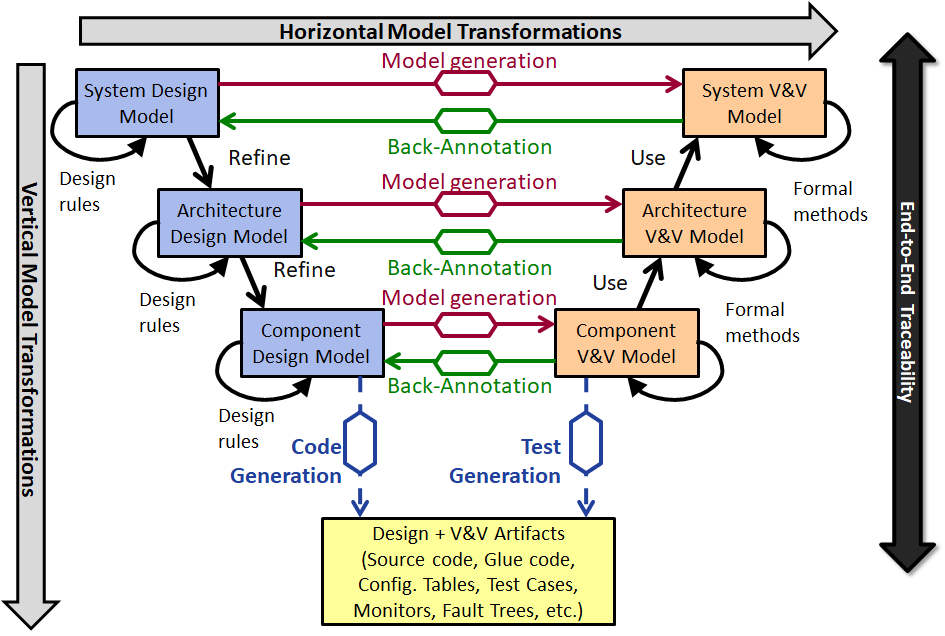
\includegraphics[width=.65\textwidth]{figures/mbse}
%\caption{Models transformations in model-based systems engineering}
%\label{fig:mbse}
%\end{figure}


Automated code generators (also called vertical MTs) improve productivity by synthesizing provenly correct source code of a safety-critical application from a validated model.% \cite{Sturmer-TSE2007}. 
In addition to source code generation, MBSE tools can synthesize other design artifacts (such as configuration tables, fault trees, test cases, documentation) and provide support for end-to-end traceability.% \cite{Aizenbud-IBMSystems-2006}. 
MBSE changes the traditional V-model of systems engineering into a Y-model where certain certification artifacts are synthesized automatically from models of proven quality used at different levels of abstraction.

%\subsection{Summary}
In Stage 1, my research was characterized by (1) proposing novel, foundational concepts, (2) developing innovative and scalable techniques, (3) architecting and maintaining cutting edge prototype tools based on solid foundations, (4) continuously benchmarking and empirically evaluating these tools, and (5) using these results at design time in a wide range of applications in tools used for engineering critical systems (like avionics and automotive). 

\subsection{Scalable incremental model queries: Techniques and tools}

\paragraph{Results.}
With my graduate students, G. Bergmann, M. Búr, Á. Hegedüs, Á. Horváth, G. Szárnyas, and I. Ráth, we developed highly scalable incremental techniques for continuously evaluating graph queries over large domain-specific instance models used in design and validation tools of critical systems. We turned scientific results \cite{models-2010-incquery,scp2015,models2014-iqd,icgt2015,sosym2016-viatra-invited} into mature scalable software tools, which instantly re-evaluate validation rules over domain-specific graph models with millions of elements. 

\paragraph{Impact.}
The \href{https://www.eclipse.org/viatra/}{VIATRA open source project} has been actively \emph{used at large companies and research institutes} (e.g. Thales, Airbus, Ericsson, ThyssenKruppPresta, Embraer, NASA JPL), and in \emph{industrial modeling tools} (e.g. Papyrus, Capella, Artop). It provides the basis of \emph{innovative products} (\href{https://incquerylabs.com/incquery/}{IncQuery for MagicDraw, IncQuery Server}) developed at IncQuery Labs Ltd. It has been \emph{regularly used a baseline in performance comparisons} by leading researchers (e.g. D. Kolovos, J. Cabot, H. Giese). I \emph{delivered several keynote talks} on related topics at major scientific conferences and summer schools. Related papers \cite{models-2010-incquery,icmt2011,ase2011-tool,ecmfa2011,models2014-iqd,scp2015,icgt2015,sosym2016-viatra-invited} have been cited over 400 times. 
% and \cite{models2018-tool} received a \textbf{Best Tool Paper Award} at the MoDELS 2018 conference. 

\paragraph{My role.}
All major contributors of the incremental graph query technology are my former PhD students. I have been the strategic leader of the research line until 2016 when the development of the open source framework was taken over by software engineers at IncQuery Labs Ltd, a high-tech company co-founded together with my former graduate students. This line of research has been funded by numerous national and international competitive research projects: I was the site leader at BME of \emph{collaborative European projects} (e.g. SENSORIA, SecureChange), and the principal investigator (PI) of an ERC Starting Grant application (CERTIMOT) which went to the final round, but became out of budget, and later it received partial funding from the Hungarian Research Agency (ERC-HU). 
%VIATRA technology received significant extra funding at IncQuery Labs, which is not detailed here. 


\subsection{Novel model transformations concepts}

\paragraph{Results.}
With my students, A. Balogh, Z. Balogh, G. Bergmann, Á. Hegedüs, Á. Horváth, I. Ráth, Z. Ujhelyi, we proposed novel model transformation concepts to capture mappings within and between various modeling languages. The scientific results provided foundations of the open source \href{https://www.eclipse.org/viatra/}{VIATRA} model transformation framework \cite{SCP2002,ASE2002,uml2004-meta,scp-2007,sosym2016-viatra-invited} which has been successfully developed along three generations since 2000. Novel concepts proposed by us for the first time include \emph{change-driven transformations} \cite{Rath-models09,sosym2011-cdt}, \emph{model transformation by example} (MTBE) \cite{models2006-varro,sosym2008-mtbe}, \emph{reactive transformations} \cite{icmt08-rbov08,icmt2015,sosym2016-viatra-invited} or \emph{model transformation slicing} \cite{ase2011-mtslice,icst2012}.

\paragraph{Impact.} 
In addition to its industrial use, we published our results on the VIATRA framework at major scientific venues of model-driven engineering including \cite{SCP2002,ASE2002,uml2004-meta,models2006-varro,scp-2007,Bergmann-icmt09,Rath-sosym09,Rath-models09,Bergmann-sttt10}, which have been cited well over 2000 times. The paper \cite{uml2004-meta} got the \textbf{10-year Most Influential Paper Award} at the IEEE/ACM MODELS 2014 conference (the main scientific forum of my research area), and I was invited to write an expert panel paper to the Software and Systems Modeling journal (SoSyM) \cite{sosym2016-viatra-invited}. Our first paper on change-driven transformations \cite{Rath-models09} received \textbf{Springer Best Paper Award} at IEEE/ACM MODELS 2009. The concepts of MTBE have been followed by 12 independent research groups worldwide. I delivered \emph{several keynote talks} at international conferences and summer schools on related topics.

\paragraph{My role.} 
The first open source version of VIATRA was developed by my graduate students, and I served as the strategic leader of the project until 2016 when development was taken over by IncQuery Labs Ltd. Therefore, I played key role in maturing a research prototype into an industrial framework. I was the main contributor (and hence, the first author) of the expert panel paper invited to the SoSyM journal.  I was the main supervisor of 5 PhD students and co-supervisor of 2 PhD students in addition to 20+ MSc students doing research and development on related topics. Co-founding IncQuery Labs enabled to keep together the core team for 15 years by now. I was the principal investigator (PI) of three IBM Faculty Awards, and an ERC-HU Starting Grant application and the site leader of various collaborative European projects (e.g. SENSORIA, SecureChange, MONDO) .

%My role in the related projects that funded this line of research is the same as in the previous line

\subsection{Performance benchmarks for model queries and transformations}
\paragraph{Results.}
Together with G. Varró and A. Schürr, we proposed the \emph{first performance benchmark for model transformation tools} in \cite{vlhcc05-vsv}. Since then, developing and maintaining performance benchmarks have been a focal topic of my research group. With my students, G. Bergmann, Á. Horváth, B. Izsó, G. Szárnyas, I. Ráth, Z. Ujhelyi, we systematically assessed the performance of various model query technologies \cite{Bergmann-sttt10,scp2015,ttc2015} of different modeling tools. 
%for different technological platforms along the Train Benchmark. 
In collaboration with researchers from University of Szeged, IncQuery was successfully used for detecting anti-patterns in source code of large projects \cite{csmr2014,ist2015}.

\paragraph{Impact.} 
Our first paper \cite{vlhcc05-vsv} triggered a series of annual Transformation Tool Contests (over 12 editions) and it received a \textbf{Most Influential Paper Award} at IEEE VL/HCC 2016. Moreover, \cite{csmr2014} received the \textbf{Best Paper Award} at CSMR-WCRE 2014. The Train Benchmark \cite{ttc2015} has been used by other researchers (e.g. D. Kolovos, X. De Carlos, G. Varró, G. Hinkel, H. Giese) for performance comparison from several independent research groups. Related papers have been cited over 275 times.

\paragraph{My role.} 
I was one of the three researchers who proposed the first benchmark for model transformations in 2005. 
%Benchmarking was a focal topic of my PhD student G. Szárnyas, while 
Later, I was a co-organizer of the first open transformation tool comparison as part of the AGTIVE 2007 conference \cite{agtive07-toolcontest}. My students (G. Bergmann, Á. Hegedüs, Á. Horváth, B. Izsó, I. Ráth, Z. Ujhelyi) made significant contributions to past benchmarking activities. I was the site leader at BME of the MONDO FP7 project, 
%and a collaborator in the MOGENTES FP7 project, 
which financed some of the related research activities.

\subsection{Rule-based guided design space exploration}

\paragraph{Results.}
Design space exploration (DSE) aims to derive design candidates fulfilling various design constraints from an initial design sketch by applying a pre-defined set of operations. We proposed the concept of \emph{rule-based guided design space exploration} \cite{Horvath-models09,sosym2011-csp,ase2011-dse,ause2015,ase2014,mpm2014} to incorporate complex structural consistency constraints frequently present in architecture models of automotive and avionics applications. The exploration process can be heuristically guided by hints obtained from the designer. DSE was applied to provide quick fixes in design environments built for business modeling \cite{vlhcc2011}. 

\paragraph{Impact.} 
Our paper \cite{ase2011-dse} at the IEEE ASE 2011 conference received an \textbf{ACM Distinguished Paper Award}. Other researchers (e.g. H. Vangheluwe, S. Zschaler and M. Wimmer) conducted research building on our results. Key papers \cite{Horvath-models09,vlhcc2011,sosym2011-csp,ase2011-dse,ause2015,ase2014} received over 150 citations in total. 
%The VIATRA-DSE open source software won \emph{two first prizes at the 9th Transformation Tool Contest} (TTC 2016). The prototype software was evaluated at NASA Jet Propulsion Lab for high-level mission planning.

\paragraph{My role.} 
DSE exploration served as a key research topic for three PhD students (Á. Horváth, Á. Hegedüs, A. Nagy) under my supervision, and I was last author in most of the key papers. Global search-based techniques were developed in collaboration with H. Sahraoui and H. Abdeen \cite{ase2014} during my period as a visiting professor at Université de Montréal in 2014. I was the site leader at BME of the DIANA EU project (which funded the initial investigations), and the PI of the CERTIMOT ERC-HU project and the research grant offered by Embraer (which funded subsequent investigations).

\subsection{Design techniques and tools for critical systems}

\paragraph{Results.} 
With my students, G. Bergmann, Á. Hegedüs, Á. Horváth, I. Ráth, Z. Ujhelyi, we developed novel techniques that can be used in design and verification tools used for safety-critical systems. \emph{Soft traceability links} \cite{models2012,sosym2016-trace} were developed within a collaborative project funded by Embraer (the large Brazilian airframer) to enable the seamless integration of models developed in different tools based on incremental model queries. 
We proposed a \emph{formal validation technique for domain-specific languages} \cite{models2013} in the same project to find inconsistencies in language specifications. The \href{https://github.com/viatra/massif/}{Massif} open source project interconnects of Matlab Simulink models and EMF-based modeling tools. 

\paragraph{Impact.} 
We published our results at top scientific venues of model driven engineering (e.g. MODELS conference, SoSyM journal). This line of research (started as part of the DIANA FP6 European project with large avionics companies) evolved into a 2-year \emph{collaborative industrial project funded by Embraer}, the large Brazilian aircraft manufacturer. As such, it had significant industrial impact. Our formal validation approach \cite{models2013} received \textbf{Springer Best Paper Award} at the IEEE/ACM MODELS 2013 conference. The Massif open source project has been used at several companies including Thales and MapleSoft.

\paragraph{My role.} 
I was the main supervisor of all the student contributors listed above, and consequently, I was the last author of most publications along this research line. I was the principal investigator of the collaborative project funded by Embraer, and I was the site leader at BME in the DIANA FP6 European project and the CONCERTO ARTEMIS project. I was a co-founder and Vice-President of Research and Development at OptXware Ltd., a start-up company founded at BME, which was partially acquired in 2013 by a large European company in the automotive domain. 
%An automotive design tool was developed at OptXware for a major tool vendor, which was a ke


\section{Recent Research Results: Stage 2 (2015- )}

\subsection{High-level overview of the research program}

\paragraph{Motivation.}
 A smart\& safe cyber-physical system (CPS) \autoref{fig:smart-safe-cps} is a software-intensive decentralized system that autonomously perceives its operational context and adapts to changes over an open, heterogeneous and distributed platform with a massive number of nodes, dynamically acquires available resources and aggregates services to make real-time decisions, and resiliently provides critical services in a trustworthy way. 
%Several challenges of such systems have been identified in \cite{Sztipanovits2012,Lee2014,Krupitzer2015,Cengarle2013,CPSoS2015}. 

In an open, interconnected and decentralized CPS, the components, the services, the underling execution platform and the environment may continuously evolve and change, thus distinction between design-time and run-time is blurred. %\cite{Baresi2010}. 
First, runtime information on services, platforms and deployment can be captured by runtime models %\cite{Blair2009,Szvetits2013} 
and operations on models will have direct effects on the running system. Then dynamic changes in requirements, services, resources, deployed configurations and reconfiguration rules need to be handled. Consequently, optimization and exploration will be pushed to runtime to guarantee that new deployment configurations do not jeopardize safety.

Recent advances in machine learning drives innovation in many sectors, e.g. to decrease energy consumption in smart buildings, to better adapt to current demands in smart factories or to prevent accidents in connected cars. But one needs to \emph{guarantee the trustworthiness of smart systems in a continuously evolving open environment}. It is a major challenge today for our society to prevent major future failures of such autonomous decentralized systems.

\begin{figure}
\centering
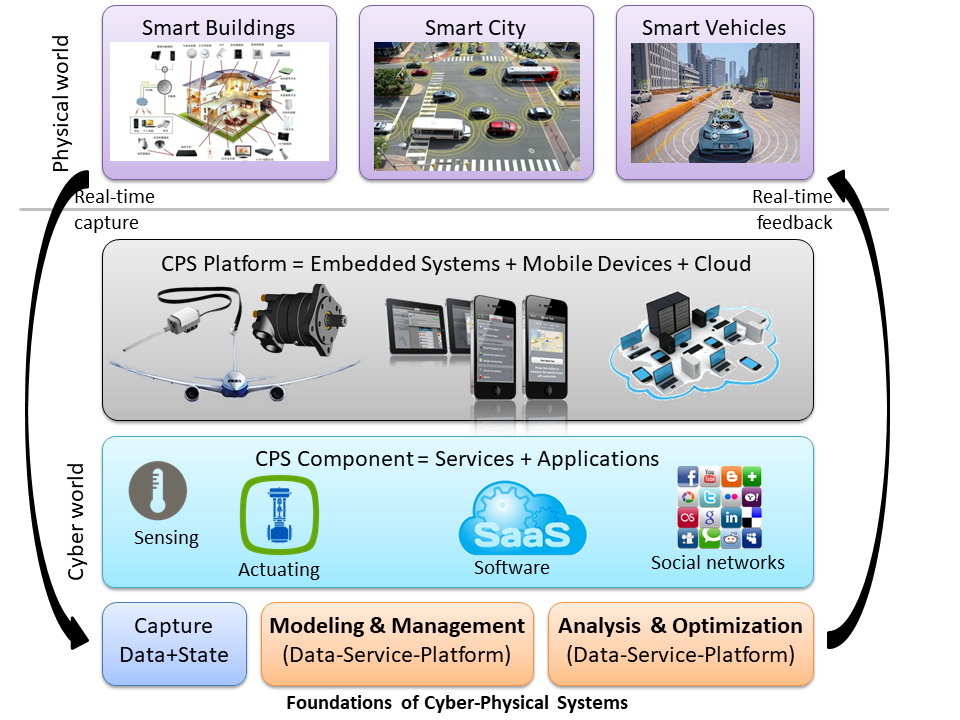
\includegraphics[width=.65\textwidth]{figures/smart-safe-cps}
\caption{Smart and safe cyber-physical systems}
\label{fig:smart-safe-cps}
\end{figure}


\paragraph{Objectives.}
My recent research has been aiming to develop innovative \emph{design, synthesis, management, validation and optimization techniques and tools}  for engineering smart and safe CPSs. In particular, my research group has been working to address two key long-term objectives:

\begin{itemize}
\item \textbf{Long-Term Objective 1}: How to \emph{design and manage} dynamically evolving smart\& safe CPSs to fulfill multi-domain requirements (e.g. consistency, extra-functional or physical)?
\item \textbf{Long-Term Objective 2}: How to \emph{guarantee or validate} that smart\& safe CPS with multi-domain requirements deliver quality of service in an open and changing environment?
\end{itemize}

%\paragraph{Research environment.}
%This research has been carried out in a rather unique and unconventional research environment. In 2015, I successfully acquired a Hungarian prestigious and highly selective Research Chair position funded by the Hungarian Academy of Sciences to run the \href{https://mta.hu/lendulet/az-mta-lendulet-kutatocsoport-halozata-105402}{MTA-BME Lendület Cyber-Physical Systems Research Group}. Here I was main supervisor of five PhD students, but I also provided co-supervision or strategic guidance for six other PhD students (partially affiliated to the project) who are supervised by young faculty members at the Department of Measurement and Information Systems. 
%In response to the increasing direct political influence on academic institutes and research funding imposed by the Orbán Government in Hungary, I joined the Department of Electrical and Computer Engineering at McGill University as a full professor in 2016. Since then, I have been coordinating research of a virtual (trans-Atlantic) group with frequent visits of Hungarian students at McGill.
%
%Furthermore, I was directly involved in strategically shaping proposals for European projects and training networks where IncQuery Labs Ltd was the involved partner.  Along these lines, we achieved the following major results in the past 5-6 years. 

\subsection{Distributed graph queries for runtime monitoring} 

\begin{table}[htb]
\footnotesize
\begin{tabular}{@{}p{5cm}p{11cm}@{}}
\toprule
%\textbf{ECSE 429 Questions} & \textbf{F18} \\ 
%\toprule
Publications &  \cite{sttt-2019-cps,fase2018-cps,wf-iot-2019,models2019-wcet} (all refereed), 1x \textbf{Best Paper Award} 
\cite{fase2018-cps} \\ \midrule
Graduate students at McGill & M. Búr, F. Khan \\ %\midrule
McGill undergraduates (SURE) &  C. Grosdidier \\ \midrule
%Past graduate students &  I. Ráth, Á. Horváth \\ \midrule
MTA-BME Lendület collaborators & A. Vörös \\ \midrule
%Other collaborators & G. Szilágyi, Z. Micskei, L. Balogh, B. Hegyi, B. Horváth, Z. Mázló \\ \midrule
%Key impact &  Publications at leading venues (including ICSE),  \\ \midrule
Funding &  NSERC DG (CA), MTA-BME Lendület (HU), NSERC Engage (under review) \\ %\midrule
\bottomrule
\end{tabular}
\caption{Summary: Distributed graph queries for runtime monitoring}
\end{table}

\paragraph{Motivation.} 
Since upfront formal verification is typically infeasible for smart CPSs, runtime monitoring is a common practice to continuously detect the violation of (safety) properties at runtime. Runtime monitoring has been addressed by runtime verification (RV) techniques %\cite{Leucker2009,Mitsch2014} 
which provide formal precision, but offer a low-level specification language (with simple atomic predicates to capture information about the system). 
%Recent RV approaches \cite{Havelund2015} started to exploit rule-based techniques over a richer (relational or graph-based) information model. 
Runtime models %\cite{BlairBF09,Szvetits2013} 
provide a rich knowledge representation to capture the runtime operational state and context of a smart CPS as typed and attributed graphs to serve as a unifying semantic basis for runtime assurance of self-adaptive systems (SAS).
%in \cite{Cheng2014,Vogel2014}. 
While graph models are widely used internally in various design tools for CPS (e.g. Capella, Artop), real-time CPSs dominantly use low-level data structures with static (i.e. compile-time) memory allocation to ensure resource constraints such as memory limits or deadlines, which is a major limitation.
% Unfortunately, \emph{such static data models are unable to capture dynamically evolving contextual information where there is no a priori upper bound on relevant contextual objects} (e.g. many pedestrians may be in contextual range of a self-driving car), which is a major limitation. 

\paragraph{Results.}
Together with my M. Búr (my PhD student at McGill), G. Szilágyi and A. Vörös, we proposed different graph-based technologies for runtime monitoring purposes in smart\& safe CPS, showcased in the context of the MoDeS3 research demonstrator \cite{nfm2018}. For that purpose, we adapted existing model management and distributed graph query techniques to be deployed over a heterogeneous, decentralized execution platform with resource constraints \cite{fase2018-cps}.  Since graph queries have traditionally been used at design-time by executing them on desktop computers (or servers), their adaptation to a resource-constrained runtime platforms is a highly complex challenge. 
We evaluated the performance of our graph query based runtime monitors \cite{wf-iot-2019} over the DDS (Data Distribution Service) platform, which is a standard of the Object Management Group (OMG). Furthermore, in a very recent journal paper \cite{sttt-2019-cps}, we precisely formalized the behavior of our distributed algorithms and carried out a more extensive scalability evaluation. 
In order to use such graph query techniques for monitoring purposes in hard real-time applications, the worst case execution time (WCET) of the monitoring programs needs to be estimated. Thus in our recent MODELS 2019 paper \cite{models2019-wcet}, we proposed a long-term research agenda and an initial approach that exploits existing WCET analysis tools for calculating WCET for graph queries.

\paragraph{Impact.} 
We published several papers at leading conferences  \cite{fase2018-cps,models2019-wcet} and journals \cite{sttt-2019-cps}. Our paper \cite{fase2018-cps} received an \textbf{EASST Best Paper Award} at ETAPS 2018 (1 award out of over 140 papers). The MoDeS3 framework has been demonstrated at numerous industrial and other public events at BME (e.g. at the annual Researchers Night). These conceptual results have been successfully used in the MoDeS3 open demonstrator for smart and safe CPSs \cite{nfm2018}. I delivered a keynote talk at Ericsson Industrial Day 2016, at the CSCS 2016 Hungarian conference for PhD students, and several invited lectures at the DSM-TP international summer school in several consecutive years. Our results will provide a basis for an upcoming industrial collaboration with Predikat Inc. (Canada) where runtime monitoring of performance degradations in multi-tier web applications will be carried out (the NSERC Engage project is still under review).
% and in an initial prototype developed for the successful Hungarian start-up TeqBall.

\paragraph{My role.}
I was the strategic initiator of this line of research. I was also the main supervisor of M. Búr (PhD student at McGill) and provided strategic guidance for A. Vörös (assistant professor at BME). I contributed to the precise mathematical formulation of the results \cite{fase2018-cps,sttt-2019-cps,models2019-wcet} and also to the textual contents of all publications. I was the PI of a related NSERC Discovery Grant (Canada), an NSERC Engage application and the Lendület Research Group (Hungary). 

\subsection{Automated generation of domain-specific graph models: The CORE-DISC challenge}

\begin{table}[htb]
\footnotesize
\begin{tabular}{@{}p{5cm}p{11cm}@{}}
\toprule
%\textbf{ECSE 429 Questions} & \textbf{F18} \\ 
%\toprule
Publications &  \cite{fmhe2018,sosym2017-dsl,sttt-2019-div,fase2018-diverse,fase2016-solver,icse2018-solver,icse2019-tool,MODELS2016-metrics,MODELS2016-bx,models2018} (all refereed), 2x defended PhD theses (by O. Semeráth, G. Szárnyas) \\ \midrule
Graduate students at McGill & A. Babikian \\ %\midrule
Graduate research trainees at McGill &  O. Semeráth, G. Szárnyas (PhD students defended at BME, supervisor), K. Marussy (PhD student at BME, co-supervisor)  \\ %\midrule
McGill undergraduates (SURE) &  A. Babikian, S. Pilarski, A. Li, B. Chen, L. Li, M. Ding, V. Gidla \\ \midrule
Past graduate students &  G. Bergmann, Á. Horváth \\ \midrule
MTA-BME Lendület collaborators & R. Farkas, A. Vörös \\ \midrule
Other collaborators & Z. Szatmári \\ \midrule
%Key impact &  Publications at leading venues (including ICSE),  \\ \midrule
Funding &  NSERC DG (CA), MTA-BME Lendület (HU) \\ %\midrule
\bottomrule
\end{tabular}
\caption{Summary: Automated generation of domain-specific graph models}
\end{table}

\paragraph{Motivation.}
Graphs are key abstractions in science and engineering. They may represent linked data in graph databases, complex designs of cyber-physical systems or critical contextual situations for autonomous systems. Synthetic graph generators are essential when the use of real graph models is restricted (to respect privacy regulations or intellectual properties of companies) or impractical (to find corner-cases for safety assurance). I initiated the CORE-DISC \emph{long-term research program program} \cite{fmhe2018} to develop a next generation of synthetic graph generator techniques and tools that are customizable to different application domains to derive graph models which are simultaneously \emph{CO: consistent} (graphs shall satisfy various structural logic constraints of the domain), \emph{RE: realistic} (synthetic graphs shall resemble real graphs of a given domain), \emph{DI: diverse} (any pair of graphs shall be structurally distant from each other) and \emph{SC: scalable} (the graph generator shall be able to derive large graph models). Such synthetic graphs are intended to be used as test cases in tool qualification process prescribed by safety standards.% (like DO-330).

\paragraph{Results.} 
As consistency appeared to be the most difficult property to achieve, our initial investigations \cite{fase2016-solver,sosym2017-dsl} aimed to derive consistent graph models with the use of existing logic solvers like Alloy with Kodkod (from MIT) 
%\cite{Torlak2007} 
or Z3 (from Microsoft Research) %\cite{Moura-tacas2008}, 
but none of these attempts were able to scale by failing generate models with over 100 graph nodes. Therefore, we developed a novel \emph{consistent graph solver} \cite{icse2018-solver,icse2019-tool}(with my students, O. Semeráth, A. Nagy, G. Szárnyas, A. Babikian and S. Pilarski) for automatically generating consistent graph models by implementing a novel refinement calculus over partial models \cite{fmhe2018} and using an approximation technique based on constraint rewriting \cite{icmt2017}. Our consistent graph solver \cite{icse2018-solver,icse2019-tool} scales 1-2 orders of magnitude better than competitors that use background logic solvers and its scalability is comparable to search-based techniques %\cite{Soltana2017} 
while uniquely providing both consistency and completeness guarantees. We successfully applied the model generator for incremental backward propagation of view models \cite{MODELS2016-bx} as well as for incremental view model synchronization \cite{models2018}.

Moreover, we provided the first characterization of \emph{realistic models} in \cite{MODELS2016-metrics,fmhe2018} by adapting various graph metrics from network science and evaluating them on graph models taken from six different domains of software and systems engineering. By adapting graph shapes, %\cite{Rensink}, 
we proposed various \emph{model diversity metrics} \cite{fase2018-diverse,sttt-2019-div} by which generalize and subsumes several existing coverage metrics used for testing of model transformations. We extended our model generator and showed that it derives more diverse models than its direct competitors \cite{fase2018-diverse,fmhe2018,sttt-2019-div}. 

%aimed  Generating consistent After a series of initial results , we rea attempts with negative scalabil results 

\paragraph{Impact.}
We published our results in a series of papers at leading conferences and journals of software engineering including 1 book chapter, 1 journal paper at SoSyM \cite{sosym2017-dsl}, 1 at \cite{sttt-2019-div} in Software Tools on Technology Transfer (Springer), 2 papers at MODELS \cite{MODELS2016-bx,models2018}, 2 papers at FASE \cite{fase2016-solver,fase2018-diverse}. I also two invited talks on this topic: one at the CSER 2017 conference in Montreal and one at the Search Based Model Engineering Workshop at King's College London in 2018.
As a special highlight, we published a research paper \cite{icse2018-solver} and a tool paper \cite{icse2019-tool} at ICSE, the prime general-purpose software engineering conference, which is a major success as no modeling papers had been published in the previous three editions of ICSE. 
The news about our ICSE paper \cite{icse2018-solver} was \emph{featured on the front page of the Hungarian Academy of Sciences} (\href{http://mta.hu/english/innovation-of-hungarian-researchers-could-revolutionise-car-industry-design-technology-testing-108434}{Eng}, \href{http://mta.hu/tudomany_hirei/magyar-kutatok-eredmenye-forradalmasithatja-az-autoipari-tervezoeszkozok-teszteleset-108355}{Hun}) and shared by \emph{six major news portals in Hungary}, and I received three invitations for interviews in radio channels. 
%Our approach (published in \cite{sosym2017-dsl,act2017,fmhe2018,fase2018-diverse,icse2018-solver,icse2019-tool}) \emph{scales 1-2 orders of magnitude better} than competitors using state-of-the-art logic solvers like Alloy (MIT) or Z3 (Microsoft Research) and its scalability is comparable to search-based techniques \cite{Soltana2017}. 

%The model generator tool \cite{icse2018,icse2019-tool} provides 1-2 orders of magnitude better scalability compared to exis
%Already the initial results for the formal validation technique for DSLs \cite{models2013} (extended later to the journal paper \cite{sosym2017-dsl}) received Best Paper Award at the IEEE/ACM MODELS 2013. 

\paragraph{My role.}
I was the sole PhD supervisor of key contributors (O. Semeráth, G. Szárnyas, A. Nagy) and MEng students (A. Babikian, S. Pilarski) of this research line, hence being the last author in all papers above. I was the first author of \cite{fmhe2018}, which presents a long-term research agenda and challenges for automated graph model generation. My technical contributions  include some precise foundations and key theorems for the refinement calculus over partial models. I was the PI of the Lendület project and NSERC Discovery Grant that provided funding for the involved students.


\subsection{Secure collaborative modeling}

\begin{table}[htb]
\footnotesize
\begin{tabular}{@{}p{5cm}p{11cm}@{}}
\toprule
%\textbf{ECSE 429 Questions} & \textbf{F18} \\ 
%\toprule
Publications &  \cite{sosym2017-mondo,ieeesw2018,MODELS2016-access,fase2016-merge,esec-fse2017,%
models2017,vlhcc2018,commitmde2016,commitmde2017} (all refereed), 1x PhD thesis (under review), 
1x \textbf{Distinguished Paper Award} \cite{MODELS2016-access}
\\ \midrule
Graduate students at McGill & M. Búr  \\ %\midrule
Graduate research trainees at McGill &  C. Debreceni (PhD student at BME, main supervisor) \\ \midrule
Past graduate students &  G. Bergmann, I. Ráth \\ \midrule
Other collaborators &   De Carlos, X. Mendialdua and S. Trujillo (Ikerlan, Spain), A. Barisic, V. Amaral, M. Goulao (Nova Univ. Lisbon, Portugal) \\ \midrule
Funding &  MTA-BME Lendület (HU), MONDO (EU), NSERC DG (CA), %Bolyai scholarship (HU, secured by G. Bergmann)
 \\ %\midrule
\bottomrule
\end{tabular}
\caption{Summary: Secure collaborative modeling}
\end{table}

\paragraph{Motivation.}
As a common industrial practice in model-based systems engineering, system integrators frequently outsource the development of various components to subcontractors in an architecture-driven supply chain where the collaboration between cross-organizational teams is facilitated by sharing models stored in model repositories. However, effective cross-organizational collaboration is hindered by numerous factors, such as (1) lack of appropriate fine-grained access control management to protect the intellectual property rights (IPR) of involved parties, (2) model fragmentation, or (3) the inability to combine online (GoogleDoc type) and offline (Git or SVN-like) collaboration schemes. 

\paragraph{Results.} 
Together with C. Debreceni, M. Búr, G. Bergmann and I. Ráth, we developed a collaborative modeling framework \cite{esec-fse2017,ieeesw2018} that enhances modeling repositories by providing secure views as an extra protection layer with rule-based high-level access control simultaneously enforced for both offline and online collaboration scenarios and adapted to software configuration management. As a novel underlying concept, we developed a rule-based fine-grained access control technique using bidirectional transformations \cite{MODELS2016-access}. The soundness of the core collaboration scheme was formally proved and successfully applied for both online and offline collaborations in \cite{sosym2017-mondo}. 
Further technical details about the fine-grained model-level access control were published in two peer-reviewed workshop papers \cite{commitmde2016,commitmde2017}. 
To enhance the practical usefulness of the collaborative modeling framework, we developed an automated model merge technique driven by design space exploration \cite{fase2016-merge} (which was evaluated in a collaborative user study \cite{vlhcc2018}). Furthermore, we successfully developed an approach \cite{models2017} to implement the concepts of property-based locking that prevents unintentional model modifications during extensive collaboration. 

\paragraph{Impact.} 
We published seven research papers \cite{fase2016-merge,MODELS2016-access,models2017,esec-fse2017,vlhcc2018,sosym2017-mondo,ieeesw2018} at leading scientific forums (including conferences like MODELS, FASE, ESEC/FSE, VL/HCC and journals like Software and Systems Modeling and IEEE Software). Paper \cite{MODELS2016-access} received \textbf{ACM Distinguished Paper Award} at the MODELS 2016 conference, while the papers above received over 40 citations (Google Scholar). Related concepts were integrated into an innovative product developed by IncQuery Labs Ltd. \cite{models2018-tool}.
%Paper \cite{vlhcc2018} carried out a user study in an industrial setting as part of the MPM4CPS EU COST Action.

\paragraph{My role.} 
I was the strategic initiator of this research line, thus the last author in most related publications (except for the collaborative paper \cite{vlhcc2018}). I am the main supervisor of C. Debreceni and M. Búr who were major technical contributors of the framework. C. Debreceni has already submitted his PhD thesis, and his public defense is expected in Fall 2019. I was the site leader of the MONDO FP7 project at BME where this line of research was started, and the PI of the Lendület project which provided continuity. I helped G. Bergmann (who is an assistant professor at BME) to successfully apply to the prestigious János Bolyai Scholarship in Hungary in a related research topic. 

\subsection{Digital Multidisciplinary Analysis and Design Optimization Platform}

\begin{table}[htb]
\footnotesize
\begin{tabular}{@{}p{5cm}p{11cm}@{}}
\toprule
%\textbf{ECSE 429 Questions} & \textbf{F18} \\ 
%\toprule
Publications &  \cite{mdeintelligence2019} (refereed), 3x MEng thesis (in preparation) \\ \midrule
Graduate students at McGill & M. Rangappa, J. Dhaliwal \\ \midrule
Other collaborators &  M. Staniszewski, Frederic Villeneuve (and other Siemens engineers) \\ \midrule
Funding &  NSERC CRD with Siemens (CA) \\ %\midrule
\bottomrule
\end{tabular}
\caption{Summary: Digital multidisciplinary analysis and design optimization platform}
\end{table}

\paragraph{Context.}
Gas turbines are a commonly used type of internal combustion engine used for power generation. The development of gas turbines requires creation of many different linked models by mechanical engineers. These models are used in gauging performance, designing secondary air systems, combustion, and other subsystems. Creation of design models can span across dozens of design tools which can integrate many data formats, disciplines, and requirements, which introduces significant software engineering challenges. For example, the large number of models inherently results in a huge design exploration space during the development process of an entire engine. Furthermore, the actual tool workflows need to be seamlessly integrated with the underlying development processes.

\paragraph{Results.}
This industrial CRD project started in 2018, and we work on innovative software-as-a-service solutions to integrate various design, analysis and optimization tools driven by workflows. This line of research is carried out together with my McGill MEng students, Maruthi Rangappa, Jasvir Dhaliwal and Sebastian Pilarski, and in collaboration with leading Siemens managers (M. Staniszewski and F. Villeneuve). We aim to develop a cloud-based solution to systematically store and query simulation results to allow fast iterations and a more agile design process. Moreover, we aim to exploit advance machine learning techniques to bring expertise gained from field data and simulated data directly to the mechanical engineers working on engine design. Initial results and a research roadmap has been proposed in \cite{mdeintelligence2019}, while two MEng theses about a graphical workflow editor and an "analysis tool as a service" infrastructure are planned to be submitted by J. Dhaliwal and M. Rangappa in Fall 2019.

\paragraph{Impact.}
While the project is still in an early phase, we made significant technological impact within Siemens. A software prototype developed by Sebastian Pilarski's will serve as the baseline software architecture for a cloud-based simulation environment being developed at Siemens. We also published a joint vision paper with leading Siemens managers at a MODELS 2019 workshop \cite{mdeintelligence2019}. 

\paragraph{My role.}
I am a co-PI of the NSERC project (PI: M. Kokkolaras - McGill, co-PI: H. Moustapha - ETS), and the only software engineering professor in the collaboration. I was contributing to the entire project preparation and proposal writing phase. I am the main supervisor of the three MEng students working on the project. In 2018, I was an invited speaker at the Siemens Industrial Day at ETS (Montreal), and also gave a talk about the project for graduate students.


\subsection{Continuation of previous research lines}
\paragraph{Results.} 
Naturally, I also continued previous research lines started in Stage 1 of my career. Below I summarize and report results where major progress has been made after I joined McGill University. 

\begin{itemize}[leftmargin=0.5cm]
\item
\textbf{Benchmarks for incremental graph queries:}
With key contributions from G. Szárnyas (my PhD student), we prepared a journal paper \cite{sosym2017-tb} to extend the Train Benchmark with a cross-technology comparison of graph query techniques with over 10 tools (including relational databases, graph databases, Eclipse-based modeling tools, rule-based expert systems, etc.). Thanks to the free availability of its source code repository, the Train Benchmark has been actively used by four independent research groups within the model-driven engineering community.


\item 
\textbf{Model transformation techniques:}
Together with O. Semeráth, C. Debreceni (my PhD students), K. Marussy (co-supervised by me) and Á. Horváth, we published two papers at the MODELS conference about the incremental backward synchronization of model transformations \cite{MODELS2016-bx} and fully incremental view model transformations \cite{models2018}. 

\item
\textbf{Design space exploration:}
Thanks to the key contributions from my PhD students, A. Nagy and O. Semeráth, the VIATRA-DSE open source software won \emph{two first prizes at the 9th Transformation Tool Contest} (\href{https://www.transformation-tool-contest.eu/2016/solutions_cra.html}{TTC 2016}). Subsequently, the prototype software was evaluated at NASA Jet Propulsion Lab for high-level mission planning.

\item
\textbf{Formal verification of reactive systems:}
With V. Molnár, Á. Hajdu (graduate research trainees at McGill), B. Graics, A. Vörös, Z. Micskei, I. Majzik (staff members at BME and main supervisors of PhD student), we developed a high-level modeling language for semantically precise composition of reactive components defined by statecharts where each component may follow a different execution semantics (e.g. synchronous vs. asynchronous). The Gamma tool was demonstrated at ICSE 2018 \cite{icse2018-gamma} and the related research paper \cite{sosym-2019-gamma} is under review. I gave an invited talk and a tutorial about this line of research at the DSM-TP 2017 international summer school.


\end{itemize}


\subsection{International research collaborations}

While as a senior researcher, my main mission is to supervise graduate students and help them mature as independent researchers, I still continue participating in international collaborations that typically result in joint publications. Below I summarize a few joint initiatives from the past 3-4 years. 

\begin{itemize}[leftmargin=0.5cm]
\item \textbf{Server-side incremental queries } 
I actively collaborated with researchers and software engineers of IncQuery Labs Ltd. from the inception phase to develop an innovative, server-side product called IncQueryServer for TeamWork Cloud. The product exploits advanced graph query techniques to provide cloud-based server-side validation services over large system models captured in the standard SysML language. The product is  provided as an add-on to a popular cloud-based model repository product of NoMagic/Dassault Systems. We published a joint tool demonstration paper \cite{models2018-tool}, which  received a \textbf{Best Tool Paper Award} at the MODELS 2018 conference.

\item \textbf{Survey on model transformations} In 2017, I was invited to collaborate on a new survey assessing the state of the art of model transformation tools with N. Kahani, M. Bagherzadeh, J. Cordy and J. Dingel (all from Queen's University). The collaboration resulted in a joint paper \cite{sosym2019-mt} published at the SoSyM journal in 2019 and it already received 10+ independent citations.

\item \textbf{Complex event processing for runtime models}
As a continuation of past research \cite{models2014-stream} carried out with I. Dávid (Univ. Antwerp, Belgium) and I. Ráth to adapt the concepts of complex event processing for runtime models for stream processing, we published an extended journal version of our results which contained precise formalization of our concepts \cite{sosym2018-cep}. Certain concepts along this line were used in a proof-of-concept prototype developed for the successful Hungarian start-up TeqBall.

\item \textbf{User study on model merge techniques} 
Together with A. Barisic, V. Amaral, M. Goulao (researchers at Nova Univ. Lisbon, Portugal) and my PhD student C. Debreceni, we collaboratively carried out and published a user study \cite{vlhcc2018} to assess the usability of a novel model merge technique. In fact, the model merge technique \cite{fase2016-merge} was also a result of collaborative research within the MONDO project with X. De Carlos, X. Mendialdua and S. Trujillo (from Ikerlan, Spain). The execution of user study was mainly driven by the collaborators from Portugal (and partially supported by MPM4CPS EU COST Action), while we provided technical support for the focal tool of the user study. 
\end{itemize}


\section{Future Research}

%\subsection{Context}

\paragraph{Motivation.} 
Digitalization is a dominating trend in engineering in initiatives like Industry 4.0 or Internet-of-Things. The concept of \emph{digital twins} (i.e. digital replica of physical assets, processes, people, places, systems) requires developing and continuously maintaining a digital representation of design documents in the form of models using a multitude of design, validation and optimization tools. The traditionally separate design and operation phases are blurred by systematically recording operational (field) data and processing it by machine learning and software engineering techniques to provide useful input for next design cycles. Decision making in autonomous CPSs (like self-driving cars, or drones) relies upon runtime models collected by a network of sensors, and fused by various artificial intelligence techniques. 

\paragraph{Main challenge.}
While innovation for digitalization is driven by software and intelligent data processing techniques; however, there is too much optimism for their fast penetration to critical CPSs (like cars, aircrafts, space) while appropriate means of quality assurance is severely lacking, especially in the presence of an increased level of automation or autonomous behavior.
 
%\begin{itemize}
%\item[(1)] 
While dozens of software tools are necessitated to a fully digital design of a complex CPS, quality assurance for tools and integrated tool chains is insufficient and represents a major risk for digitalization. How to trust a digital twin if one cannot trust the software tool used for designing it? Software safety standards of critical avionics systems (\href{https://standards.globalspec.com/std/1461615/rtca-do-330}{DO-330}) prescribe that only the output of a qualified tool can be trusted, and such a tool should meet the same requirements as the critical system component it designs. However, it makes tool qualification extremely costly.

%\item[(2)]
Due to recent fatal accidents, the safety assurance of autonomous cyber-physical systems (like self-driving cars or autonomous drones) is still its infancy. Unfortunately, decades of verification and validation (V\&V) practices developed for traditional safety-critical software systems are not applicable to autonomous systems. Existing practices rely up exhaustive simulation for system validation, but statistical techniques do not provide sufficient level of dependability and coverage in case of extremely rare events where one combination of rare events may jeopardize safety.
%\end{itemize}

\paragraph{Objectives.}
As a high-level objective, my ongoing and future research aims to increase the level of trust in digitalization for CPSs by developing systematic validation techniques for design tool chains and autonomous systems by automatically synthesizing potentially unsafe or problematic corner-cases and contextual situations. While the potential of digitalization is unquestionable, this project will mitigate its risks and negative impacts.

In particular, I am interested in novel scientific foundations and scalable software tools for 
\begin{enumerate}
\item the integration and testing of design tools used in digitalization for CPS, 
\item the system-level assurance of autonomous CPS,
\item the systematic testing for intelligent CPS driven by machine learning. 
\end{enumerate}

\paragraph{System-level assurance of autonomous CPS}
%\paragraph{Key ideas.}
Since safety-critical autonomous vehicles need to interact with an immensely complex and continuously changing environment, their assurance is a major challenge, and upfront design time assurance is generally regarded to be practically infeasible. While systems engineering practice necessitates assurance on multiple levels,  existing research focuses dominantly on component-level assurance while neglecting complex system-level traffic scenarios.
Our research aims to address the system-level testing of the situation-dependent behavior of autonomous vehicles by combining various model-based techniques on different levels of abstraction. Major initial progress and a research roadmap (developed in a SURE project in Summer 2018 and later in collaboration with researchers from BME but still under my scientific leadership) is reported in a vision paper \cite{models2019-systest} accepted at the MODELS 2019 conference.

%(1) Safety properties are continuously monitored in challenging test scenarios (obtained in simulators or field tests) using graph query and complex event processing techniques.  (2) To precisely quantify the coverage of an existing test suite with respect regulations of safety standards, we provide qualitative abstractions of causal, temporal, or geospatial data recorded in individual runs into situation graphs, which allows to systematically measure system-level situation coverage (on an abstract level) wrt. safety concepts captured by domain experts.  (3) Moreover, we can systematically derive new challenging (abstract) situations which justifiably lead to runtime behavior which has not been tested so far by adapting consistent graph generation techniques, thus increasing situation coverage. (4) Finally, such abstract test cases are concretized so that they can be investigated in a real or simulated context.

%\begin{enumerate}
%\item Safety properties are continuously monitored in challenging test scenarios 
%(obtained in simulators or field tests) using graph query and complex event processing techniques.  
%\item To precisely quantify the coverage of an existing test suite with respect regulations of safety standards, we provide qualitative abstractions of causal, temporal, or geospatial data recorded in individual runs into situation graphs, which allows to systematically measure system-level situation coverage (on an abstract level) wrt. safety concepts captured by domain experts. 
%\item Moreover, we can systematically derive new challenging (abstract) situations which justifiably lead to runtime behavior which has not been tested so far by adapting consistent graph generation techniques, thus increasing situation 
%coverage. 
%\item Finally, such abstract test cases are concretized so that they can be investigated in a real or simulated 
%context.
%\end{enumerate}

%\subsection{Testing of data sets used for machine learning in CPS design}
%
%\paragraph{Objectives.} Even when a large amount of field data is available as a training set, machine learning techniques provide no guarantees that this training set covers particular corner cases and rare events. We plan to devise an iterative and incremental approach which continuously evaluates a training set with respect to some coverage criteria over an abstract (graph-level) equivalence class, and then uses a graph generator (see below) to systematically derive test data for uncovered partitions of training data.
%
%\subsection{Auto-generation of consistent, realistic, diverse and scalable models}
%\paragraph{Objectives.} As a cross-domain underlying research line, we aim to develop automated synthetic graph generators with precise foundations, efficient algorithms and open-source scalable software prototype implementation to derive domain-specific graph models which are \emph{simultaneously consistent, realistic, diverse and scalable}. 
%Since graphs provide key abstractions of complex information in science and technology (including  design and runtime information of complex, software-intensive CPS), auto-generated graph models can serve as test cases or benchmarking purposes, especially, in data intensive, decentralized applications.

\section{Research Funding}

\subsection{Past research funding (Stage 1)}
In the first stage of my career, I was successful in attracting a variety of substantial research funding with both individual and collaborative research projects, with academic as well as industrial funding. 

\paragraph{Collaborative European projects: }
Since 2005, I was the site leader or research coordinator at BME for a series of collaborative European projects. The \emph{SENSORIA project} (2005-2010) aimed to provide precise software engineering techniques for next-generation service-oriented overlay computers. The \emph{DIANA project} (2006-2010) involved large avionics companies to provide a distributed and equipment-independent environment for avionics applications compliant with the ARINC 653 standard. The E-Freight project (2010-2013) aimed to improve on European e-freight capabilities for combined transport routes. The SecureChange project (2009-2012) developed various security engineering techniques used for evolving software-intensive systems. Finally, the MONDO project (2013-2016) was concerned with the development of scalable modeling and model management techniques deployed over a cloud platform.
I was involved in these projects starting both during the proposal writing as well as the actual execution phase. I was the scientific leader for different work packages, coordinated the development of project demonstrators, and altogether, I successfully collaborated with well over 100 researchers in Europe.

\paragraph{Individual research grant applications: }
I was also successful in grant applications where I was the sole PI. In particular, my ERC Starting Grant project (CERTIMOT: Design and Analysis Techniques for Certifiable Model Transformations) went to the final round of reviews at the European Commission with a supportive score of 7/8, but it became out of budget. Finally, it received partial funding from the Hungarian Research Agency and ran between 2010 and 2014. My application to the MTA Lendület research chair program is detailed below.


\paragraph{Industrial funding: }
I was the principal investigator of a two-year research project (TRANS-IMA) funded by Embraer, the large Brazilian airframer to develop innovative model-based avionic tools for their systems engineering process (total funding: 200,000 EUR). Previously, I was the three times recipient of the IBM Faculty Award offered by IBM TJ Watson Research Center (total amount of 36,000 USD). I was research coordinator for two collaborative projects with Nokia Research Centre (Budapest) on high-availability service platforms and model-driven development techniques (approx. 40,000 EUR).

\subsection{Recent research funding (Stage 2)}
Since 2015, I successfully continued to secure substantial amount of research funding with a total amount of Canadian funding over 1.46 million CAD as PI or co-PI (own share of funding: 580,000 CAD), and additional own funding over 160 million HUF (equivalent of over 730,000 CAD) in Hungary. Except for my start-up grant offered by McGill University, all other grants were secured on a competitive basis. Further financial details of funding are listed in my CV.

\paragraph{NSERC CRD: Digital Multidisciplinary Analysis and Design Optimization Platform (2018-2023): }
We started a 5-year long multidisciplinary collaborative research and development (CRD) project co-funded by Siemens Canada and NSERC targeting a design platform for designing aeroderivative gas turbines. The total funding of the project is around 1.2 million CAD (with roughly 25\% is reserved to my own research). 

%Furthermore, I gave two invited talks at the Siemens-ETS Industry 4.0 Day in Montreal in 2018. 

\paragraph{NSERC Engage (2019-2020): Automated identification of performance regressions in a multi-tier web applications, under review}
With its innovative Predicate AIOps tool suite, our industrial partner, Predikat Inc. offers innovative solutions to prevent down-time and predict traffic for multi-tier web applications for companies providing business-critical
Software-as-a-Service solutions deployed over virtual machines or as microservices using a complex,
multi-layered software stack composed of heterogeneous technologies. As a specific problem at Predikat,
finding the root cause of identified performance regressions is a time-consuming manual task. This project
aims to identify performance bottlenecks in multi-tier web applications by runtime monitoring and then provide
automated root cause analysis to trace the bottleneck to the relevant component in real-time, thus removing the
burden of manual troubleshooting from DevOps engineers. As such, it would further enhance the existing
capabilities of the Predicate AIOps tool suite. The project is under evaluation, and it is expected to run for six months starting in Fall 2019.

\paragraph{NSERC Discovery Grant (2016-2021): Model-based Design and Validation Techniques for Smart and Safe
Cyber-Physical Systems:}
Due to its flexible nature, my NSERC Discovery Grant provided funding for students without having an industrial project. This included Márton Búr (PhD student at McGill), and Faizan Khan (MEng student at McGill) to carry out research in the context of Internet-of-Things applications of cyber-physical systems. In addition, it funded a total of 9 undergraduate students who participated in early research activities as part of the Summer Undergraduate Research in Engineering (SURE) program. Furthermore, travel costs of several Hungarian PhD students who visited my as McGill graduate research trainees were covered.

\paragraph{LiveIDE: Live Integrated Development Environment for Software-Intensive Communication Systems (2017): }
In 2017, I led the submission of a proposal as principal investigator for a three-year NSERC Strategic Partnership Grant for Projects with G. Mussbacher, J. Kienzle (McGill), H. Sahraoui and E. Syriani (UdeM) as co-PIs and Ericsson Montreal as supporting industrial partner. NSERC offered to accept the project without further changes as a collaborative research and development (CRD) project due to its industrial relevance, but unfortunately, this CRD contract was not signed as the main contact and project lead at Ericsson left the company (after 20 years).

\paragraph{MTA-BME Lendület Cyber-Physical Systems Research Group (2015-2020)}
This prestigious and highly selective research chair program is run by the Hungarian Academy of Sciences, and each year a total of 12-15 researchers below the age of 45 are awarded nation-wide. In 2015, I was only the third ever recipient in the field of computer science. The project provided partial funding for 10 PhD students and 2 junior staff members at BME to do research on various challenges of cyber-physical systems.

%\paragraph{Further initiatives for research funding:}
%In addition, I was actively seeking further opportunities for research funding, being the PI for a proposal for the 
%MSSI (McGill Sustainability Systems Initiative) Ideas fund (Sustainity: A Knowledge Base for Sustainability Research) with G. Mussbacher (McGill) as co-PI, and being the co-PI in in an application submitted in the NSERC Collaborative Research and Training Experience (CREATE) program (TRANSMIT: Training program in continuous software migration to emerging technologies), and a co-PI in a proposal for the IDEaS Innovation for Defence and Security Program (Enhanced Human-Robot Collaboration with Wearable Technology) with G. Beltrame (Polytechnique), A.M. Cretu (Carleton), E. Coffey (Concordia) as PIs. Unfortunately, these initiatives did not receive funding in the respective competitions. 

%\newrefcontext{extref}
%\printbibliography[heading=subbibliography,notcategory=own,title=External references]

\chapter{Service Portfolio}
\label{sec:service-portfolio}
\lfoot{Service Portfolio} 
%\rfoot{Service Portfolio} 

\section{Service for Scientific and Professional Communities}

%\subsection{Summary of service for scientific communities (entire career)}


\subsection{Conference \& workshop organization, Editorial boards}

As a reflection of my reputation in my research area, I served in various key organizational roles for leading scientific conferences and journals after joining McGill University in 2016. 

\begin{itemize}[leftmargin=0.5cm]
\item \textbf{Program co-chair}: Together with Emilie Balland, we served as the program co-chairs of the \emph{9th ACM SIGPLAN Int. Conf. on Software Language Engineering} (\href{https://www.sleconf.org/2016/}{SLE 2016}) hosted in Amsterdam, Netherlands. The SLE conference is devoted to the principles of software languages: their design, their implementation, and their evolution. As a PC co-chair, I was in charge of preparing the call for papers of the conference, organizing the entire review process to ensure the fair evaluation of papers, making decisions on the final selection of papers included in the conference program, assembling the different sessions of the conference, inviting session chairs, etc. 

\item \textbf{Program co-chair}: With with Marsha Chechik and Daniel Strüber, we served as the program co-chairs of the \emph{11th Workshop on Modelling in Software Engineering} (\href{https://sselab.de/lab2/public/wiki/MiSE/index.php}{MiSE’2019}) hosted by ICSE 2019 in Montreal, Canada. This 2-day workshop is a traditional satellited event of the ICSE conference, and it is regarded almost as a conference by the software and systems modeling community. My duties in the organization included to prepare the workshop proposal (as even workshop selection is competitive), organizing the review process for the conference, etc.

\item \textbf{Program board member}: I served on the program board (consisting of 13 senior researchers of the community to overview the review process) in 2016 and 2017 for the \emph{IEEE / ACM Int. Conf. on Model Driven Engineering Languages and Systems} (\href{http://modelsconference.org/}{MODELS}), which is the main scientific forum of my research area. In this role, I was coordinating the review process of papers assigned to me and helped make final decisions on those papers.

\item \textbf{Posters co-chair}: Together with Wahab Hamou-Lhadj, I served as a co-chair of the \emph{Posters Track of the 41st Int. Conf. on Software Engineering} 
(\href{https://2019.icse-conferences.org/track/icse-2019-Posters}{ICSE 2019}), which is the flagship conference on software engineering. In this role, I was contributing to organizing the review process of poster submissions, collaborating with co-chairs of other ICSE tracks, establishing a selection committee, etc.

\item \textbf{Steering committee member}: I continued to serve on the steering committee (SC) of the \emph{Int. Conf. on Model Transformation} (\href{http://www.model-transformation.org/}{ICMT}), which is the major topical conference of my direct research area. My duties included the strategic planning of future editions of the conference (e.g. selecting program chairs and locations) and providing further strategic guidance.

\item \textbf{Editorial board member}: I continued to serve on the editorial board of the \emph{Software and Systems Modeling} (\href{http://sosym.org/}{SoSyM}) journal (Springer), the main scientific journal of my research area. In this role, I am in charge of organizing the review of 1-3 papers each year by selecting qualified reviewers and making recommendations on acceptance or rejection based upon reviewers' feedback.

\item \textbf{Editorial board member}: I was invited to joined the editorial board of \emph{Journal of Object Technology} (\href{http://www.jot.fm/}{JOT}),  a peer-reviewed, free and open-access journal included by all major indexing services. 
\end{itemize}

\paragraph{Entire career}
During my entire career, I served practically in all major roles in the organization of scientific conferences. %Here I provide a 1-paragraph brief summary of the highlights of my academic roles. 
I was \emph{program co-chair} of three major software engineering conferences (FASE 2013, ICMT 2014 and SLE 2016) as well as numerous workshops. I was the \emph{general chair} of the first ever STAF conference (Software Technologies: Applications and Foundations) in 2013, the Fourth Int. Symposium on Applications of Graph Transformations with Industrial Relevance (AGTIVE 2011) and the SENSUS 2009 international summer school. I was \emph{workshops co-chair} at STAF 2016, \emph{doctoral symposium co-chair} at STAF 2015.
%At the IEEE / ACM Int. Conf. on Model Driven Engineering Languages and Systems (MODELS), which is 
At the main scientific venue of my research field, I was \emph{demos and exhibitions chair} at MODELS 2012, academic posters and demos chair at MODELS 2007.  I was the \emph{local organizing chair} of European Joint Conferences on Theory and Practice of Software (ETAPS 2008) with 670 participants and \emph{served on the ETAPS steering committee} for a total of six years. 
I served on the \emph{editorial board of the SoSyM journal}, the main scientific journal of my research area since 2011.  

\subsection{Program committees and further reviewing activities}
Since joining McGill University in 2016, I have continuously received invitations to serve as a reviewer in different program committees (PCs), project evaluation boards or in journals, especially, in the field of software engineering and formal methods. 

\begin{itemize}[leftmargin=0.5cm]
\item \textbf{PC member at ICSE:}
For the first time in my career, I was invited to \emph{serve on the program committees of ICSE 2018 and ICSE 2019}, the IEEE/ACM Int. Conf. on Software Engineering, which is the main scientific forum of software engineering. My thorough reviewing activities were recognized by the prestigious \textbf{ACM Distinguished Reviewer Award} for ICSE 2018 (only 11 awardees out of 101 PC members). 

\item \textbf{PC member at MODELS:}
For the IEEE / ACM Int. Conf. on Model Driven Engineering Languages and Systems (MODELS), which is the main scientific forum of my research area, I served on the Program Board (consisting of 13 senior researchers of the community to overview the review process and make final decisions on papers) in 2016 and in 2017 and on the program committee in 2018 and 2019. 

\item \textbf{PC member at other major conferences:}
I also served on the program committee of other major %software engineering 
conferences including the 
Int. Conf. on Model Transformation (ICMT 2017 and 2018), the European Conf. on Modelling Foundations and Applications (ECMFA 2018 and 2019), the Tools Track of the IEEE Automated Software Engineering Conf. (ASE 2016), Fundamental Approaches to Software Engineering (FASE 2017 and 2018). I also got PC invitations for conferences in the area of \emph{formal methods}.

\item \textbf{Invitation to NSERC Discovery Grant evaluation committee:}
In August 2019, I received an invitation to serve in the \emph{Computer Science Evaluation Group} of the NSERC Discovery Grant program for a three-year term. 
%As the main review period coincides with my heavy teaching workload in the Winter 2020, I decided to decline this invitation 

\item \textbf{Project proposal reviewer:}
I served as an external evaluator of various project proposals including 1x VICI grant from Netherlands, 1x EU COST Action, 1x NSERC Discovery Grant, 16 Bolyai Scholarship applications in Hungary, 1x Women for Science proposal for the Hungarian Academy of Sciences. I also had to decline 3 further review invitations due to conflict of interest.

\item \textbf{Journal reviewer:}
I regularly reviewed for major scientific journals of my research area (software engineering, formal methods) including 4 papers at IEEE Transactions on Software Engineering, 2x for Formal Aspects of Computing, 2x for Software and Systems Modeling, 1x for IEEE Software). Please also note that it is my regular practice to "constructively decline" journal review invitations and recommend my former graduate students as qualified reviewers for the same paper. I strongly believe that this practice helps their integration to the scientific community. 
\end{itemize}

\paragraph{Entire career}
I served on the program committee of leading international conferences and workshops in different research fields: 66 times in software engineering, 16x at visual modeling techniques and tools, 14x at formal methods, 4x at depedendable computing. I served on the senior program board of the MODELS conference twice. I acted as an external evaluator of project proposals in 7 different countries and an external reviewer of tenure / promotion dossiers submitted in UK, Canada and South Africa. 

\subsection{Standardization activities}
In December 2017, the Object Management Group (OMG) issued a Request for Proposal (RFP) for SysML V2, the next-generation systems modeling language standard. In 2018, I regularly participated in the standardization activities of the so-called SST submission group, which is a very large group of companies and universities collaborating to define the next generation of the standard (including e.g. Boeing, Airbus, NASA Jet Propulsion Lab, Siemens, etc.).

As a representative of IncQuery Labs Ltd. (the start-up company I co-founded in Hungary), I partcipated in three in-person meetings of the standardization group (in Boston, June 2018, in Ottawa, September 2018 and in Seattle in December 2018) and several teleconferences. My specific role was related to defining a query language and an open application programming interface (API) for SysML models. In particular, the envisioned query language should be build on the VIATRA Query Language, which is an the open source graph query language based on past research led by me. While the official submission deadline of the related standard is only in Spring 2020, even the potential transition of our query language to the systems engineering standard modeling language is a major impact of our past research activities. 

\section{University Service}
\label{sec:university-service}

\subsection{University-related review activities}
I was very active in university-related review activities both at McGill University and on an international level. Within McGill, I served as the \emph{internal examiner} of 2 PhD theses, a \emph{member of the oral PhD committee} once, and acted as Pro-Dean once. In addition, I was the sole \emph{thesis examiner} of 4 MEng/MSc thesis at McGill. In addition, I served as a \emph{member the qualifying exam committee} for 2 PhD students at McGill. 
At an international level, I was invited to serve as an \emph{external reviewer} of several PhD theses, once in Austria, once in Germany and once in UK. In addition, I served as an examiner and the chair of the complex exam committee at BME in Hungary. 

\paragraph{Entire career}
During my entire career, I was inivited to serve as an expert (i.e. reviewer or committee member) in a total of 24 PhD defenses (7 of which since joining McGill) in 9 different countries while acting as the chair of the PhD defense committee once. 

\subsection{Departmental, faculty and university-level committees}
During the 3 years working at McGill University, I served on 8 different committees for the ECE Department, and 1 working group for the Faculty of Engineering, while acting as an elected representative of the Faculty of Engineering for the Council of Graduate and Postgraduate Studies (CGPS). I served as a member of the Search Committee of the ECE Department for two consecutive hiring rounds (2018 and 2019) evaluating application packages of hundreds of applicants. 
%I serve as the program director of the upcoming software engineering co-op program, which is further detailed as part of my Teaching Portfolio.

%\begin{description}
\begin{yearlist}
\item[2018-19] \textbf{Program director for software engineering co-op}: 
I serve as the program director of the software engineering co-op program (expected to start in Fall 2020) where undergraduate students will need to spend four compulsory internship terms at companies. In that role, I have been working on the key policies, guidelines, student and employer evaluation forms related to the co-op terms since Fall 2018 together with Ms. Lorraine Donald (Industry Liaison Associate at the Faculty of Engineering, and future program coordinator). 
% for the software engineering co-op program). 
Since more than 500 undergraduate students need to find a 3-4 month long internships placements at companies each year, my initiative has been to invest in software-based automation of the key business processes of students going on co-op terms. Another key initiative of mine was was to develop a prototype system for handling co-op terms as the group project of the Winter 2019 edition of the ECSE321 course. This initiative was a major success and projects were demonstrated in front of several McGill employees who currently manage 
co-op programs. 

%Furthermore, I have also been voluntarily participating in the pilot project aiming to install and host GitHub Enterprise on McGill premises (i.e. a private installation of the popular version control system), and I provided valuable feedback to the working group during the W18 edition of the ECSE321 course.


\item[2017-19] \textbf{Faculty of Engineering representative of the Council of Graduate and Postdoctoral Studies (CGPS)}: The mandate of the university-level CGPS council is to evaluate proposal made to different graduate-level programs proposed by the different faculties. As an elected representative of the Faculty of Engineering, I am in charge of assessing and voting about such proposals. In addition, I also need to report about engineering-related discussions and changes in the graduate programs at the Faculty Council meetings. 
\item[2018-19] \textbf{Curriculum Committee member, ECE}: 
This committee is responsible for the maintenance and renewal of the department’s undergraduate programs in Electrical Engineering, Computer Engineering, and Software Engineering. My main contributions are related to introducing specialization streams (i.e. consistent groups of elective courses taken by students) for the Software Engineering program. I also proposed changes to the sample Software Engineering curriculum of the upcoming co-op program, especially, with respect to the scheduling of the compulsory co-op terms. Since the SE coop program did not finally start in Fall 2019, the final approval of these proposals were postponed to Fall 2019.

\item[2018-19] \textbf{Undergraduate Advising Committee member, ECE}: 
The mandate of this committee is to provide advising for undergraduate students about anything related to their studies. 
In this role, I provided advise for undergraduate students on course selection, program planning, resolving their scheduling conflicts, and other issues intensively at the first three weeks of each semester, and on an appointment basis afterwards. 


\item[2018-19] \textbf{Student Exchanges \& Study Abroad Committee member, Faculty of Engineering}: I am the ECE representative of this faculty-level committee which promotes and coordinates various international exchange opportunities activities for undergraduate and graduate students. During the year, I was supporting the committee's decision to increase its mandate to other forms of experiential learning. 
\item[2017-19] \textbf{Departmental Search Committee member, ECE}: The mandate of this committee is to make recommendations for the department chair on which candidate to hire for an open professor position. My duties included to attract strong software engineering candidates (e.g. personal contacts or on mailing lists), to rank hundreds of application packages, to discuss applications with other committee members, to assess long-listed candidates via dozens of Skype interviews, to attend several hiring seminars, and to interact with the candidates in person to know their deeper personal and social context.
\item[2017-19] \textbf{GitHub Enterprise Working Group member, Faculty of Engineering}: This working group was in charge of running a pilot project on evaluating the use of the enterprise version of the popular GitHub version control system hosted locally at McGill premises. My main contribution was to voluntarily use the software for the software team projects as part of the ECSE 321 Introduction to Software Engineering course, and provide feedback about its use during the monthly meetings of the working group. A key insight provided by me was that this academic version of GitHub Enterprise is not compatible with academic licenses of other cloud-based software engineering products used for continuous integration (e.g. Travis CI).
\item[2016-18] \textbf{Chairman's Advisory Committee member}: This committee is composed of senior professors of the ECE department, and its mandate is to provide strategic advice for the department chair. My contribution was to highlight strategic areas in software engineering which are not sufficiently covered by existing professors, such as software security. These areas were used by the Departmental Search Committee when evaluating candidates for academic positions at subsequent years.
\item[2017-18] \textbf{Promotions and Reappointments Committee member}: This committee evaluates the compulsory third year report of tenure-track professors and makes suggestions for the feedback provided by the department chair. I was involved in reading and evaluating the report of one tenure-track professor of the ECE department. 
\item[2016-17] \textbf{Departmental Tenure Committee member, ECE}: This committee provides the first round of evaluation of the tenure dossiers of tenure-track professors at the ECE Department. Accidentally, there were no candidates for tenure consideration in the given year, thus there were no specific duties on my side. 
\item[2016-17] \textbf{Graduate Student Financing Committee, ECE}: This committee ranks graduate students for awards and scholarships. My contributions included to rank NSERC Masters applications, NSERC doctoral applications, and Ph.D. students for the McGill Engineering Doctoral Award (MEDA) and to discuss the ranking with other committee members.
\end{yearlist}
%\end{description}

\subsection{International academic committees}
At an international level, I am an elected member of the Informatics Committee (with a total of 15 members) at the Hungarian Academy of Sciences. The committee is in charge of evaluting profiles of senior applicants to the Doctor of Science degree in Hungary (which is a formal prerequisite of promotion to full professorship in Hungary). I have been elected three consecutive times, last time 2017. I remained as a core member of the Informatics Doctoral School at the Budapest University of Technology and Economics (BME). Moreover, I served as an external member of the Informatics Doctoral School at the University of Szeged until the end of 2016.


 



\appendix
\chapter{Sample Publications}
\label{sec:sample-publications}
\lfoot{Sample Publications}
%\rfoot{Sample Publications}


This appendix contains a selection of eight publications from my Publication List (\autoref{sec:publication-list}), which are representative of the high-quality research I conducted at McGill University. The list includes 
\begin{enumerate}[leftmargin=0.5cm]
\item one paper with Márton Búr as first author who is the PhD student I supervise at McGill, 
\item five papers having McGill GRTs (Hungarian PhD students) as first author who I supervised or co-supervised;
\item one tool paper with two McGill undergraduates as co-authors (who are my graduate students since January 2019);
\item one paper prepared in collaboration with other leading researchers of my field.
\end{enumerate}

\vspace{1cm}

{\small
\begin{yearlist}
%\item[\cite{sttt-2019-cps}] M. Búr*, G. Szilágyi, A. Vörös, and D. Varró. “Distributed Graph Queries Over Models\@run.time for Runtime Monitoring of Cyber-Physical Systems”. In: Software Tools on Technology Transfer (2019). In press, pp. 1–25. 
\item[\cite{fase2018-cps}] 
M. Búr*, G. Szilágyi, A. Vörös, and \underline{\textbf{D. Varró}}. “Distributed Graph Queries for Runtime Monitoring of Cyber-Physical Systems”. In: Fundamental Approaches to Software Engineering, 21st International Conference, FASE 2018, Held as Part of the European Joint Conferences on Theory and Practice of Software, ETAPS 2018, Thessaloniki, Greece, April 14-20, 2018. Vol. 10802 of LNCS.  Springer, 2018, pp. 111–128. 
\newline \textbf{EASST Best Paper Award at ETAPS 2018:} 1 out of over 140 papers.
\newline DOI: \href{https://doi.org/10.1007/978-3-319-89363-1_7}{10.1007/978-3-319-89363-1\_7}.

%\item[\cite{}]
%G. Bergmann, C. Debreceni*, I. Ráth, and D. Varró. “Query-based access control for secure collaborative modeling using bidirectional transformations”. In: Proceedings - 19th ACM/IEEE International Conference on Model Driven Engineering Languages and Systems, MODELS 2016. \textbf{ACM Distinguished Paper Award},
%Acceptance rate: 23.7\%. ACM, 2016, pp. 351–361. DOI: 10.1145/2976767.2976793.

%\item[\cite{models2019-wcet}] M. Búr* and \underline{\textbf{D. Varró}}. “Towards WCET Estimation of Graph QueriesRun.time”. In: 21st ACM/IEEE International Conference on Model Driven Engineering Languages and Systems, MODELS 2019, Munich, Germany, September 18-20. In press. ACM, 2019, pp. 1–6.

\item[\cite{sosym2017-mondo}]
C. Debreceni*, G. Bergmann, I. Ráth, and \underline{\textbf{D. Varró}}. “Enforcing fine-grained access control for secure collaborative modelling using bidirectional transformations”. In: Software \& Systems Modeling 18 (3 2019). pp. 1737–1769. 
\newline DOI: \href{https://doi.org/10.1007/s10270-017-0631-8}{10.1007/s10270-017-0631-8}.

\item[\cite{icse2018-solver}] 
O. Semeráth*, A. S. Nagy*, and \underline{\textbf{D. Varró}}. “A graph solver for the automated generation of consistent domain-specific models”. In: Proceedings of the 40th International Conference on Software Engineering, ICSE 2018, Gothenburg, Sweden, May 27 - June 03, 2018. ACM, 2018, pp. 969–980. 
\newline DOI: \href{https://doi.org/10.1145/3180155.3180186}{10.1145/3180155.3180186}.


\item[\cite{ieeesw2018}]
C. Debreceni*, G. Bergmann, I. Ráth, and \underline{\textbf{D. Varró}}. “Secure Views for Collaborative Modeling”. In: IEEE Software 35.6 (2018). IF: 2.190, pp. 32–38. 
\newline DOI: \href{https://doi.org/10.1109/MS.2018.290101728}{10.1109/MS.2018.290101728}.

\item[\cite{sosym2017-tb}]
G. Szárnyas*, B. Izsó*, I. Ráth, and \underline{\textbf{D. Varró}}. “The Train Benchmark: cross-technology performance evaluation of continuous model queries”. In: Software \& Systems Modeling 17.4 (Jan. 2018). , IF: 1.722, pp. 1365–1393. 
\newline DOI: \href{https://doi.org/10.1007/s10270-016-0571-8}{10.1007/s10270-016-0571-8}.

\item[\cite{models2018}]
K. Marussy*, O. Semeráth*, and \underline{\textbf{D. Varró}}. “Incremental View Model Synchronization Using Partial Models”. In: 20th ACM/IEEE International Conference on Model Driven Engineering Languages and Systems, MODELS 2018, Copenhagen, Denmark, October 14-19, 2018. Acceptance rate: 28\%. ACM, 2018, pp. 323--333. 
\newline DOI: \href{https://doi.org/10.1145/3239372.3239412}{10.1145/3239372.3239412}.

\item[\cite{icse2019-tool}]
O. Semeráth*, S. Pilarski*, A. Babikian*, and \underline{\textbf{D. Varró}}. “VIATRA Solver: A Framework for the Automated
Generation of Consistent Domain-Specific Models”. In: 41st ACM/IEEE International Conference on Software
Engineering: Companion Proceedings, ICSE 2019, Montreal, Canada. IEEE, 2019, pp. 43–46. 
\newline URL: \url{https://dl.acm.org/citation.cfm?id=3339687}.

%\item[\cite{icse2018-tool}]
%V. Molnár*, B. Graics, A. Vörös, I. Majzik, and D. Varró. “The Gamma statechart composition framework: design, verification and code generation for component-based reactive systems”. In: Proceedings of the
%40th International Conference on Software Engineering: Companion Proceeedings, ICSE 2018, Gothenburg,
%Sweden, May 27 - June 03, 2018. ACM, 2018, pp. 113–116. DOI: 10.1145/3183440.3183489.

%\item[\cite{models2018-tool}]
%Á. Hegedüs, G. Bergmann, C. Debreceni*, Á. Horváth, P. Lunk, Á. Menyhért, I. Papp, \underline{\textbf{D. Varró}}, T. Vileiniskis, and I. Ráth. “IncQuery Server for Teamwork Cloud: scalable query evaluation over collaborative model repositories”. In: Proceedings of the 21st ACM/IEEE International Conference on Model Driven Engineering Languages and Systems: Companion Proceedings, MODELS 2018, Copenhagen, Denmark, October 14-19, 2018. \textbf{Best tool paper award}. ACM, 2018, pp. 27--31. 
%DOI: \href{10.1145/3270112.3270125}{https://doi.org/10.1145/3270112.3270125}.

\item[\cite{sosym2019-mt}]
N. Kahani, M. Bagherzadeh, J. R. Cordy, J. Dingel, and \underline{\textbf{D. Varró}}. “Survey and classification of model transformation tools”. In: Software \& Systems Modeling 18.4 (2019). IF: 1.722, pp. 2361–2397. 
\newline DOI: \href{https://doi.org/10.1007/s10270-018-0665-6}{10.1007/s10270-018-0665-6}.

\end{yearlist}
}
%\appendix
\chapter{Course Evaluation Results for ECSE 321 (W18)}
\label{sec:course-eval-results}
\lfoot{Course Evaluation Results for ECSE 321 (W18)}
%\rfoot{Course Evaluation Results for ECSE 321 (W18)}

This appendix reproduces the complete set of comments from the ECSE 321 course which I received right after I initiated the modernization of software technologies used within the course. The course is a required course in the Software Engineering and Computer Engineering curriculum, as well as in the Software Engineering Minor selected by electrical engineers and mechanical engineers. As such, in each semester, the course receives some 75-100 students with a very different background, but with very little knowledge of software technologies of industrial relevance. While most of the students have completed one or two programming courses, this is the first time that they have to work on a real (complex) software engineering project. 


Below, I present the students' feedback separately for each question, and I highlight how the course feedback improved after I carried out the modernization of software technologies.

\small

\begin{table}[h]
\footnotesize
\begin{tabular}{@{}p{12cm}p{1.1cm}p{1.1cm}@{}}
\toprule
\textbf{Question} & \textbf{W17} & \textbf{W18} \\ \toprule
\textbf{Q1: Overall, this is an excellent course.} & \textbf{3.8} & \textbf{4.5} \\ %\midrule
\bottomrule
\end{tabular}
\end{table}

\begin{itemize}[leftmargin=0.5cm]
\item Great course, material is very representative of real life problems 
\item Provides a great overview of the software engineering practice. 
\item Even though it was a fully packed course, the amount of things we learned is amazing and I really enjoyed taking this class with Prof Varro 
\item Love the changes to this course, you actually learn about technologies that are being used in the industry currently which makes this course so valuable 
\item This course is definitely alot different than all my other courses that I have taken. It for sure had the steepest learning curve. My level of knowledge of software is so much higher now than when I started this semester. It really opened my eyes to my strengths and weaknesses in this field, and how much I really enjoy it. I loved the fact that it gave me a better sense of understanding of what I was getting into. Although the steep learning curve and the "learning by doing" them of this course is great, it sometimes had its downsides. It would seem sometimes a little chaotic, when we would just be handed something to do/deal with without getting remotely enough information on it ( eg: assignment 1, Jenkins, etc..). I understand that these in themselves were some of the best parts about the course (and the most I learned new things in), but the approach could have definitely been improved, maybe take things a tad slower for us. And, as Prof. Varro would say, nevertheless, I can say that this course gave me my favorite experience out of all my classes at McGill. Thank you! 
\item Learned lots of new things but every subject was gone over way too quickly. For someone who's minoring in software and majoring in electrical with no prior software experience, this class was a nightmare. Every subject was taught to us as if we already knew the subject material and every piece of jargon. 
\item This class in an awesome class. Maybe software tools that we will eventually use in our career thus nice to see them during school year. Adapts to new technologies thus improve with time to use software that are used out on the market 
\item Learned so much! 
\item Theory covered is good, but the scope of the work compared to what is taught feels disproportionate. The flow of the assignments and project felt odd as well. The entire first assignment was to implement a small application using a ton of new technologies, and we only learn about them/how to apply them/proper testing methods etc. after this assignment is due. While the assignment was great to have in terms of reference material, wasn't constructive to learning as much as the actual project was. 
\item This course made me develop a passion for programming (although I am an electrical engineering student). It has been the most interesting and educational course I have taken. So much effort is put in this course from the detailed Hands-On tutorial document, to the project requirements supported by ‘real’ clients, and finally, the interesting games! 
\item Varro really makes this class seem a lot easier than it really is, learned a great deal of useful topics and the main idea of software engineering. 
\end{itemize}

\begin{table}[h]
\footnotesize
\begin{tabular}{@{}p{12cm}p{1.1cm}p{1.1cm}@{}}
\toprule
\textbf{Question} & \textbf{W17} & \textbf{W18} \\ \toprule
\textbf{Q2: Overall, I learned a great deal from this course.} & \textbf{4.2} & \textbf{4.5} \\ %\midrule
\bottomrule
\end{tabular}
\end{table}

\begin{itemize}[leftmargin=0.5cm]
\item The most I've ever learned from a single course! 
\item Would like to add that a bit more time should be spent on learning Android rather than just the setup 
\item I learned in this course more than i learned in my 3 years at McGill! 
\item Gives enough details about the different activities that shape the software development process, as well as guidelines and patterns to follow. 
\item I learned more in terms of programing than software 
\item Did not have a strong base, and I feel like even though it is a lot for one course, it is great. 
\item Was challenging, but helped learn a lot. 
\item Learning how to create a web frontend and Android frontend and connecting them to the backend was very interesting and made for an enjoyable project. 
\item Feels like too much of the content from this course overlaps with ECSE 223. 
\item I learned over 3 new programming languages within 3 months, I was able to design a web and android applications. I had an idea of how programming is used in the real market. 
\item As other students have said, there is a great deal to learn in this course; however, by the same token, there may be too much to learn. 
\end{itemize}

\begin{table}[h]
\footnotesize
\begin{tabular}{@{}p{12cm}p{1.1cm}p{1.1cm}@{}}
\toprule
\textbf{Question} & \textbf{W17} & \textbf{W18} \\ \toprule
\textbf{Q3: Overall, this instructor is an excellent teacher.} & \textbf{4.3} & \textbf{4.4} \\ %\midrule
\bottomrule
\end{tabular}
\end{table}

\begin{itemize}[leftmargin=0.5cm]
\item Professor Varro is by far one of the most helpful, dedicated professors at McGill. I have never seen a professor go out of his way to this extent to help their students. His slides and assignments are there to make sure you've learned everything you need to learn. Hope to take my future classes with him too! 

\item Daniel Varro has been one of the best teachers I have had at McGill. He uses effective learning methods that force the student to truly understand the material. Professor Varro is a strong believer that students should not be spoonfed solutions and that self-learning is an invaluable skill. This course was therefore very refreshing in this sense and these teaching methods made me feel I was truly understanding the material which I found very fulfilling. Professor Varro is also quite industry-orientated and has adapted the course to match the current tools/languages currently being used in industry. I believe this is very important, particularly in computer/software where the skills and trades are shifting at fast paces. I would say Professor Varro is one of the few professors I have had at McGill who seems to truly care about his students and goes above and beyond to help them learn. Having said that, the professor was a little ambitious when it came to what he expected of the students. Many of us have a full course load as well as part-time jobs/ extra-curricular activities. Also as a Mechanical Engineering student my only previous knowledge was COMP208 so the learning curve was steep. This is a 3-credit course and it is hard to expect students to put 20hr+/week on deliverables. To help lessen this workload I would suggest that the project not include Android. Also the assignments, although relevant and helpful, could be taken out as the project is already substantial. Finally, for the final project deliverable I would suggest that it be less focused on documentation but more on functionality. We have spent a long time documenting all our processes and it is very tedious to have to document everything again when we are focused on completing the actual software! To conclude, Professor Varro has made this a fantastic and rewarding course. 
Starting with basic computational skills in C, Fortran and Matlab I now feel confident as a beginner Full-Stack engineer. 

\item Great professor, explains material clearly and succinctly. 

\item Amazing teacher! It's really amazing how much he's there for his student! It would be my honour to work with you some day! 

\item Cares about his students. Pushes and encourages excellence. Knowledgeable about the course. 

\item Can barely speak a word of English. Stutters nonstop and does thinks course material is completely useless. Meanwhile his slides are unreadable and completely incomprehensible when studying. 

\item Very intelligent man, very helpful and patient with his students. 

\item Extremely dedicated and knowledgeable prof 

\item Good person, interested in the success of his students, but lectures are a little boring... mid tone, classes are not so engaging... difficult too to make this type of content interesting when they are often things that we learn was we actually do work and work in teams.

\item He really cares that you learn the material while also challenging you 

\item The professors seems to be very passionate about the material which makes his classes very engaging. He encourages asking questions and makes sure we absorbed all the challenging material. He puts a lot of effort ensuring that we got all the help we needed for the project and the assignment. 

\item Very approachable prof, no bad comments 
\end{itemize}

\begin{table}[h]
\footnotesize
\begin{tabular}{@{}p{12cm}p{1.1cm}p{1.1cm}@{}}
\toprule
\textbf{Question} & \textbf{W17} & \textbf{W18} \\ \toprule
\textbf{Q4: Overall, I learned a great deal from this instructor.} & \textbf{4.2} & \textbf{4.3} \\ %\midrule
\bottomrule
\end{tabular}
\end{table}

\begin{itemize}[leftmargin=0.5cm]
\item One of my top 5 professors at McGill. 
\item Tutorials were very beneficial. 
\item Had to learn most of the material by myself 
\end{itemize}

\begin{table}[h]
\footnotesize
\begin{tabular}{@{}p{12cm}p{1.1cm}p{1.1cm}@{}}
\toprule
\textbf{Question} & \textbf{W17} & \textbf{W18} \\ \toprule
\textbf{Q5. The instructor was well organised in class and presented the material clearly.} & \textbf{4.1} & \textbf{4.2} \\ %\midrule
\bottomrule
\end{tabular}
\end{table}

\begin{itemize}[leftmargin=0.5cm]
\item It will be better if more detailed examples can be provided, especially for modeling part and integration and system testing.
\item Would be nice if the nice class material could more explicitly cover the project material as a side by side aid. 
\item Lecture slides are very informative and clear. The material covered was synchronous with the projects and the assignment. 
\item I think that the class slides were a little ambiguous when studying them for evaluation like project deliverables, assignments, and the final exam. 
\end{itemize}

\begin{table}[h]
\footnotesize
\begin{tabular}{@{}p{12cm}p{1.1cm}p{1.1cm}@{}}
\toprule
\textbf{Question} & \textbf{W17} & \textbf{W18} \\ \toprule
\textbf{Q6. The instructor used effective teaching methods.} & \textbf{4.2} & \textbf{4.2} \\ %\midrule
\bottomrule
\end{tabular}
\end{table}

\begin{itemize}[leftmargin=0.5cm]
\item He encouraged participation during the class, which made us understand and absorb the material better. He used revision games to make the material entertaining. He offered bonus marks for outstanding performance, which was very motivational! 

\item Would be very helpful if more examples/questions on class material were provided to learn as we progress. 

\item I like the inclusion of group activities; other times, I find the class a little dry. 

\item Slides are not strong slides. Even with them, there is no chance in succeeding this class. Must listen to what he says. Thus, I believe that for future classes, it would be best if he gave the lecture slides before class, because even though they are given, they are not a lot of information on it, or at least precise since most of it thought by Varro verbally. Thus, I still believe that people will attend class and it is easier to take notes as he goes since not a lot of words are provided on the slides. 

\item The slides were not incredibly helpful or detailed. A great majority of things I learned from this class was during the project, which I do not think is a good thing. However, it would have been good to learn more from the lectures. 

\item I believe that professor Varro should first clearly present what he is talking about and how and why it works then go into the code. As a student, I was very confused what he was talking about. Assumes we know too much. 

\item More examples of diagrams please! 

\item The slides are good while in class (lecture accompanies by many visuals) but it is hard to study them outside of class due to lack of context/text in a lot of slides. 
\end{itemize}

\begin{table}[h]
\footnotesize
\begin{tabular}{@{}p{12cm}p{1.1cm}p{1.1cm}@{}}
\toprule
\textbf{Question} & \textbf{W17} & \textbf{W18} \\ \toprule
\textbf{Q7. The instructor was responsive to students’ questions and concerns, given the class size.} & \textbf{4.5} & \textbf{4.7} \\ %\midrule
\bottomrule
\end{tabular}
\end{table}

\begin{itemize}[leftmargin=0.5cm]
\item The professor is very supportive and answers all our questions. He stays answering the students after each lecture, during the office hours, through emails and on myCourses discussion board where there's more than 200 posts. Most of the students are form other majors (taking a minor in Software), and they took at most 2 programming courses. So, they asked a lot of questions and required a lot of help. The professor and the TAs were always there for us. And the result: by the end of the year, all groups have created a complicated well designed web page and Android app!! 
\item Always available to help students. Never seen a professor go out of his way to this extent to answer all emails, myCourses discussion board questions within minutes. 
\item Very responsive and very helpful. He replies to emails and questions within minutes! 
\item One of his better qualities. 
\item Always responds to emails and helpful in office hours 
\item E-mails were almost instantaneous in response. Feedback is detailed. Available after class and office hours every week for questions/concerns. 
\item He had one office hour during my class hours and it was very busy. 
\item Gives office hours. However the concept of it, of being like a conference is not so helpful I believe because its often really long before someone with a precise question gets answered. 
\item Always responded right away! thank you!! 
\end{itemize}

\begin{table}[h]
\footnotesize
\begin{tabular}{@{}p{12cm}p{1.1cm}p{1.1cm}@{}}
\toprule
\textbf{Question} & \textbf{W17} & \textbf{W18} \\ \toprule
\textbf{Q8. The instructor fostered an environment of mutual respect and engagement in learning.} & \textbf{4.7} & \textbf{4.8} \\ %\midrule
\bottomrule
\end{tabular}
\end{table}

\begin{itemize}[leftmargin=0.5cm]
\item Yes indeed! Did not feel stupid to ask questions. Varro was very receptive to all questions. 
\item Use of clickers helps keep students engaged, even if they don't know the answers. 
\item The class is very diverse in terms of majors (since it's a minor course), so the professor assigned the first assignment in groups to ensure that we involve with other students. He also encouraged asking questions and provided us with resources to learn on our own. 
\end{itemize}

\begin{table}[h]
\footnotesize
\begin{tabular}{@{}p{12cm}p{1.1cm}p{1.1cm}@{}}
\toprule
\textbf{Question} & \textbf{W17} & \textbf{W18} \\ \toprule
\textbf{Q9. The course materials contributed to learning the subject matter.} & \textbf{4.2} & \textbf{4.5} \\ %\midrule
\bottomrule
\end{tabular}
\end{table}

\begin{itemize}[leftmargin=0.5cm]
\item The first tutorial (Hands-On tutorial) was the most sufficient resource that we used throughout the final project. It was very detailed with screenshots and steps, as well as sources of error. It was very easy to follow especially with the buttons of the sections on the right. 
\item The project was very in-line with the course content. 
\item Had to learn a significant amount during office hours and by myself. 
\item Using a virtual machine was a terrible idea. I wasted many hours on this as it was extremely slow and it made completing the first assignment really really reslly much more complicated than it had to 
\end{itemize}

\begin{table}[h]
\footnotesize
\begin{tabular}{@{}p{12cm}p{1.1cm}p{1.1cm}@{}}
\toprule
\textbf{Question} & \textbf{W17} & \textbf{W18} \\ \toprule
\textbf{Q10. The course activities (inside and outside the classroom) engaged me actively in my learning process.} & \textbf{4.4} & \textbf{4.6} \\ %\midrule
\bottomrule
\end{tabular}
\end{table}

\begin{itemize}[leftmargin=0.5cm]
\item The revision games provided with the classes were not only educational and engaging, but also helped form groups and involve with the class. Also, the examples given in the lecture were very helpful in understanding the material. Finally, the design of the assignment questions! Most teams divide the work for the project, so some members have experience in software while others are responsible for documentation. However, the assignment help ensure that each student has experience with the important software topics of this course. They were very helpful and the feedback on each assignment was very detailed. 

\item I am really happy that Varro updated the project of this course to reflect newer frameworks and marketable skills. It gives us, the students, a taste of many of the qualifications asked for in internship applications, such as popular frameworks, testing, automation, and development techniques. 


\item The project deliverables were very fun to work on and encouraged me to learn quite a bit of additional information. 

\item The deliverables and assignments taught me a lot. However i must admit this course was a lot of work: I think having deliverables and assignments is a lot, the deliverables take a lot of time! 

\item Too much I don't like engagement 

\item Have to go look for everything myself online. Course activities and assignments are meant to reflect things learned in the class. It's kind of hard to do that when everything is impossible to understand 

\item Building the app was probably the most enlightening activity I did in university. Learned a lot. The small assignments however were a waste of time. I would strongly sugest you get rid of the Virtual Machine next year. Gives us double the trouble. To figure out the new software plus the VM. You used it to make easier for you to help us but since 99\% of the time we are on our own you should not apply this idea.

\item Great Assignments to keep with the lectures, and the project help us learn a lot. 

\item The group project teaches you so much! 

\item Yeah!! Impossible to do the project without learning!! 

\item Being the first class to have new technologies tested on makes it more difficult to feel like we're actively learning but rather just struggling to figure out the new system being implemented. That being said, the professor and TAs operated very well with their new technologies and helped as much as possible. 

\item I think the mentors that we had this semester should try and reach out to groups that they are assigned too, I know that they may be busy undergrads just like us but similar to how ECSE 211 have their TAs set up meetings for their groups (I know that the TAs in 211 don't have nearly as many groups), but I think it would be an idea to look into if possible 

\end{itemize}

\begin{table}[h]
\footnotesize
\begin{tabular}{@{}p{12cm}p{1.1cm}p{1.1cm}@{}}
\toprule
\textbf{Question} & \textbf{W17} & \textbf{W18} \\ \toprule
\textbf{Q11. The evaluation methods used in this course were fair and appropriate.} & \textbf{4.2} & \textbf{4.3} \\ %\midrule
\bottomrule
\end{tabular}
\end{table}

\begin{itemize}[leftmargin=0.5cm]
\item Grading scheme is fair. However, assignments and projects do not directly reflect the actual effort and understanding of students since they can use outside help for instance. There should be a more standardized evaluation such as a midterm. 

\item Group projects are terrible for people who are more competent than the average group member. You either have to do all the work to achieve your potential, or settle for a lower mark. 

\item None of the grading schemes were very descriptive in what they required. Got marks taken off because assignment instructions are way too vague. Project was supposed to be freeform but got many marks taken away for sections that involved more liberty. 

\item Varro was very fair with his expectations. 

\item I believe that the final exam was extremely difficult to complete because of how long it was. That is, I spent all three hours writing as fast as possible to ensure that I finished it. I also think that it was not extremely fair to have half of the exam be things from the lecture slides that we wrote on our crib sheet (this was just copying things from out crib sheet into our exam and didn't serve much purpose), and the other have of the exam require us to draw every possible diagram that we had seen, as making diagrams takes time and effort, and being rushed does not help us completing them. 

\item The one thing that irks me is the detail of some questions asked in this final as well as in-class ECSE 223 wherein some questions of vocabulary seem just pedantic, and by asking them while allowing open-book, these parts of the exam just become a test to see which student printed out the entire set of lecture notes to bring over the course of the semester for the sake of such a question. 
\end{itemize}

\begin{table}[h]
\footnotesize
\begin{tabular}{@{}p{12cm}p{1.1cm}p{1.1cm}@{}}
\toprule
\textbf{Question} & \textbf{W17} & \textbf{W18} \\ \toprule
\textbf{Q12. I was provided with useful feedback on my progress in the course.} & \textbf{3.8} & \textbf{4.4} \\ %\midrule
\bottomrule
\end{tabular}
\end{table}

\begin{itemize}[leftmargin=0.5cm]
\item Since the project was cumulative, meaning that each deliverable depends on the previous one, it was very crucial to have clear feedback. Feedback was very fast on assignments, projects and the final exam. It was very detailed so we used it as a resource for later deliverable. And finally, the idea of bonuses was very motivational! 
\item Every single assignment was graded with very detailed feed-back so I knew what was correct, and what to improve. 
\item Really detailed correction. we know exactly where we made our mistakes, and if needed TAs are present to go over with us for more understanding. 
\item Very good feedback! 
\item Comments given on assignments are not useful at all. 
\item Feedback on one deliverable would often come after the next was already due, making it harder to identify and address issues as they appeared. 
\item The feedback was quick 
\item Feedback on assignments and deliverables, aswell as time spent in office hours, were very beneficial for my understanding on the course material. 
\item Varro was a speedy marker! Marked exams in 1 day!!!!!!!!! 
\end{itemize}

\begin{table}[h]
\footnotesize
\begin{tabular}{@{}p{12cm}p{1.1cm}p{1.1cm}@{}}
\toprule
\textbf{Question} & \textbf{W17} & \textbf{W18} \\ \toprule
\textbf{Q13. The course workload was appropriate, given the credit weight and the scheduled activity hours.} & \textbf{3.5} & \textbf{3.5} \\ %\midrule
\bottomrule
\end{tabular}
\end{table}

\begin{itemize}[leftmargin=0.5cm]
\item It is a lot of work, but you do learn a lot 
\item The workload is a bit too much in terms of the hours needed to achieve the deliverable, but nonetheless I can't see how else we could learn from this course. You learn so much in this course, in the most interactive, engaging way. The project is so useful, and fundamental to this course. 
\item Workload for team project is large but can learn a lot from the project. 
\item Should be a 4 credit course with this amount of work. People are only just starting to learn This material and we can't be expected to be masters of it within a week. 
\item I really loved this course but I really think it's a lot of work, especially since most of us are taking 5 classes! 
\item Time spent on the project does not reflect the credit weight. Recommend to make the class 4 credits worth. 
\item I spend half my week working on this cources and the over half on my over 5 cources. Defently get rid of most of the assigments. 
\item We as a team have put way more hours into this class compared to others... could be a 4 credit class would be more appropriate considering all the new tools that one may not have learn before. The class was very overwhelming at first. But I guess it depends on the strength of people in programming thus a 3 credit class can also be appropriate. 
\item The project was very big, and took up a lot of time. I still think it was worth it though. 
\item Spent an incredible amount of time on this course(30+hours a week outside of class time), which is way more than the expected time I'd expect from a 3 credit course. Nevertheless, it was enjoyable. 
\item SO many hours of my life all weekends and evenings were dedicated to this course. The course SHOULD be worth 4 credits at least. Nevertheless I did enjoy the material. 
\item Scope of the project felt quite large given the time constraint and that many of the students in the class were taking ECSE 223 in parallel (and thus developing another application in their "down" time). 
\item This course should be a 4 credit course. 
\item I dont think the weight of each class component was fair in regards to the worklaod that came with each. The course project should be worth way way more as we spend the entire semester on it and for me even 40 hours a week on it. I didnt find it fair the final was worth so much and it was wayy too long of a final too. I couldnt even finish it. I think making it easier and worth less would be great. Also , I found assignments unnecessary. 
\item In teams where some individuals are not as experienced, the workload becomes heavily skewed. 
\end{itemize}

\begin{table}[h]
\footnotesize
\begin{tabular}{@{}p{12cm}p{1.1cm}p{1.1cm}@{}}
\toprule
\textbf{Question} & \textbf{W17} & \textbf{W18} \\ \toprule
\textbf{Q14. The course workload was appropriate, given the credit weight and the scheduled activity hours.} & \textbf{3.5} & \textbf{3.5} \\ %\midrule
\bottomrule
\end{tabular}
\end{table}

\begin{itemize}[leftmargin=0.5cm]
\item This is by far the most relevant class for software engineering. Information learnt is practical and the patterns and technologies learnt in this class can be used in virtually every software project. 
\item I LOVE SOFTWARE ENGINEERING IT'S SO MUCH FUN. 
\item The first time I understood the significance of each and every word in the slide, because we were constantly applying it every day to tackle the projects and assignments. 
\item Documentation is boring 
\item Yeah appreciate the work software engineers do! Am glad to be in Computer engineering though, more high level. 
\item This course was very interesting and engaging. Therefore, I developed a passion for programming which made me decide to apply for a minor in Software engineering. 
\end{itemize}

\normalfont

\chapter{Technological self-evaluation of students}
\label{sec:tech-self-eval}
\lfoot{Technological self-evaluation of students}
%\rfoot{Technological self-evaluation of students}
\normalsize

The following tables report technological self-evaluations of students conducted in the form of online polls. The same questionnaire was voluntarily filled by students twice: once during the first lecture and once during the final lecture. My goal is two-fold (1) to assess the entry level of students related to key technologies covered in a course and (2) to obtain a technical feedback about the technological progress of students during the course. 

\begin{table}[htb]
\footnotesize
\begin{tabular}{@{}p{10cm}p{1cm}p{1cm}p{1cm}p{1cm}p{1cm}p{1cm}@{}}
\toprule
\textbf{ECSE 321 Questions} & 
\textbf{W18} \newline \textbf{Begin} & 
\textbf{W18} \newline \textbf{End} & 
\textbf{W18} \newline \textbf{Incr} & 
\textbf{W19} \newline \textbf{Begin} & 
\textbf{W19} \newline \textbf{End} &
\textbf{W19} \newline \textbf{Incr} \\ \toprule
Participants (\#) & 64 & 43 &  & 80 & 32 &  \\ \midrule
I am familiar with Java as a programming language. & 1.54 & 1.36 & \textbf{0.18} & 1.45 & 1.24 & \textbf{0.21} \\ \midrule

I am familiar with JavaScript as a programming language. & 3.75 & 2.66 & \textbf{1.09} & 3.90 & 2.61 & \textbf{1.29} \\ \midrule

I am familiar with Java Spring or RESTful services. & 4.60 & 2.05 & \textbf{2.55} & 4.68 & 1.83 & \textbf{2.85}  \\ \midrule

I am familiar with Android applications. & 4.39 & 2.54 & \textbf{1.85} & 4.52 & 4.19 & \textbf{0.33}   \\ \midrule

I am familiar with a modern web frontend technology (e.g. Vue.js, React, Angular or similar). & 4.61 & 2.92 & \textbf{1.69} & 4.36 & 2.23 & \textbf{2.13}  \\ \midrule

I am familiar with database technologies (e.g. Hibernate, MySQL or similar). & N/A & N/A & & 
4.18 & 2.41 & \textbf{1.77}  \\ \midrule

I am familiar with UML (the standard modeling language). & 3.80 & 1.75 & \textbf{2.05} & 
2.90 & 1.76 & \textbf{1.14}  \\ \midrule

I am familiar with coding conventions (or other techniques for developing clean source code). & 2.32 & 1.71 & \textbf{0.61} & 2.35 & 1.93 & \textbf{0.42}   \\ \midrule

I am familiar with testing principles or technologies.
& 3.53 & 1.78 & \textbf{1.75} & 3.89 & 2.03 & \textbf{1.86}  \\ \midrule

I am familiar with Git as a version control system.
& 2.51 & 1.29 & \textbf{1.22} & 2.23 & 1.20 & \textbf{2.13}  \\ \midrule

I am familiar with modern automated build or continuous integration technologies (Gradle, Maven, Travis, Jenkins).
& 4.48 & 2.61 & \textbf{1.87} & 4.29 & 2.13 & \textbf{2.16}  \\ %\midrule

\bottomrule
\end{tabular}
\caption{\small Averages of students' technological self-evaluation in ECSE 321 course at the beginning and at the end of course on a Likert scale (1: strongly agree, 2: somewhat agree, 3: neutral, 4: somewhat disagree, 5: strongly disagree ) }
\label{tab:tech-eval-ecse321}
\end{table}

\begin{table}[htb]
\footnotesize
\begin{tabular}{@{}p{14cm}p{1cm}p{1cm}p{1cm}@{}}
\toprule
\textbf{ECSE 429 Questions} & 
\textbf{F18} \newline \textbf{Begin} & 
\textbf{F18} \newline \textbf{End} & 
\textbf{F18} \newline \textbf{Incr} \\ \toprule
Participants (\#) & 85 & 39  \\ \midrule
How familiar are you with JUnit (or other unit testing technology)? & 1.97 & 1.86 & \textbf{0.11} \\ \midrule

How familiar are you with mocking technologies like Mockito (or similar)? & 3.46 & 2.06 & \textbf{1.40} \\ \midrule

How familiar are you with advanced static analysis tools like SonarQube or Infer? & 3.68 & 2.14 & \textbf{1.54} \\ \midrule

How familiar are you with advanced code review tools like Gerrit or ReviewBoard? & 2.76 & 2.22 & \textbf{0.54} \\ \midrule

How familiar are you end-to-end brower testing technologies? & 3.28 & 2.97 & \textbf{0.31}  \\ \midrule

How familiar are you with behavior driven development technologies like Cucumber? &
3.53 & 2.64 & \textbf{0.89}  \\ \midrule

%How familiar are you with model-based testing technologies like GraphWalker? & 3.92 & 3.46 & \textbf{0.46} \\ \midrule

How familiar are you with code-based test generation technologies (like EvoSuite)?
& 3.92 & 2.28 & \textbf{1.64} \\ %\midrule
\bottomrule
\end{tabular}

\caption{\small Averages of students' technological self-evaluation in ECSE 429 course at the beginning and at the end of course on a 1-to-4 Likert scale (1: I used it in industrial project during my work or an internship, 2: I used it in a software engineering project in one or more courses, 3: I learned about it in a tutorial, but have not used it on my own, 4:
I do not know about it)}
\label{tab:tech-eval-ecse429}
\end{table}

\noindent
The results can be interpreted as follows:
\begin{itemize}[leftmargin=0.5cm]
\item \textbf{ECSE 321:} In both editions, at the beginning of the semester, students were only familiar with Java and 
somwhat familiar with coding conventions and UML. By the end of the semester the technological level of students was 
lower than 3.0 for all technologies (except for Android in Winter 2019 which was turned into an optional project deliverable 
due to scheduling constraints) and below 2.0 for 5 out of 10 technologies (i.e. better than at least somewhat familiarity). 
Students had an improvement over 1.0 (out of a 5 point Likert scale) for 8 out of 10/11 technologies. It is very important to 
emphasize that students were totally unfamiliar with 5 out of 10 technologies in the beginning (with a score over 4.0), and 
they could simultaneously make technological progress in most of the technologies. 

\item \textbf{ECSE 429:} Again, major technological improvement has been made by students in most of the key 
technologies covered in the tutorials of the course, especially, in the case, when students had to use a given technology in 
the context of a complex software quality assurance project. Technological progress exceeded 0.5 (on a 1 to 4 scale) for 5 
out of 7 technologies, and students only had difficulties in acquiring end-to-end browser testing technologies.
\end{itemize}


%\newrefsection
%\lhead{References} 

\newpage


\end{document}
